\documentclass[12pt,oneside]{book}
\include{macros/style}
\include{macros/use_packages}
\usepackage{url} 
\usepackage{hhline}

\begin{document}

%
% Variables
%
\newcommand{\totalNumberOfOrchiveRecordings}{23,511 }
\newcommand{\aboutNumberOfOrchiveRecordings}{23,000 }
\newcommand{\totalHoursOfOrchiveRecordings}{17,633 }
\newcommand{\aboutHoursOfOrchiveRecordings}{17,000 }
\newcommand{\totalYearsOrcaLabCollecting}{30 }
\newcommand{\totalYearsAnnotationsCollected}{5 }
\newcommand{\totalAnnotations}{22,135 }
\newcommand{\totalAnnotationsGB}{7.3GB }
\newcommand{\totalAnnotationsTimeMinutes}{720 }
\newcommand{\totalAnnotationsTimeHours}{12 }
\newcommand{\totalExperts}{12 }
\newcommand{\totalClipsInORCAOBV}{11,041 }
\newcommand{\totalClipsInORCACALL}{2985 }
\newcommand{\totalCallsInORCACALL}{12 }
\newcommand{\diskSpaceOrchive}{17TB }
\newcommand{\classificationAccuracyOBV}{92\% }
\newcommand{\classificationAccuracyCALLS}{76\% }

% Front Matter
\input frontmatter/fm

\newpage

%%%%%%%%%%%%%%%%%%%%%%%%%%%%%%%%%%%%%%%%%%%%%%%%%%%%%%%%%%%%%%%%%%%%%%%%%%%%%%%%
%%%%%%%%%%%%%%%%%%%%%%%%%%%%%%%%%%%%%%%%%%%%%%%%%%%%%%%%%%%%%%%%%%%%%%%%%%%%%%%%
%% Chapter - Introduction
%%%%%%%%%%%%%%%%%%%%%%%%%%%%%%%%%%%%%%%%%%%%%%%%%%%%%%%%%%%%%%%%%%%%%%%%%%%%%%%%
%%%%%%%%%%%%%%%%%%%%%%%%%%%%%%%%%%%%%%%%%%%%%%%%%%%%%%%%%%%%%%%%%%%%%%%%%%%%%%%%

\startfirstchapter{Introduction}
\label{chap:introduction}

In recent years, advances in computerized recording, storage and
processing technology have enabled bioacoustic researchers to collect,
digitize and store very large archives of bioacoustic data from a wide
variety of species. The size and number of these large bioacoustic
archives is growing rapidly, and the creation of tools to help
researchers in bioacoustics make sense of this data is an area of
ongoing research \cite{halkias2013icml4b}.

Concurrently in the field of Computer Science, advances in audio
feature extraction and machine learning have made it possible to
extract meaning from raw audio as is shown by the successes of the
field of Music Information Retrieval \cite{tzanetakis2008marsyas}.  In
our lab, we are interested in studying these large bioacoustic
archives with new audio feature extraction and machine learning
algorithms.  However, for each of these large bioacoustic archives,
considerable knowledge of the vocalizations of the species represented
in the archives is required.  For example, in order to annotate a
field recording of bird songs, knowledge of the different
vocalizations of each of the birds present is required, and experts in
birds vocalizations from one region might not be experts in another
region.  In addition, the rapid pace of development of audio feature
extraction and machine learning algorithms would require a computer
science expert to apply them.

What is required is some way for computer scientists and biologists to
collaborate so that the extensive biological knowledge of the
biologists can be combined with the tools and knowledge of computer
scientists to study large bioacoustic archives.  Many successful
examples of this collaboration have occurred in the past with smaller
datasets \cite{yurkphd}, with biologists using tools such as Raven
\cite{cornell2011raven} to annotate recordings, and then using audio
feature extraction and machine learning algorithms
\cite{deecke1999quantifying} or collaborating with computer scientists
to extract information from these recordings.

The vast size of the new bioacoustic archives presents challenges for
these traditional tools based on a single computer model of
computation and designed to work on individual sound recordings rather
than collections of them. The first problem is simply the vast size of
these audio collections.  With a dataset in the range of tens of
thousands of hours \cite{ness2013orchive} to hundreds of thousands of
hours \cite{urazghildiiev2009rightwhale}, it would be impractical for
each computer to have its own copy of the data.  Furthermore, it would
take an impractical amount of time to extract audio features and use
machine learning on these datasets on a single computer.

For many of these sources of bioacoustic data, there are only few
experts that are capable of annotating this data, and because they
often spend considerable time in the field, the time they have to
annotate recordings is very limited.  It should also be noted that the
biologists who have the most knowledge of the vocalizations of the
species of interest are often not directly working on the same
bioacoustic data mining project that the computer scientists are
working on and would only indirectly obtain benefits from doing the
large number of annotations that are required.  In some cases, such as
the right whale project from Cornell Lab of Ornithology Bioacoustics
Research Program or the Alberta Biodiversity Monitoring Institute,
biologists are hired specifically to annotate recordings.  In the case
of the Orchive, most of the annotations were generously volunteered by
biologists working on other projects, and the labels did not directly
benefit their research.  It was difficult to obtain annotations from
more experienced orca researchers simply because they were very busy
on their own research projects.

However, some of the subjects of bioacoustic archives are quite
charismatic species, such as whales, dolphins, birds and frogs, and
there are many members of the public that already listen to recordings
of these species for pleasure \footnote{\url{http://orca-live.net}}
\footnote{\url{http://http://birdsong.fm/}} There already exist
systems for enabling these members of the public to be citizen
scientists \cite{anze08galaxyzoo} and to help scientists by annotating
data \cite{taylor2009neptune}.  These member of the public are engaged
and with some training can be citizen scientists and help biologists
by annotating data.

In this thesis, a system is developed and presented to help biologists
and computer scientists collaborate on the annotation, segmentation
and classification of large bioacoustic archives.  It uses web-based
technology to allow groups of biologists to listen to, view, and
annotate recordings, and enables computer scientists to extract audio
features from these recordings and to use the annotations by
biologists to train machine learning systems.  This software also has
the functionality to display the output of the audio feature
extraction and machine learning algorithms in a form that both the
biologists and computer scientists can easily use.  In addition, it
provides a serious casual game interface that allows citizen
scientists to help annotate data, and allows both the biologists and
computer scientists to use these annotations to derive knowledge from
the archive.

Because this system involves many different people interacting with it
at many different times and places, it is amenable to study by
Distributed Cognition \cite{hutchins1996cognition}, a field that
acknowledges the importance of the social and physical environment on
the system under study.  It also has drawn ideas and inspiration from
the field of Computer Supported Collaborative Work (CSCW)
\cite{bannon1991cscw} where computers are used to help groups of
people work together more effectively.  In order to train the machine
learning system to segment the recordings into clips and then to
classify these call types, this system must get input by at least two very
different communities, developers of bioacoustic algorithms and
biologists trained to be experts in orca vocalizations, with perhaps
additional contributions by citizen scientists.  Co-ordinating work
between these communities will be difficult, and determining who needs
what data and who has to do what work in order to get that
data\cite{grudin1988cscw} will be of primary importance if this
project is to succeed.  An early hypothesis that was employed for most
of this project was that the experts in orca vocalizations would both
do the work and also would get the rewards.  This hypothesis will be
examined later in the thesis.

The ultimate goal of the use of this system is to take a large
unannotated bioacoustic archive and to segment and annotate it using a
combination of expert knowledge, annotations from citizen scientists
and to take these labels and classify its audio features using machine
learning systems.  The system I present will use data from the
Orchive, a large collection of over \aboutNumberOfOrchiveRecordings
hours of orca vocalizations collected over the last
\totalYearsOrcaLabCollecting years by OrcaLab, a research station that
studies orcas (\textit{Orcinus orca}).  In the remainder of the thesis
the term Orchive will be used to refer both to the software developed
to analyze and interact with the data as well as the actual collection
of the audio recordings of Orca vocalization. Which used is intended
should be obvious from the surrounding context. We decide to use the
term Orchive for the software system as it was primarily developed to
deal with the particular archive of Orca vocalizations. The software
can also be applied to other large collection of bioacoustic
recordings and we have done some preliminary work in this direction.

This system is also amenable to be used on different bioacoustic
archives, and in Appendix \ref{chap:ABMI}, preliminary investigations
on a large archive of the recordings of birds from the Alberta
Biodiversity Monitoring Institute will be presented.  I am also in
early talks with a number of well known research institutions that are
interested in a finished version of the orchive v2.0 software.  This
list includes the Cornell Lab of
Ornithology \footnote{\url{http://www.birds.cornell.edu/}},
VENUS \footnote{\url{http://venus.uvic.ca/}}, and
xeno-canto \footnote{\url{http://xeno-canto.org}}.

This system has been evaluated and the results of this evaluation are
presented and discussed in three main ways.  The first and most
important will be to measure the accuracy of the various machine
learning and audio feature extraction systems I have investigated.
The second will be to measure the classification accuracy and user
experience of citizen scientists recruited from different communities
using the serious casual game interface.  The third will be to
investigate the engagement and effectiveness of this system as used by
biologists to annotate recordings.  Finally, conclusions will be
presented about the effectiveness and practicality of these different
techniques to annotate large bioacoustic archives.


The main research question that this thesis tries to address is:

``How can a large digital archive of bioacoustic recordings (in our
case approximately 20000 hours) be effectively annotated in it's
entirety with useful semantic information ?''

It is clear that manual annotation of such a large collection is
practically impossible and therefore some form of automatic annotation
is required. The use of signal processing and machine learning
techniques for automatic annotation is therefore proposed for this
purpose. These techniques require human input for both ground truth
and validation so an associated challenge is how to obtain effectively
this human input. This thesis proposes an integrated approach combining
ideas from different disciplines to this problem. More specifically
the following contributions have been made:

\section{Contributions}

This thesis describes the following significant and novel
contributions:

1) The development of a web-based interface that allows experts in
bioacoustics to upload, view, listen to, and annotate recordings.  It
integrates a number of different packages for extracting audio
features from recordings and to display those features to users.  This
system is highly interactive and allows them to quickly change
parameters of the algorithms and view the data using a web-based
interface.

2) A system to allow researchers to quickly and easily build versions
of a simple casual game based on a matching paradigm that they can
deploy and then collect data from citizen scientists in order to help
annotate large bioacoustic databases.  Results are presented using a
variety of different populations of users, including in-person tests,
expert users, people of the OrcaLab community, tests using
undergraduate and graduate students via an emailing list, social
distribution of the game using Facebook, Google+ and Twitter, and
users recruited through the use of Google Ads.

3) A system to allow for researchers in bioacoustics to quickly and
easily generate training and testing sets of data from recordings, to
train machine learning classifiers on this data, and to run these
classifiers in real-time on data.  It enables researchers to run these
audio feature extraction and machine learning programs on large
amounts of data using clusters of computers, and to then view the
results of these computations in a web based interface.  This system
allows for the use of traditional resources on datasets, which works
well with a number of problems in bioacoustics that are embarrassingly
parallel, a technical term that means that the problem can be trivally
made parallel by simply running a separate job on each computer.

4) Testing of the effectiveness of different audio feature extraction
and machine learning algorithms on bioacoustic data and results from
using these algorithms.  This includes the use of spectral based audio
features, such as Mel-Frequency Cepstral Coefficients (MFCC) and
autocorrelation based approaches such as the Yin pitch detection
algorithm.  The effectiveness of different classification algorithms
using these audio features is explored, using algorithms such as
Support Vector Machines, Multilayer Perceptrons, Naive Bayes and
Decision Trees.

5) The development of two publicly available datasets ORCAOBV1 and
ORCACALL1 that contain \totalClipsInORCAOBV hand curated clips
containing orca/background/voice annotations in the case of ORCAOBV1
and \totalCallsInORCACALL different call types in \totalClipsInORCACALL
clips in the ORCACALL1 dataset.  At the recent ICML 2013 Workshop on
Machine Learning for Bioacoustics workshop \cite{halkias2013icml4b},
the lack of good bioacoustic datasets designed for machine learning
researchers was mentioned by a number of participants, and a call for
new bioacoustic datasets was made.  These two datasets have been made
available to the machine learning community and are in a format
readily amenable to testing of new machine learning systems, with raw
audio, labels and audio features being made available.  This data can
be downloaded from the Orchive Data
website \footnote{\url{http://data.orchive.net}}.


\section{Large Bioacoustic Archives}

The storage capacity of computer hard disks has increased in almost an
exponential manner since 1980, as is shown in Figure
\ref{fig:hardDriveCapacityOverTime}.  This dramatic increase of
storage capacity has made it possible for very large archives of
bioacoustic data to be stored in digital format.

\begin{figure}[t]
\centering
\includegraphics[width=\columnwidth]{figures/hardDriveCapacityOverTime.png}
\caption{A graph showing the increase in hard drive capacity from 1980
  to 2010.  It should be noted that the y-axis is shown in a
  logarithmic scale.  Image from Wikipedia.}
\label{fig:hardDriveCapacityOverTime}
\end{figure}

Many such archives that were previously stored on analog magnetic tape
have begun to be digitized, analyzed and presented to the research
community and public through online web resources.  The Cornell Lab of
Ornithology is one such organization and has recently made available a
huge amount of the recordings of birds through their
website \footnote{\url{http://macaulaylibrary.org/}}, the Macaulay
Library \cite{macaulay2007library}, and contains more than 175,000
audio recordings.  Another project from the Alberta Biodiversity
Monitoring Institute to monitor the biodiversity of birds using teams
that manually record audio has been operating since 2002 and has
collected approximately 8,800 individual 10 minute recordings
\cite{boutin2009abmi}, with more each year as the project ramps up.
This year they collected approximately 1,800 new recordings and expect
to collect increasingly more each year.

Here at the University of Victoria, I have developed the Orchive, one
of the largest repositories of bioacoustic data in the world,
containing over \aboutNumberOfOrchiveRecordings hours of recordings of
orca vocalizations, collected from OrcaLab, a land-based research
station at Hanson Island on the BC coast.  The Orchive project is the
primary focus in this thesis and the project will be described in
detail in Chapter \ref{chap:architecture} and results from using the
system developed in this thesis to this dataset in Chapter
\ref{chap:evaluation}.

In recent years, the larger storage and computational capacity of
computers has inspired researchers to analyze larger and larger
collections of bioacoustic data.  Much of the historical audio
recordings are present on audio tapes, and using high-throughput audio
digitization facilities, this data has begun to be transferred to
digital form.  At the University of Victoria, we have previously
described a project called the Orchive \cite{ness2013orchive} where we
have digitized over \aboutNumberOfOrchiveRecordings hours recordings
from the OrcaLab research facility, stored originally on 45 minute
long analog audio cassette tapes.  These recordings contain large
numbers of the vocalizations of orcas (\textit{Orcinus orca}) along
with other species of marine mammals.

The same advances in computer storage technology have led to
researchers becoming even more adventurous in the collection of large
amounts of bioacoustic data, skipping the process of recording onto
analog tape and recording directly into the computer. The
VENUS \footnote{\url{http://venus.uvic.ca/}} and
NEPTUNE \footnote{\url{http://www.neptunecanada.com/}}projects are
cabled undersea observatories that continuously record many kinds of
data, including salinity, pressure and video, and of relevance to this
thesis, audio data.  Another such project to continuously record audio
data is from the Cornell Lab of Ornithology, and is a project to
remotely record the vocalizations of right whales in the Atlantic.  In
this project, researchers have deployed a set of 8 buoys recording
audio continuously from 2008 to the present, and have collected over
100,000 hours of audio from these remote sensors
\cite{urazghildiiev2009rightwhale}.  The Cornell Lab of Orthinology
has another program to record the vocalizations of blue whales in
the eastern Atlantic that has collected a comparable amount of data.
There are many such projects, and more and more of them are being
started over time.

The amount of audio data recorded by these various projects is truly
immense, and in order for researchers to make sense of this data,
tools to navigate, listen to, annotate, analyze and classify it are
becoming increasingly more important.  Cornell University has
developed such a system which allows for researchers to access a
central repository of data from their workstations using
MATLAB \footnote{\url{http://www.mathworks.com/products/matlab/}}, and
it is being used to find the vocalizations of right whales and to
monitor the behaviour and population of this threatened species.

This thesis describes work in applying advanced audio feature
extraction, analysis and visualization tools to the study of large
archives of bioacoustic data.  It focuses on the data from the Orchive
but can be used for other sources of bioacoustic data as well.  There
are three distinct types of tools that will be demonstrated.  The
first are tools to extract features and analyze audio.  The second set
of tools are web-based and allow users from around the world to
collaboratively view and analyze the results obtained from the first
set of tools and to iteratively use them in combination with machine
learning systems to classify audio.  The third set are interfaces that
use a casual game metaphor to allow citizen scientists to help provide
annotations on this audio.

An aspect characterizing this work is the need to collaborate with
domain experts in the vocalizations of the biological species of
interest, and a large amount of the effort in this project is devoted
to the development of web-based interfaces that allow domain experts
with varying degrees of computer sophistication to access, create
annotations for our machine learning systems, and make sense of the
extracted data that our tools produce.  Thus, the core part of this
work is to bring tools, data, biologists, computer scientists, and
citizen scientists together into a collaborative partnership.

Most of the recordings studied by biologists are of a single species
and are with high quality recording gear under controlled conditions.
In bioacoustic databases collected via Passive Acoustic Monitoring
(PAM), this is often not the case.  In the cases of large bioacoustic
databases, recordings are often taken from a single location or a
number of locations, and how close animals are to the recording
devices can change dramatically during a recording.  There are often
also many sources of other sound in the recording, from environmental
noise like wind, to human produced noise from boats or
cars. Also, in many cases there are a variety of different animals
making sound in a recording, and these sounds can overlap each other.
While some bioacoustic recordings are well segmented, such as those of
the recordings of bird songs from the Cornell Lab of Ornithology, in
many cases of continuous recordings, the locations of the bioacoustic
sounds are not localized in time, and these recordings must be
annotated and segmented before they can be analyzed.

In most studies of bioacoustics up to the present time, individual
researchers record the sounds of the animals that they are interested
in studying.  In the process of doing the recording, they make notes
and record other kinds of metadata about the audio they record.  The
amount of audio that is typically analyzed is in the range of hundreds
to a few thousand recordings.  Even in larger studies such as those by
Harald Yurk \cite{yurk2002cultural} on the vocalizations of orcas, the dataset is of the order
of 1000 recordings.  These recordings are typically analyzed on a
single computer using software such as Raven \cite{cornell2011raven}, a
powerful tool for the study of bioacoustic data produced by the
Cornell Lab of Ornithology.  This software allows researchers to
record, import, view, analyze and annotate recordings and provides
ways to export the annotations to other programs that can be used to
further analyze the audio.  It works best with shorter audio files,
although large files can be read in and viewed using a paging
metaphor where sections of several minutes of audio are visualized at
a time.

The large size of these datasets also present a challenge for
developers and users of audio feature extraction and machine learning
algorithms in the field of Music Information Retrieval (MIR).  These
algorithms are often computationally intensive and require the use of
large clusters of computers.  In addition, the raw data used for the
calculations must be stored in such a way that all processing
computers can access it.

It is also important for researchers to be able to collaborate on
these large scale projects, to share their annotations, audio data,
and the raw results of their analysis with colleagues.  In order to do
this, one possible approach would be to use a web-based system, where
the individual researcher can connect to a large server-based system
that presents the data to them in an easy to use form, allows them to
make and share annotations, and connects to large amounts of computing
resources for them to perform audio feature extraction, machine
learning and other forms of analysis on their data.
 
Web-based software has been helping connect communities of researchers
since its inception \cite{bernerslee1992www}.  Recently, advances in
software and in computer power have dramatically widened its possible
applications to include a wide variety of multimedia content.  These
advances have been primarily in the business community, and the tools
developed are just starting to be used by academics. In our lab, we
have been working on applying these technologies to ongoing
collaborative projects that I am involved in
\cite{ness2008chants}. By leveraging several new technologies
including HTML5/Javascript,
Node.js \footnote{\url{http://nodejs.org/}} and
Python \footnote{\url{http://www.python.org/}}, I have been able to
rapidly develop web-based tools.  Rapid prototyping and iterative
development have been key elements of our collaborative
strategy. Although the number of users interested in the analysis of
large bioacoustic recordings is limited compared to other areas of
multimedia analysis and retrieval, this is to some degree compensated
by their passion and willingness to work closely with us in developing
these tools.

This work draws on ideas and concepts from many disciplines.  Because
of this it is essential to include definitions of these concepts.
These are presented in the Glossary (Appendix \ref{chap:glossary}).

%
% OrcaLab and the Orchive
%
\section{OrcaLab and the Orchive}
\label{section:introduction:orchive}

The whale species \textit{Orcinus orca}, commonly known as Killer
Whales \cite{ford2000book}, are large toothed whales found around the
world, in places as far afield as Antarctica and Alaska
\cite{estes2009decline}.  Two photographs of orcas are shown in Figures
\ref{fig:orcasSwimming} and \ref{fig:orcaBaby}.

\begin{figure}[t]
\centering
\includegraphics[width=\columnwidth]{figures/orcaCallCatalog}
\caption{An image showing spectrograms of a number of different orca
  call types from the NRKW.  The interface
  allows the researcher to display the call types from just a select number
  of pods and matrilines.}
\label{fig:orcaCallCatalog}
\end{figure}

\begin{figure}[t]
\centering
\includegraphics[width=\columnwidth]{figures/orcasSwimming}
\caption{A photograph of the A34 matriline of orcas swimming near
  OrcaLab.  The tall straight fin belongs to an adult male and the
  smaller, curved dorsal fins are indicative of female and juvenile
  orcas.  Photo credit OrcaLab.}
\label{fig:orcasSwimming}
\end{figure}

Orcas make three types of vocalizations, echolocation clicks, whistles
and pulsed calls.  The pulsed calls are stereotyped vocalizations,
which have been classified into a catalog of over 52 different call
types by John Ford \cite{ford1987catalogue}.  Of the 18,000
annotations currently in the Orchive, 3000 are individually classified
call types.  In addition, OrcaLab has created a call catalog
containing 384 different recordings of different call types vocalized
by a variety of different pods and matrilines.  A picture showing
spectrograms of a variety of different call types is shown in Figure
\ref{fig:orcaCallCatalog}.


\begin{figure}[t]
\centering
\includegraphics[width=\columnwidth]{figures/orcaBaby}
\caption{A photograph of an orca and her calf A42. Photo credit OrcaLab.}
\label{fig:orcaBaby}
\end{figure}

In 1970 Dr. Paul Spong, an orca researcher, founded OrcaLab on Hanson
Island, an area frequented by different pods of the northern resident
killer whale (NRKW) community due to the concentration of salmon in
this area.  He founded OrcaLab after having experiences with two
whales in the Vancouver Aquarium, ``Skana'' and ``Hyak'' that showed
their capability to communicate. Figure \ref{fig:orcalabMap} shows a
map of the area near Hanson Island.

\begin{figure}[t]
\centering
\includegraphics[width=\columnwidth]{figures/orcalabMap}
\caption{A map showing the location of OrcaLab, on Hanson Island and
  the arrangement of the other islands where hydrophones were placed.
  The Robson Bight Michael Bigg Ecological Reserve is shown near the
  bottom of the map and represents a prime habitat for salmon and
  orcas.}
\label{fig:orcalabMap}
\end{figure}

Over the years, the research camp developed into a permanent 24/7,
land-based research station with a network of hydrophones off the
nearby islands, giving OrcaLab a wide acoustic horizon, able to hear
whales coming in north from the Johnstone Strait and heading toward
the Michael Biggs (Robson Bight) Ecological Reserve.  It was hoped
that by having hydrophones anchored to land, the orcas would be less
disturbed, and it would be considerably less costly, than if they were
followed in a specialized boat.  A photograph of the OrcaLab research
station is show in Figure \ref{fig:orcaLab}, on the south facing side
a large number of solar panels is visible.  OrcaLab is completely off
the grid, and maintaining it is a considerable task, and involves
dealing with harsh weather, generators, stacks of deep cycle marine
batteries.

During the winter there are very few sightings of orcas around Hanson
Island and only one or two people stay out there at a time.  During
the summer though, the lab becomes very active as around a dozen young
research assistants come to help listen to and record the
vocalizations of orcas.  A photograph showing a number of these
researchers on the deck of the main OrcaLab research lab watching for
whales with binoculars is in Figure \ref{fig:orcaLabOnDeck}.  An
inside view of the lab is shown in Figure \ref{fig:orcaLabWork} where
two research assistants are listening to the hydrophones on
headphones, writing notes in a lab book, and adjusting levels on an
audio mixer.  When the tapes have been recorded, they are stored
upstairs in the lab in stacks on shelves, as can be seen in Figure
\ref{fig:orcaTapes}.

\begin{figure}[t]
\centering
\includegraphics[width=\columnwidth]{figures/orcaLab}
\caption{A photograph showing OrcaLab on Hanson Island.  In the
  foreground on stilts is the land-based research station, with three
  sets of solar panels covering its southern face.  A deck where
  visual observations can be made surrounds the ground level of the
  lab.  At the top of the lab is where most of the audio cassettes are
  stored and where research on the recordings of OrcaLab is ongoing
  using a combination of analog and digital technology. Photo credit OrcaLab.}
\label{fig:orcaLab}
\end{figure}

\begin{figure}[t]
\centering
\includegraphics[width=\columnwidth]{figures/orcaLabOnDeck}
\caption{A photo of a group of summer research assistants making photo
  identifications of whales on the deck of the main OrcaLab research
  facility.  Photo credit OrcaLab.}
\label{fig:orcaLabOnDeck}
\end{figure}

\begin{figure}[t]
\centering
\includegraphics[width=\columnwidth]{figures/orcaLabWork}
\caption{A photograph showing the inside of the OrcaLab research
  station, with a research assistant taking notes in a lab book
  as she listens to hydrophones and adjust a multi-track mixer.  Other
  equipment that can be seen are VHF radios, binoculars, audio and
  Digital Audio Tape (DAT) tape recorders and a microphone for making
  voice notes.  On the front wall is a little sign that has arrows for
  North and South to help orient new summer research assistants. Photo
  credit OrcaLab.}
\label{fig:orcaLabWork}
\end{figure}

\begin{figure}[t]
\centering
\includegraphics[width=\columnwidth]{figures/orcaTapes}
\caption{A snapshot of the author with some of the many analog
  cassette tapes that are in storage above the main lab at
  OrcaLab. Photo credit OrcaLab.}
\label{fig:orcaTapes}
\end{figure}


\begin{figure}[t]
\centering
\includegraphics[width=\columnwidth]{figures/orchiveFull}
\caption{The researchers at OrcaLab have collected many overlapping
  and complementary sets of data.  Besides audio recordings, detailed
  lab books with timed comments that describe the tape and the
  conditions, along with considerable other information and derived
  knowledge.  Other information that is collected is a daily incidence
  report telling which orcas are in the area.  All of this data can be
  visualized in the Orchive interface as seen above.}
\label{fig:orchiveFull}
\end{figure}

A huge amount of data is collected at OrcaLab in addition to the
recordings.  The largest and richest of these is a set of lab books
that have been kept since 1983 and give details about the location,
behaviour and identity of the orcas.  The lines in the lab book page
are given minute numbers, and often one 45 minute recording will
stretch over two to three pages.  In addition to this information,
photos and videos are captured and archived, incidence reports about
which whales are in the area for a 10 year time span, hand drawn maps
of orca routes on specific days are amongst the many and varied forms
of data they have.  A small segment of this is shown in the Orchive
V1.0 interface show in Figure \ref{fig:orchiveFull}.

The goal of the Orchive project is to digitize acoustic data that have
been collected over a period of \totalYearsOrcaLabCollecting years
using a variety of analog and digital media at the research station
OrcaLab \footnote{\url{http://www.orcalab.org}} on Hanson Island on
the west coast of Vancouver Island in Canada.  Currently, they have
approximately \aboutHoursOfOrchiveRecordings hours of analog
recordings, mostly in high quality audio cassettes. In addition to the
digitization effort which after 7 years of work was recently
completed, our research lab is developing algorithms and software
tools to facilitate access and retrieval for this large audio
collection.  The size of this collection makes access and retrieval
especially challenging (for example, it would take approximately 2.2
years of continuous listening to cover the entire archive).
Therefore, the developed algorithms and tools are essential for
effective long-term studies employing acoustic techniques. Currently,
such studies require enormous effort as the relevant acoustic tapes
need to be recovered and the relevant segments need to be tediously
digitized for analysis.

This archive of data is now available in electronic form which makes
it easier to access than when it was on a single set of analog tapes
at OrcaLab, what would make it even more useful to scientists would be
the ability to collaborate together on the process of annotating
audio, running experiments and analyzing results.

Although these recordings contain large amounts of Orca vocalizations,
the recordings also contain other sources of audio, including
voice-overs describing the current observing conditions, boat and
cruise-ship noise, and large sections of silence.  Finding the Orca
vocalizations on these tapes is a labor-intensive and time-consuming
task.

Many parts of the recordings contain boat noise, which makes
identifying orca call types both difficult and tiring. In addition,
the size of the Orchive makes full human annotation practically
impossible. Therefore, I have explored machine learning approaches to
the task.  One data mining task is to segment and label the recordings
with the labels background, orca, voice. Another is to subsequently
classify the pulsed orca calls into the call types specified in the
call catalog \cite{ford1987catalogue}.  Experiments involving these
two classification tasks will be explored in the Chapter
\ref{chap:evaluation} of this thesis.

There have been many goals of the OrcaLab project, and when asked,
Dr. Paul Spong provided the following quote:

\begin{quote}
`` OrcaLab was founded in 1970 as a field research campsite on Hanson
  Island, with the aim of observing orcas in the wild. The initiative
  followed Paul Spong's experiences with orcas in captivity at the
  Vancouver Aquarium, which convinced him that capture and confinement
  of orcas was unfair. The first summer season provided numerous
  insights, e.g. individuals could be identified and were observed
  repeatedly. OrcaLab's first hydrophone recordings were made that
  year. During the following decades, OrcaLab developed into a
  permanent research facility that monitors the surrounding underwater
  acoustic environment year round via a network of remote hydrophones.

  In the early 1970s, virtually nothing was known about orcas. The
  motivation for establishing OrcaLab was curiosity about orcas and
  their lives, along with concerns about the impacts of captivity on
  individual orcas and their populations. Though more difficult, it
  was felt that studies of orcas in the wild rather than in captivity
  would potentially yield more information about them.

  One of the most frequently asked questions about the calls orcas use
  is, what do they represent, and do they amount to language orcas use
  for meaningful communication? These are very difficult questions to
  answer.  In the meantime, the work of OrcaLab continues to refine
  call usage in order to improve tracking of orca movements,
  behaviours and associations within the Johnstone Strait Blackney
  Pass and Blackfish Sound area as covered by the hydrophone network.
  This 24/7 effort has enabled a fairly accurate picture of which
  orcas frequent this area and with whom they are traveling.  In
  turn, this long-term record has helped establish the area as Core
  Habitat in recognition of its importance to orcas.  The enduring
  nature of the 30 plus years of OrcaLab recordings, now preserved in
  the Orchive, will mean that in the future interesting questions
  about language may ultimately be addressed.  ``
\end{quote}

The research objectives of OrcaLab include studying the vocalizations
of orcas, of examining the effects of boat noise on orcas, the study
of the family structure of orca populations, the behaviour of orcas
and long term population studies on orcas.  


%
% MIR and Bioacoustics
%
\section{MIR and Bioacoustics}
\label{section:introduction:MIRandBioacoustics}

It has only been in recent years that computer hard drives and RAM
have become able to store the large amounts of data that is required
to represent sound.  This represents another big challenge and
opportunity at the same time for the field of bioacoustics, as it
allows for large amounts of audio data to be quickly accessible, and
for this data to be indexed and stored in databases and analyzed by
computers.  The field of Music Information Retrieval experienced a
similar blossoming in the early 2000's, when computer storage and
computational power became great enough to store and analyze the data
of songs.  The field of bioacoustics is just starting to show similar
growth, and the use of tools from the field of Music Information
Retrieval (MIR) on bioacoustic data has shown great promise.

There are many audio features that have been used in MIR, the simplest
are waveform features that look at the properties of the raw audio
signal.  Spectral Features use a Fast Fourier Transform (FFT) to break
a window of sound down into its characteristic frequencies, and many
statistical properties of these spectral have been explored as audio
features.  MFCCs were first developed in research into human speech,
have shown great promise in the field of MIR for a variety of tasks.
Chroma is an audio feature that wraps the entire spectrum into a 12
semitone musical scale, and is very useful when looking at music that
has notes or chords in it.

From these audio features, researchers in MIR use a variety of the
most advanced techniques in machine learning including Support Vector
Machines, Decision Trees, Non-Negative Matrix Factorization and Deep
Belief Networks.

There are a wide variety of academic and commercial applications of
MIR software, including playlist generation, tagging of songs
\cite{ness2009improving}, new music interfaces for musicians
\cite{ness2011gesture} and for listeners \cite{ness2009audioscapes}
and music recommendation \cite{miller2010geoshuffle} as is done in
Google Music\footnote{\url{http://music.google.com}},
Spotify\footnote{\url{https://www.spotify.com}} and
iTunes\footnote{\url{http://apple.com}}.

However, many of the tools developed for MIR are not well adapted for
the study of bioacoustic data.  When studying recorded songs, there is
often a large amount of well-curated meta-data for each song, For
example, when classifying songs based on genre, the artist, song
title, genre, record label and many other forms of data are available,
and boundaries between songs are clearly marked, and are often in
individual files.  Music often comes pre-segmented into songs, which
often have identifiable sections including verse and chorus, as well
as lower level features such as beat and tatum that facilitate
analysis by computers.  In addition, most work in MIR has been on
songs that were professionally recorded in a studio environment.

\subsection{Marsyas}
\label{sec:introduction:marsyas}

\textit{Marsyas} \cite{tzanetakis00} is a system used extensively in this
thesis to generate audio features and can also classify the features
using machine learning algorithms such as Support Vector Machines
(SVM) and Approximate Nearest Neighbours (ANN).  It uses a dataflow
architecture, similar to many other programs such as
MaxMSP\cite{puckette1998real} in which users connect objects that
process audio data by physically drawing lines between them on the
screen.  \textit{Marsyas} on the other hand uses an implicit patching metaphor
\cite{bray2005implicit} in which objects are nested within other
objects, and the flow of data is determined by the hierarchical
structure of \textit{Marsyas} subsystems (MarSystems).  This allows for faster
programming and development of new networks of audio feature
extractors and processors custom made for a specific audio problem.

\textit{Marsyas} forms part of the central core of the Orchive system as its
main audio feature extraction framework.

In orchive v1.0, in order to generate the precalculated spectrograms, a
program was added to \textit{Marsyas} to generate and save images of
spectrograms.  There also existed functionality in the web interface
to run audio feature extraction and machine learning jobs using
\textit{Marsyas} and to view the results overlayed on the spectrogram.  \textit{Marsyas}
was also extensively used in the creation of the website and
interfaces, like the call catalog.

In orchive v2.0, the Python bindings of \textit{Marsyas} have allowed us to
embed \textit{Marsyas} directly in the webserver and to deliver audio
features or spectrogram images on the fly.

In the course of work done for this thesis, this author added new
audio feature extraction subsystems to \textit{Marsyas}, including the porting
of the Yin pitch detector from Aubio \cite{brossier2006aubio} to
\textit{Marsyas}.  Aubio is a widely used audio feature extraction framework
that has a particularly efficient implementation of the YIN algorithm.
The first version of the Orchive was developed for my Masters thesis,
and the second version of the Orchive was developed for the work
described in this thesis.

Other work was carried out porting code from AIMC \cite{waltersphd} a
framework incorporating DSP models of the cochlea and peripheral
auditory system.  Work was done to port a variety of cochlear
models\cite{lyon2011hearing}\cite{lyon2011cas}, strobe finding and the
calculation of Stabilized Auditory Images \cite{patterson1992complex}.
In other work \cite{rehn2009sparse} these cochlear models have shown
to outperform \cite{chechik08} spectral methods
\cite{duda1990correlograms} and show the importance of the temporal
domain \cite{slaney1993time} when studying sounds made using a pulse
resonance model \cite{waltersphd} as are the vocalizations of orcas.


%
% Relevance of this work
%
\clearpage
\section{Relevance of this work}

An important aspect in the design of a tool to support collaborative
work is to consider what user communities will use the tool.  In the
case of the Orchive, there are a number of different scientific
communities that will be using this tool and the data this tool
provides access to.  

The primary scientific community that will benefit from this work will
be researchers interested in bioacoustics, machine learning, and music
information retrieval.  These scientists are typically computer
scientists with interests in Music Information Retrieval and
bioacoustics.  This archive represents a site where researchers can
get large amounts of high quality and uniformly collected data.
Researchers interested in bioacoustic algorithms have different goals
and skill sets from cetacean biologists, for example, many have
extensive knowledge of Digital Signal Processing and audio feature
extraction algorithms.  This system should be flexible and powerful
enough to allow these researchers to ask questions that are relevant
to them.  The required features for this group of users include
allowing them to choose different audio feature extraction algorithms
and to then take the resulting data and run it against a variety of
machine learning algorithms in as flexible a manner as possible.  It
should allow them to quickly obtain annotations from audio, where the
annotations can be from experts in the species being studies, citizen
scientists and the output of machine learning algorithm.  They then
often want to obtain either the raw audio of those annotated regions
in the case of scientists with more of a MIR background or audio
features as is the case with specialists in machine learning.  They
then optionally would often like to view the results of their audio
feature extraction and machine learning algorithms directly to be able
to listen to the sound and see the output of their algorithm in the
same interface, as is often done with Sonic Visualiser
\cite{cannam2010sonic} or Raven \cite{ravenpro}.  The system described
in this thesis has functionality to perform all of these tasks as will
be demonstrated in later chapters.

Another community that might gain benefit from the Orchive are
researchers interested in studying the NRKW.  Before the creation of the Orchive, if a biologist was
interested in studying the vocalizations of the NRKW as recorded by
OrcaLab, they would first have to drive 7 hours up Vancouver Island
from Victoria, and then contact Dr. Spong and arrange for him to pick
them up on a boat, or perhas kayak across the Johnstone Strait as was
done by some researchers \cite{deecke1999quantifying}. They would then
have to look through lab books and find the cassette tape they were
interested in studying.  This cassette would then be used to study the
vocalizations by listening and fast forwarding and rewinding.  The
researcher would then make annotations in their own lab books and
would record the data they were interested in studying.  Each
researcher traditionally then keeps the annotations and data generated
from this procedure themselves.  If future researchers want to obtain
this data for further analysis, they must first be aware of the fact
that this researcher has the data and then request it from them.  With
the distributed collaborative system I have designed, not only can
these biologists easily listen to any recording in the entire archive
from any internet connected computer in the world, and compare
different recordings, they can also add their annotations to the
system.  These annotations can be either private or public.  If they
are for use in a publication, after the article has been accepted for
publication, the researcher can make their private annotations public.
These researchers are less interested in the details of audio feature
extraction and machine learning algorithms and are instead more
focused on asking biologically informed questions, like dialect change
in cetacean call repertoire \cite{deecke2000dialect}.

Another group of scientists that have expressed interest in the
Orchive are environmental and conservation scientists. A research
question of particular interest is the effect of boat noise
\cite{foote2004noise} on cetaceans and on the marine environment in
general.  For these researchers, the data they will be most interested
in is the frequency and nature of orca vocalizations and the intensity
and spectral characteristics of boat noise \cite{holt2009speakingup}.
There are large differences in the intensity and frequency content of
boat noise depending on the type of boat that creates it; speed
pleasure craft often create a high pitched noise that quickly moves
away, tug boats have a lower pitched sound and take a long time to
move through an area, and cruise ships make a loud and distinctively
high pitched sound.  Analyzing the effects of these various types of
boat noise will help researchers to establish guidelines for boat
noise as it affects this sensitive population of marine mammals
\cite{doksaeter2009orca}.

Another group of scientists that this work will benefit are those
studying the social organization of whale communities
\cite{bigg1990orca} \cite{deecke2000dialect}
\cite{thomsen2002significance} \cite{weiss2006vocal}
\cite{weiss2007intra}.  There have been studies that investigate the
transmission of culture \cite{rendell2001culture} in orca societies
\cite{deecke2000dialect} and have found evidence of this through the
examination of dialect change \cite{riesch2006stability}.  In a
similar vein, other studies have investigated social learning
\cite{janik2000social} in communities of orcas \cite{weiss2007intra}.
With a large database such as this, more of these type of studies will
be made possible in the future.

The goal of this thesis is to create a system that enables distributed
cognition between these three facets, allowing expert users to
collaborate, giving them advanced machine learning algorithms to help
them analyze data, and in cases where datasets are enormous, using the
power of crowdsourcing \cite{surowiecki05crowdsourcing} to study large
datasets.  In this thesis I describe an application of this approach
to the problem of analyzing the orca vocalizations.

%
% Scope of this work
%
\section{Scope of this work}
\label{section:introduction:scopeOfThisWork}

The fields of Music Information Retrieval (MIR), visualization and
web-based Human Computer Interaction (HCI) are each vast topics in
their own right, not to mention the application areas of Computational
Ethhnomusicology\cite{tzanetakis2008ce} and bioacoustics.  So as to
make the present work tractable, I will focus on three very specific
problems and will apply a carefully selected subset of some of the
tools in MIR, Visualization and HCI to help us in developing solutions
for these areas.

In the field of the analysis of bioacoustic signals from
\textit{Orcinus orca} vocalizations, I will use tools from MIR,
including FFT to analyze and display spectrograms, along with tools
such as MFCCs, average zero crossing rate, and spectral centroid,
along with many other such tools, to help us visualize and analyze
orca vocalizations.

This thesis will not present results using the very interesting set of
tools that do image processing on the spectra of sound in this thesis,
but preliminary results show good classification accuracy.  It should
be noted that the features detected by most advanced spectrogram
processing algorithms can be used as extra features for the machine
learning classifier, and often improve performance, having been
calculated using an alternate approach.

In terms of machine learning algorithms, this thesis will concentrate
on supervised learning algorithms.  In these algorithms, data is
labeled according to a user-defined dictionary and the machine
learning algorithm is trained to recognize the features in this data
and to predict the correct labels of new test data based on an
internally constructed model of the training data.  This is in
contrast to unsupervised machine learning algorithms which do not
require labeled data and perform tasks like clustering or association
analysis and Semi-Supervised algorithms \cite{chapelle2006} that use a
combination of a small amount of supervised learning that informs a
larger unsupervised learning phase.

In terms of the citizen science interface, I will develop a series of
levels by hand with different difficult levels and goals and will test
the behaviour of populations of respondents drawn from different
communities.  A production version of the interface would have a
machine learning system presenting new call types to the users, and in
future work there are many interesting avenues for research into the
best way to do this \cite{chen2013optimistic}.  However, for this
thesis I feel that by hand making the levels, I can customize them
for difficulty and for the kind of task to perform and measure the
performance of different populations of participants with these
different test cases.

For the Expert Interface, this thesis will demonstrate two different
versions of the Orchive interface, and will discuss the lessons that
were learned from V1.0 that were employed when building the V2.0
interface.  This thesis will look at some statistics of expert user
behaviours and will ask for testimonials from these users.  However,
as will be discussed, the intended user of the software changed
dramatically as the software was being built, which necessitated
changes in the data collection methodology.

\section{Overview of thesis}
\label{section:introduction:overview}

In this thesis, a review of related work from the literature will
first be presented.  A brief overview of bioacoustics is followed by a
detailed review of the literature on orca vocalizations.  This will be
followed by linked sections discussing some related work in the fields
of Intelligence Augmentation, citizen science and systems for working
with large audio databases.  This will be followed by a chapter that
discusses the system that was built for this thesis that combines
web-based expert interfaces to interact with audio recordings and data
about them in Chapter \ref{chap:architecture} ``Orchive Software
Design and Architecture''.  After that a chapter devoted to a review
of the audio feature extraction and machine learning algorithms in
Chapter \ref{chap:analysis} ``Automatic and Semi-Automatic Analysis''.  

Datasets obtained with the use of this Orchive system will be then
used as input on these audio feature extraction and machine learning
algorithms and results will be presented in Chapter
\ref{chap:evaluation}.  Results from the citizen science experiment
will be presented in chapter \ref{chap:citizenscienceevaluation}, and
a chapter discussing the results from experts users will be presented
in Chapter \ref{chap:expertinterfaceevaluation}.  Conclusions will
then be presented along with Future Work in Chapter
\ref{chap:conclusions}.  Supplementary information including a list of
the web resources developed in this thesis in Appendix
\ref{chap:weblinks}, Glossary in Appendix \ref{chap:glossary},
Bibliography and Publications from this Research in Appendix
\ref{chap:publications} will be followed by Appendix \ref{chap:ABMI}
about our ongoing collaboration with the Alberta Biodiversity
Monitoring Institute, to use this software to help estimate bird
biodiversity.


%%%%%%%%%%%%%%%%%%%%%%%%%%%%%%%%%%%%%%%%%%%%%%%%%%%%%%%%%%%%%%%%%%%%%%%%%%%%%%%%
%%%%%%%%%%%%%%%%%%%%%%%%%%%%%%%%%%%%%%%%%%%%%%%%%%%%%%%%%%%%%%%%%%%%%%%%%%%%%%%%
%% Chapter - Related Work
%%%%%%%%%%%%%%%%%%%%%%%%%%%%%%%%%%%%%%%%%%%%%%%%%%%%%%%%%%%%%%%%%%%%%%%%%%%%%%%%
%%%%%%%%%%%%%%%%%%%%%%%%%%%%%%%%%%%%%%%%%%%%%%%%%%%%%%%%%%%%%%%%%%%%%%%%%%%%%%%%

\startchapter{Related Work}
\label{chap:relatedWork}

This thesis explores different approaches to allow scientists to view,
annotate and analyze large bioacoustic databases.  The study of
bioacoustics has a long and rich history, and in the first section of
this chapter, a brief summary of the history of bioacoustics in
general is presented.  Previous work done in analyzing the
vocalizations of \textit{Orcinus orca} is also reviewed.

In the following section, an overview of the literature on the use of
audio feature extraction to generate features suitable both for the
visualization of bioacoustic data and for use with machine learning
algorithms is presented.  A brief history of waveform-based
methods for visualization of sounds is provided, and this is
followed by reviews of the use of spectral based methods, including
sonograms, spectrograms and measures derived from spectrograms,
including Mel-Frequency Cepstral Coefficients and other descriptions
of spectra.  A brief overview of the field of pitch detection and of
the use of these methods in the study of bioacoustics is
provided.  Many of these pitch detection algorithms are complementary
to spectral based methods in that they often use autocorrelation
algorithms which detect correlations in a signal using a time based
representation of sound.

In order to allow scientists to listen to, view and perform analysis
on these large collections of audio, the use of computer-based tools
is a necessity.  In the past, researchers in bioacoustics would
analyze their data with programs on a single computer such as Raven
and MATLAB typically one file at a time.  I provide only a brief
search of the vast literature on the use of computer based tools to
view, annotate and analyze audio.  In ideal situations, these tools
provide for Intelligence Augmentation (IA)
\cite{biocca1996intelligence}, in which computer based tools do not
replace human intelligence but instead augment or improve it.  This
stands in contrast to the concept of Artificial Intelligence, where
tools that produce information independently of humans are used, with
the ultimate end of replacing the need for human intelligence.  IA
instead acknowledges that computers and humans have different
cognitive strengths and that for certain complex tasks an optimal
system would combine the best aspects of human and computer
intelligence.  This thesis examines the literature for evidence of
tasks that benefited from the use of IA and draws parallels between
these systems and the system described in this thesis that allows
scientists to view, annotate and analyze large bioacoustic databases.

Some of the largest hurdles in the study of large bioacoustic
databases is their vast size, the small number of researchers studying
these databases, and the messy nature of these databases.  In order to
assist scientists with large datasets, the use of citizen science and
crowdsourcing has been used for many years, with approaches as diverse
as the collection of word use for the Oxford English
Dictionary\cite{brody1999professor} \cite{goodchild2007world}, the use
of far-flung citizen scientists to aid Linnaeus with the study of
taxonomy\cite{linnaeus1758systema}, to the work of Dr. Fred Urquhart
in the study of monarch butterfly migrations\cite{howard2009fall}
\cite{oberhauser2008citizen}.  In recent years, the use of the
internet has enabled many more ways for interested members of the
public to help scientists study difficult problems, and I provide a
brief summary of the literature on this topic.  In this thesis, we
present a simple matching game to allow citizen scientists to assist
us in the classification of audio in a paradigm I call Serious Casual
Games.  I examine the literature on the use of gamification on the
study of complex phenomena and which aspects of gamification have shown
the most promise in previous studies.



\section{Bioacoustics}
\label{section:relatedWork:bioacoustics}

Humans have used sound to identify animals since prehistoric times;
some of the earliest extant literature comes from Aristotle.  In ``On
the Soul'' \cite{aristotle1}, he describes how animals make sound and
notes that while some sounds are produced by the ``impact of the
inbreathed air against the windpipe'' there are many other mechanisms
by which animals produce sound.  In ``The History of Animals''
\cite{aristotle2}, he describes a wide variety of sounds made by
animals from the ``low hiss'' of the tortoise, the ``peculiar croak''
of the frog, to the ``squeak and moans'' of a dolphin.

Animals make a wide variety of sounds, and humans have been interested
in and studied these sounds since the time of Aristotle and before.
The sounds made by animals are produced for a wide variety of purposes
from the echolocation clicks of bats, to alerting others to the
presence of threats, to communication for finding mates, and for other
kinds social interaction.  These sounds are often quite characteristic
of the species in question, and humans have long been able to identify
different animals by the sounds that they make.

The sounds produced by animals can be produced in a wide variety of
ways and can be of a wide range of frequencies and amplitudes.  The
range of human hearing is approximately 20 Hz to 20,000 Hz,
\cite{lyon1990cochlear} and while many animals make sound in this
range, others, such as bats, make sound in the ultrasonic range, while
others like elephants, produce sound below the range of human hearing.
The amplitude of sounds produced by animals is similarly diverse, with
some producing sounds inaudible to humans, while others like the blue
whale can produce sounds in excess of 188 decibels under water
\cite{clark2006acoustic}.

Before the advent of electro-mechanical and electronic recording
devices, sounds were often described by researchers using
transliterations of animal sounds onto human speech.  A simple example
is the song of the chickadee (\textit{Poecile} spp.), which is
represented in human speech with the words ``chick-a-dee-dee'', or the
sound of the tawny owl \textit{(Strix aluco)}, which is represented by
the words ``tu-whit tu-whoo''.  An interesting historical aside is
that in different languages, different words are used to represent the
sounds of animals, such as the ``meow'' of a cat in English, ``miaou''
in French, ``miyav'' in Turkish and ``nyan nyan'' in Japanese
\cite{weiss2011animals}.  Another interesting example is the different
representations of the sounds of roosters, which include ``Kukeleku''
in Dutch, ``Cocorico'' in French, ``Kickeriki'' in Italian,
``Quiquiriqui'' in the Basque language.

The earliest quantitative study of animal sounds began with the
recording of sounds onto wax cylinders, and the visualization of
sounds was a byproduct of the way that sound was recorded onto these
cylinders.  A photograph of a wax cylinder can be seen in Figure
\ref{fig:waxCylinder} with a series of test tones enscribed on it.  It
is clear to see the different patterns that the different sounds give.

\begin{figure}[t]
\centering
\includegraphics[width=\columnwidth]{figures/waxCylinder}
\caption{A wax cylinder with a series of test tones recorded onto it.
  Note the different patterns for the different frequencies of the
  test tones.}
\label{fig:waxCylinder}
\end{figure}


The creation of permanent recordings of animal sounds was a huge leap
forward for the field of bioacoustics as it allowed researchers to
record the sounds of animals and to listen to and analyze them in more
detail in a laboratory environment.  It also allowed the scientists to
distribute their recordings to other researchers and facilitated
scientific discourse in this field.

Early devices such as the Phonoautograph of Edouard-Lyon Scott de
Martinville developed in 1857 and the Phonodiek of Dayton C. Miller
developed in 1909 allowed for the visualization of the waveforms of
sounds, and Alexander Graham Bell created a device that permanently
recorded traces of sounds onto smoked-glass.  It is relatively
difficult to analyze bioacoustic sounds purely by their waveforms as
they are often composed of multiple overlapping harmonics, and the
relative phase of these harmonics can make sounds that sound similar
to the ear but look quite different when visualized as a waveform
\cite{au2000hearing}.

Bioacoustics is a scientific field of study that combines the fields
of biology and acoustics.  Although humans have used the sounds of
animals to identify and track them for many years, one of the first
researchers in this field was Ivan Regen who in 1925 systematically
studied the sounds of insects \cite{zarnik1929zivot}.  In the later
half of the 20th century, advances in electronic means of recording
and producing sound dramatically increased the breadth and scope of
the field of bioacoustics.  In recent years, the application of the
computational tools used in Music Information Retrieval have further
extended the possibilities of analyzing sound from biological sources.

Because of the sensitivity of humans and other animals to the
frequencies of sounds, devices that could separate sounds into their
characteristic frequency bands proved very useful in the study of
bioacoustics sounds.  The first such commercially available device was
the Sona-Graph, produced by the Kay Electric company.  A photograph of
this device can be seen in Figure \ref{fig:kayElectricSonagram}.

\begin{figure}[t]
\centering
\includegraphics[width=90mm]{figures/kayElectricSonagram}
\caption{A photograph of the Kay Electric Company Sona-Graph.  This
  device was used by many researchers in bioacoustics before desktop
  computers became powerful enough to do the FFT calculation needed to
  make a spectrogram.  In this device, a heated needle would rotate
  around a cylinder.  The needle is tuned to a specific resonant
  frequency that varies over the course of drawing the spectrogram.
  If the needle resonated, it would touch the paper and burn it,
  showing the frequency, but giving off voluminous clouds of smoke in
  the process.  A typical 2 second orca vocalization would take the
  machine about 7 minutes to process \cite{lindblom1962accuracy}. }
\label{fig:kayElectricSonagram}
\end{figure}


This device produced a two-dimensional representation of sound, with
frequency along one axis and time along the other.  It had two
settings for the production of images, a narrow-band mode and a
wide-band mode.  The narrow-band mode had good frequency resolution at
the expense of time resolution; an example of this is shown in Figure
\ref{fig:sonagraph1}.  This setting had a frequency bandwidth of 45Hz
\cite{nowicki1988birds}.  The wide band mode emphasized time
resolution at the expense of frequency resolution with a frequency
bandwidth of 300Hz. an example of this is shown in Figure
\ref{fig:sonagraph2}.  The Sona-Graph was widely used in the field of
bioacoustics and was used to describe the songs of many birds and
other animals.

\begin{figure}[t]
\centering
\includegraphics[width=\columnwidth]{figures/sonagraph1}
\caption{Alarm calls of Lawrence's, Lesser, and American Goldfinches
  (\textit{Carduelis lawrencei}, \textit{Carduelis psaltria} and
  \textit{Carduelis tristis}. From Coutlee 1971, Animal Behaviour
  19:559.  This shows the narrowband setting of the Kay Electric
  Company Sonagraph, where frequency resolution is preferred over time
  resolution.}
\label{fig:sonagraph1}
\end{figure}

\begin{figure}[t]
\centering
\includegraphics[width=\columnwidth]{figures/sonagraph2}
\caption{The calls of the varied thrush \textit{(Ixoreus
    naevius)}. From Martin 1970, Condor 72:453.  This shows the
  wideband setting of the Kay Electric Company Sonagraph, where time
  resolution is preferred over frequency.}
\label{fig:sonagraph2}
\end{figure}

While originally bioacoustic data was recorded onto wax cylinders, for
most of the 20th century, audio was recorded onto analog magnetic
tapes.  These tapes were capable of storing large amounts of data and
allowed researchers to more easily record the sounds of animals in the
field and the lab.  Analog audio tapes were supplemented by the
introduction of Digital Audio Tapes (DAT) by Sony in 1987.  However,
one limitation of both of these forms of storage is the long time it
takes to fast forward to a particular place on the tape due to the
linear way that the data is stored.  In our system, data is stored
non-linearly, and any part can be accessed in a random access manner
which allows for easier interaction with the data.

\subsection{Orcas - Bioacoustics}
\label{sec:relatedWork:orcasBioacoustics}

There is a considerable, but not immense, literature on the study of
the bioacoustics of \textit{Orcinus orca}, also known as the Killer
Whale.  

One of the earliest work in the analysis of pulsed calls was made by
Watkins \cite{watkins1967harmonic}. Pulsed calls were identified by
Watkins to be pulses of tones, and he provided a detailed analysis of
the spectral qualities of these tones, noting that when studying
pulsed calls, the nature of the pulses has a strong impact on the
spectrogram and gives rise to a banded structure, and that the
distance between the bands gives the repeat rate of the pulses; this
is also known as the Side Band Interval (SBI).  In later work,
especially the catalog of orca vocalizations by Ford
\cite{ford1987catalogue}, the SBI is one of the primary audio features
used in classifying orca calls.  However, in the case of the Orchive,
due to the extreme distance of an orca from the hydrophone this
harmonic structure is often not seen, which limits the use of the SBI
in this work.

Another early study was described by a paper in 1967 by Singleton and
Poulter \cite{singleton1967spectral} in which a detailed spectral
analysis of the call types of captive killer whales was carried out.
This study used a digital approach in which a Fast Fourier Transform
was used to produce a spectrogram of short regions of audio.  This
paper provides a fascinating glimpse into the use of the FFT and DFT
and used the recently developed FFT \cite{cooley1965algorithm} as a
way to dramatically speed up the calculation of spectrograms.  With
the ubiquity of the FFT algorithm, it is interesting to think of a
time when the computational complexity of doing this basic function
was $O(N^2)$ when using the naive DFT, instead of $O(N log(N))$ for
the FFT.  Although a large part of the speedup in solving problems has
been due to the increase of computer performance, theoretical results
such as the FFT which improve the raw algorithm can have dramatic
results on the real world performance of these algorithms.


The structure of the sound producing organs in odontocetes in general
was described in detail by Cranford \cite{cranford1996morphology} who
found that the tissues responsible included a structure that resembled
lips and was made of connective tissue, a cartilaginous blade, a stout
ligament and an array of air sacs made of soft tissues.  This sound
producing organ is capable of producing two sounds at once in a
process known as ``two voice phenomena'', which is also sometimes
called ``biphonation'' by some researchers.  In a recent work by
Madsen \cite{madsen2013nasal} it was found that odontoces use one set
of phonic lips to produce whistles, and another to make clicks, which
means that these sounds are not true biphonation, and are more
correctly two voice phenomena \cite{wilden1998subharmonics}.
Researchers have noted that the sounds that could be produced included
clicks, whistles, and a sound that was the combination of both, a
pulsed call that could contain both a Lower Frequency Component (LFC)
and Upper Frequency Component (UFC).  In later papers
\cite{cranford2000impulse} \cite{cranford2006nasalizations}, they
described this sound producing organ in more detail.  Brown
\cite{brown2008math} did a study of the mathematical implications of
this pulsed biphonation extending the earlier results of Watkins
\cite{watkins1967harmonic}.

A paper in 1982 by Dahlheim and Awbrey
\cite{dahlheim1982classification} provided a classification of the
sounds of captive killer whales.  These whales had been taken from
British Columbia, and a number were identified to be NRKW, which makes it very relevant to this thesis.  In
this paper, they describe 11 different categories of sounds; these are
upscreams, downscreams, creaks, whines, whistles, tones, buzzes,
ricochets, click bursts, chatter and seesaw.  In this paper, they note
that from the different vocalizations, they are able to classify
individuals by oceanarium with high accuracy.  However, it should be
recognized that vocalizations are not the only means that orcas have
of generating sound; for example, there is evidence that they use
tailslaps to disorient herring \cite{simon2005tailslap}, and there are
many instances of a distinct ``crunch'' sound heard on tapes that has
been hypothesized to be the sound of individual salmon being eaten
\cite{helena2012interview}.

An extremely detailed investigation of the vocalizations of the killer
whales off the coast of British Columbia was carried out in a series
of papers by John Ford \cite{ford1982stocks} \cite{ford1983dialects}
that described the group-specific dialects in this population.  In
1987, Dr. Ford published a large catalog of the pulsed calls of the
NRKW \cite{ford1987catalogue}.  In this hugely
important resource, he used a systematic nomenclature to describe a
catalog of approximately 78 different call types with 24 different
subtypes.  The call types were labeled starting with the letter ``N'' for
the NRKW in contrast to call types from the southern
residents, which were prefixed with the letter ``S''.  The call types were
numbered according to the time that they were first encountered,
starting with N1.  The recordings were made into Sonagrams using a Kay
Electric company sonograph, and the Side Band Intervals were measured
with an electronic digitizing tablet on an Apple 2 computer.  This
call catalog remains the primary resource for researchers who wish to
study orca call types, and it has been hugely relevant to the research in
this thesis.

The call types in this call catalog were examined in more detail in a
paper in 1989 by Ford \cite{ford1989acoustic}.  In this paper, the
vocalizations of NRKW are divided into three categories: ``clicks'',
``whistles'' and ``pulsed calls''.  The clicks were short pulses of
sound that were typically made in series, with a variable duration of
between 0.1ms and 25ms and could range in repetition rate from a few
pulses per second to over 300 per second.  These clicks were
identified to be primarily of use in echolocation.  Some orcas do
considerable amounts of echolocation to navigate, locate other group
members and locate prey \cite{barretlennard1996echolocation}.
Whistles were the second type of sound and are a single narrow band
tone with little or no harmonic structure.  He noted that these
whistles were between 1.5kHz and 18kHz and ranged in duration from
50ms to 12 seconds.  These whistles were of widely varying character
with some whistles being stereotyped \cite{riesch2006stability} and
some being in the ultrasonic range \cite{samarra2010killer}
\cite{simonis2012high} \cite{filatova2012ultrasonic}.

The third type of vocalization are pulsed calls, and these are the
primary call types of interest both in the work of Ford and others and
also of this thesis.  They are of a pulsed nature; that is, they have
a central tone that is rapidly pulsed with abrupt and pattern shifts
between pulse rates.  Pulses typically had repetition rates of between
250-2000Hz and a primary energy of between 1 and 6kHz.  He noted three
categories of pulsed calls: discrete, variable and aberrant calls.
Discrete calls had distinctive structural characteristics and were
repetitive, variable calls were modified versions of these discrete
calls, and aberrant calls were clearly based on discrete calls but
were heavily modified.  In this paper, he studied the amount of these
three classes of call types in different behavioural circumstances,
that of foraging, traveling, resting, socializing and beach rubbing,
and found that more variable and aberrant calls occurred during
socializing and beach-rubbing.  He also did a transition state matrix
of the different call types and found clear evidence that certain call
types were more likely to be followed by other call types.  The most
striking of these was the N7/N8 pair of call types, in which an N8
call was always preceded by an N7 call.  This paper is very relevant
to this thesis in that it presents a theoretical structure for
classifying orca call types and for the study of their vocalizations.
Although it describes results from a large amount of data, the number
of recordings in the Orchive is even larger, and testing the
hypotheses stated in this paper with a larger dataset could be
enlightening in the study of orca call types.

Orcas from different parts in the world also have discrete call types that
are diverse, and a study by van Parijs \cite{parijs2004norwegian} on
Norwegian killer whales found that none of the call types recorded matched
with those of a previous call catalog \cite{strager1995call}.  Another
earlier study by Steiner et al. \cite{steiner1979vocalizations} looked
at the vocalizations and feeding behaviour of orcas.  Discrete call
repertoires are thought to be mainly to promote group cohesion and to
coordinate intragroup activities \cite{ford1989acoustic}
\cite{ford1991vocal}.  Dolphin signature whistles function as cohesion
calls when a social group is separated \cite{janik1998context}
\cite{watwood2005signature}.  Resident orcas increase use of family
specific call types after calves are born \cite{weiss2006vocal},
particularly between mothers and their dependent offspring.

A recent study \cite{miller2004matching} conducted with Northern
Resident Killer whales found that there was evidence for call type
matching in vocal exchanges.  Further work by this same group
\cite{miller2006diversity} found that discrete calls are at an
amplitude that far exceeds the intra-group separation of members and
likely function in inter-group communication.  Work by this group
found that individual orcas tend to match call types produced by other
group members \cite{miller2004matching} and this can assist group
cohesion \cite{miller2002mixed} and allow individual recognition
\cite{miller2007caller}.

A study using data from OrcaLab, but before the Orchive was created
\cite{weiss2006vocal}, found that orcas change their call behaviour in
the presence of other groups of whales increasing the number of
matriline-specific, variable and aberrant calls, and decreasing the
number of low arousal calls.  The calls also changed more when a
different subclan was in the area and might play a role in
coordination of inter-group activity.

Janik \cite{janik1999pitfalls} did a study on the classification of
dolphin whistles using humans versus an algorithmic approach and found
a greater probability of humans to identify signature whistles than
algorithmic-based approaches.  This is highly relevant to this thesis
in that it highlights the importance of using external validation in
studying vocalizations, and the serious casual game interface allows
researchers to easily create new experiments for humans to identify
calls.  These results can then be compared with algorithmic based
approaches to validate their performance.  Recent work by Janik and
King et al. \cite{king2013copying} suggests that the use of vocal
copying plays an an important role in the social behaviour of dolphins,
and that dolphins can learn the vocalizations of other dolphins.

In a recent paper by Yurk et al. \cite{yurk2010sequential} they note
that due to vocal difference between clans, acoustic monitoring is a
good way to monitor populations of orcas \cite{barretlennardphd} and
identified 7 different pods of whales.  The life history and
population dynamics of this population have also been studied
\cite{olesiuk1990life}.  There has been considerable research into
their behaviour and vocalizations \cite{thomsen1999orca} and their
whistles \cite{thomsen2001whistles} and their significance
\cite{thomsen2002significance}.  The sequences of whistles in Northern
Resident Killer whales has been studied \cite{riesch2008sequences} and
evidence has been shown of vocal learning in orcas
\cite{deecke2000dialect}.  Orcas have the ability to make two
different tones at once, a pulsed lower frequency component made by
one nasal plug, and a tonal upper frequency component made by the
other.  There has been a study to examine the effects of the sex of
the calling whale on the spectral characteristics \cite{miller07sex}
of the vocalizations.  The variation in the pitch of calls in orcas in
different ecotypes as was shown to have \cite{foote2008variation}
significant variation in call pitch.

The evolution of pulse click use in odontocetes is examined in a paper
by Morisaka and Connor \cite{morisaka07predation} and other work on
pulse clicks for echolocation has been reported
\cite{simon07echolocation}.  A study of the auditory brainstem
response of orcas has been presented \cite{szymanski1999brainstem} and
a related paper \cite{hemil2001mass} looks at how high frequency
hearing in odontocetes is affected by bone mass.  There has also been
a study on how automatic gain control is handled in the odontocete
brain \cite{supin2008forward}, an interesting result that should be
taken into account if one were to design electronic analogs
\cite{lyon1982cochlea} of a odontocete cochlea.

Other studies on orcas have included the effects of organochlorine on
their life history \cite{ylitalo2001organochlorine} and of how
persistent organic pollutants affect chinook salmon
\cite{cullon2009pollutants}, which are one of the main prey items of
NRKW.

There have been other studies of marine mammals with fixed hydrophones
including humpback whales \textit{Megaptera novaeangliae}
\cite{norris1999humpback}, bowhead whales \textit{Balaena mysticetus}
\cite{cummings1985pam}, blue whales \textit{Balaenoptera musculus}
\cite{stafford1998longrange} and killer whales
\cite{morton2002displacement}.  In this study, the remote hydrophone
station was manned by a single observer who had to manually do the
recordings of the different pods.  In this thesis I describe a system
that could be used for the automated detection and recording of orca
calls, thus allowing more sites to be observed and the reduction of
human effort.

However, most of the work in analyzing orca vocalizations has been
painstakingly done by hand, sometimes using audio cassettes and expert
knowledge of orca vocalizations, and sometimes by digitizing
vocalizations into a computer and then analyzing spectrograms.  It
would be of advantage to the field to be able to apply these
algorithms to a large dataset and provide collaborative visualization
tools to explore it.

\subsection{Orcas - Algorithms}
\label{sec:relatedWork:orcasAlgorithms}

For a number of years, computers have been applied to the study of
orca vocalizations.  One very early work is by Singleton and Poulter
\cite{singleton1967spectral} where they use an FFT to make
spectrograms of orca vocalizations.

A work by Deecke \cite{deecke1999quantifying} used neural networks to
determine similarity between orca vocalizations.  In this paper, they
found that neural networks were able to predict similarity between
call types with an accuracy comparable to that of expert human
listeners.  Another algorithm that has been applied to this problem
domain is that of Dynamic Time Warping \cite{deecke2006pitfalls}.
Brown et al. \cite{brown2006classifying} \cite{brown2007dtw}
investigate the use of DTW for calculating similarity between two orca
vocalizations and find that this algorithm performs very well.

The mathematical foundations of the pulsed vocalizations by orcas have
also been studied \cite{brown2008math}.  In this paper, formulas for
their spectra are rigorously derived from the basic formulas of
Fourier analysis.  This paper describes in detail the complex spectra
that are able to be produced by orcas and the biological foundations
that underlie them.

Another mathematical method that has been used to describe orca
vocalizations is the Hilbert-Huang transform, which has been shown
\cite{adam2006hilbert} to have advantages over using traditional
Fourier based methods of calculating spectra for bioacoustic sounds.

One important pitfall in the automated classification of orca
vocalizations is that there exist non-linearities in sound perception
in all animals, including orcas\cite{nummela1999anatomy}.

By definition, orca pulsed calls contain a Low Frequency Component
(LFC) with fundamental frequency between 80 and 2.4kHz; however, it
was found that some also contain a High Frequency Component (HFC) with
fundamental frequency between 2 and 12kHz \cite{hoelzel1986call}.
However, these HFCs are more directional than the LFCs
\cite{miller2002mixed}, and because orcas are seldom pointing directly
at a hydrophone, these are often not clearly seen in OrcaLab
recordings.  Another challenging factor in studying orca vocalizations
is that two or more different orcas can be making calls at one time,
and to determine call identity, these overlapping calls need to be
separated \cite{ford1987catalogue}.

Several studies found considerable individual variability of orca
vocalizations \cite{miller2000orca} \cite{nousek2006social}
\cite{parijs2004norwegian}.  A groundbreaking study by Deecke
\cite{deecke2000dialect} found evidence for cultural transmission
of vocalizations in orca populations.  A real-time system with low
computational requirements for the detection of Orca vocalizations is
described in \cite{luke2010realtime}.

In a paper by Miller and Bain \cite{miller2000variation}, they noted
that discrete calls always have a LFC and often end in a ``terminal
note'', a relatively short feature at the end of a call separated by
the rest of the call by a rapid change in the slope or frequency of
the LFC.  Within a call type, they found that the UFC was highly
stereotyped.  The similarity between call types correlated highly with
how often the matrilinear units (MU) associated with one another,
which was from previous work by Bigg et al. \cite{bigg1990orca}.

Recordings often have large amounts of boat noise in them due to the
large and increasing amount of marine traffic in the Johnstone
Strait and around Hanson Island.  Many OrcaLab recordings are done
remotely using standard sonobuoy transmitters, which makes their quality
similar to telephone calls; thus, algorithms that are designed to
handle noise are useful \cite{wang2000pitch}.  However, these
algorithms often depend on harmonic structure, and for many OrcaLab
recordings, the orcas are distant from the hydrophones, and there is
not much harmonic structure visible on spectrograms.

Deecke describes two different ways to classify vocalizations
\cite{deecke1999quantifying}.  The first he calls statistical and is
obtained by looking at properties and statistics of the pitch track.
He notes that these methods only assess physical properties of the
signal and not how they are perceived.  The other method is
perceptual, and in this method, humans (or animals) listen to the
pitch and classify them.  The advantage of this is that factors that
are missed by a Digital Signal Processing approach might be detected
by the sophisticated auditory systems present in living beings.  One
downside of this approach is observer bias.  Another is that orcas and
dolphins have more inner hair cells in their peripheral auditory
system than humans \cite{au2000hearing}.  This is of direct relevance
to this thesis in that I provide functionality to allow the use of
data from both human observers using a perceptual metaphor as well as
what Deecke calls statistical methods which are called audio features
in this thesis.

A further contribution from Deecke in the same paper
\cite{deecke1999quantifying}, shows results from the Sidewinder
algorithm, which uses autocovariance of FFT with a neural network.
They compare these results to those by humans who had no knowledge of
orca vocalizations and show that the algorithm performed well even
with poor SNR.  The advantages of the Sidewinder algorithm is that it
uses more points that other analyses that just use a few points on the
pitch contour (min, max, etc. \cite{au2000hearing}).  The
disadvantages to its use are that it had problems when noise had a
harmonic component, that it cannot be applied to broadband or pure
tone signals, that it does not take amplitude into consideration, and
that it is computationally expensive compared to other approaches.
The authors suggest that it can be used in combination with other
algorithms.  This paper showed that using a neural net to classify the
output of the Sidewinder algorithm and the perceptual approach using
human volunteers gave similar results.  Unfortunately, preliminary
tests showed that the Sidewinder algorithm is of limited use on the
data from the Orchive because of the often limited harmonic structure
of the recordings.

A very early study by Watkins \cite{watkins1967harmonic} on pulsed
calls noted that the highest energy is not always contained in the
first, second or third harmonics.  This is often seen in the
recordings in the Orchive, and this can cause problems with pitch
estimation algorithms that assume that the fundamental frequency has
the highest energy.

In a paper by Au et al. \cite{au2004echolocation} the echolocation
clicks of orcas were measured and analyzed in detail.  They estimate
that orcas would be able to detect salmon at a distance of 100m even
in the presence of heavy rain noise.  They also mention that boat
noise is of a different character than rain and wind noise, and the
impact of boat noise on echolocation is unknown.  This paper is of
relevance to this thesis in that, in the data in the Orchive, there
are many such recorded echolocation clicks, and a deeper understanding
of these clicks and how orcas adapt their echolocation behaviour in
the presence of noise could be a useful contribution to the
literature.  This theme of the impacts of noise on Orca communication
can also be found in \cite{holt2009speakingup}, where the impacts of
noise on the southern resident killer whale (SRKW) population is
examined.  In this paper they found that when boat noise increased by
1dB, orcas raised their volume of their calls by 1dB.

Janik \cite{janik1999pitfalls} studies the use of three different
algorithmic techniques to compare dolphin whistles.  The first is
based on an algorithm by McCowan \cite{mccowan1995quantitative} that
first normalizes the length of each call and then takes 20 points
along its length as independent variables.  These then used as input
to a Pearson product-moment correlation matrix, which then gives a
similarity measure between pairs of whistles, which was then subjected
to Principal Component Analysis to reduce the number of colinear
variables.  These values were then used as input to a k-means
clustering algorithm.  This paper also used two cross-correlation
based methods, one that used the cross-correlation of two signals using
a method described by Khanna et al. \cite{khanna1997crosscorrelation},
and the other that used the same cross-correlation, but instead took
the absolute difference in frequency every 5ms.

Considerable work has gone into the identification of dolphin
signature whistles in the last two decades \cite{sayigh1990signature}.
A recent paper by Janik et al. \cite{janik2013signature} presents a
new method for identifying dolphin signature whistles called SIGnature
IDentification (SIGID), which uses the observations of human listeners
followed by a type of analysis that looks at the gaps between groups
of vocalizations which known as bout
analysis\cite{slater1982minimising}.  Dolphin vocalizations often are
found in a trend where many vocalizations are made close in time with
large gaps between them, which makes them amenable to study by bout
analysis.  In the Janik experiment \cite{janik2013signature}, they
found that they could reliably detect individual dolphins in
recordings of groups of dolphins with the SIGID technique.  This
research is explained in greater depth of the Ph.D. thesis of King
\cite{king2012imitation} where the use of signature whistles as vocal
labels amongst other topics is examined.  This is of relevance to the
current thesis in that I present an extensible computer system that
would allow researchers to conduct the human study portion of the
SIGID system using citizen scientists.

Other interesting work on dolphin communication is presented in a
recent paper by Janik \cite{janik2013cognitive} in which the
capability of dolphins to refer to objects and other dolphins using
referents and their ability to understand syntactic structure is
reviewed.  This paper is of relevance in that orcas are of the same
taxonomic family as are dolphins and could possibly share some of
their cognitive abilities.

One approach to determining the fundamental frequency of a
vocalization is to manually trace spectrogram by hand using
appropriate software; for example, in Watwood et
al. \cite{watson2004biodiversity} the MATLAB software suite is used to
this end.  A paper by Shapiro et. al
\cite{shapiro2006signature} uses this same approach.  While this
approach is appropriate for small datasets, it is most likely
untenable for the multi-thousand hour datasets explored in this
thesis.

Another approach that has been used is to select peak frequency from
sliding power spectrum followed by manual correction to remove octave
errors \cite{buck1993quantitative} \cite{janik1994signature}.  In
previous work in our lab \cite{ness2008chants}, this approach was also
used by hand with MATLAB, and in our software suite, I have
functionality that allows a user to select a wide variety of
parameters for pitch determination algorithms that brings this same
functionality to a web-based interface.

One of the most useful algorithms for determining the pitch contours
of orca calls is the previously described Sidewinder algorithm, which
uses autocovariance for each spectral slice where the peaks are at
multiples of the spacing of frequency bands
\cite{deecke1999quantifying}.  This algorithm is particularly
appropriate to sounds that are of a pulsed-tone nature.  These sounds
are composed of a pure tone that is pulsed at a specific, and perhaps
varying, rate.  A spectrogram of such tones has many bands
\cite{watkins1967harmonic} around a central frequency, with the most
energy occurring near the frequency of the tone and not in the lower
harmonics as is in the sounds of many instruments.  The sidewinder
algorithm is similar to the spectral autocorrelation method for human
speech tracking \cite{lahat1987autocorrelation}.

A similar algorithm is the Discrete-Logarithmic Pitch Detection
Algorithm DLFT-PDA \cite{wang2000pitch}.  The DLFT makes reliable
estimations of pitch and temporal change of pitch from harmonic
structure by correlating DLFT spectra from adjacent frames to give
reliable estimates fundamental frequency change.  It uses Dynamic
Programming to create a smooth pitch track.  However, two drawbacks of
this algorithm are that it performs poorly with low SNR and cannot
track multiple calls by multiple animals.  It was shown to be a a
versatile pitch tracking algorithm in recent work by Shapiro et
al. \cite{shapiro2009pitch}.

Another approach that takes advantage of the banded structure of
pulsed calls is an FFT based comb filter method with Dynamic Time
Warping  \cite{brown2006classifying}.  In this approach, an upsampled
FFT of a sound is produced, and this FFT is then analyzed with a
series of comb filters with equally spaced frequency bands to isolate
the harmonic structures of different repetition rates. This was
explored in \cite{brown2006classifying} and then in more detail in
\cite{brown2007dtw}.  This approach takes as input a pitch contour as
determined by a pitch determination algorithm and can take multiple
pitch tracks to model sounds in which an LFC is combined with an UFC.
The DTW algorithms they explored included the Ellis, Sakoe-Chiba,
Itakura and Chai-Vercoe.  These vary in the way that the cells are
computed, for example in the Chai-Vercoe method, there is explicit
handling of insertions and deletions in the cost matrix.  These
algorithms can be compared to those used in global-sequence alignment
algorithms.  They found that they could get 90\% agreement with
perceptual data, and represented a severe test of DTW, and in their
experiments used both the LFC and UFC components.  The use of DTW
would be an important avenue to pursue in future work.

Another approach used an Artificial Neural Network (ANN) image of
spectrogram transformed into an image of data points then normalized
and transposed into a vector of points which was the input to the ANN
\cite{gaetz1993neural}.  They looked at distinguishing calls from each
other in one experiment and whales from each other in another, both
experiments gave excellent classification accuracy on a small dataset.
However this method has the disadvantage that it is very sensitive to
noise and may do the classification on the noise rather than on the
signal.

A recent study \cite{adam2006hilbert} discusses the use of the
Hilbert-Huang Transform (HHT) for analyzing the sounds of marine
mammals.  They mention that the FFT is limited to the Heisenberg
uncertainty principle, and that time and frequency resolutions must be
chosen by the investigator and relate that the HHT does not suffer
from this drawback.  They say that FFTs are best suited for analyzing
harmonic signals but not for click sounds, while the HHT is better
suited for this.  They provide results that show the effectiveness of
the HHT over the FFT, especially in the case of clicks where when the
ratio between the maximum of the energy when a click is present to
that when the click is absent is approximately 20:1 with the FFT and
is approximately 100:1 with the HHT.  This HHT algorithm would be
useful to implement and test in the future.

Another approach using FFTs to classify whale calls is described by
Oswald et al. \cite{oswald2003acoustic} who use a multivariate
discriminating function analysis for classifying whale vocalizations.
They examine the use of different upper frequency limits (20, 24, 30
and 40kHz) and different variables for each call, including beginning
and ending frequency, minimum and maximum frequency, duration, number
of inflection points, number of steps and if harmonics were present
from the fundamental frequency of each whistle.  They got fairly poor
classification accuracy (37\% at 24kHz) using a multivariate approach
with cross-validation, but their detailed analysis of using these
different parameters was quite useful.  With a more sophisticated
statistical treatment and a dataset larger than the 484 whistles from
29 recording sessions, it might be possible to obtain higher
classification accuracy.

Another more recent approach by Deecke \cite{deecke2006playback} included the
use of the Adaptive Resonance Theory (ART) neural network, a network
similar to the Self-Organizing Map approach in that it is an
unsupervised approach using a neural-net like foundation; however, in
the ART algorithm, if a new pattern is found that is sufficiently
different from existing patterns, it becomes the reference pattern for
a new category.

Another way to classify audio features is to use the Pearson product
moment correlation which was used in Watwood et
al. \cite{watwood2004whistle} to classify the vocalizations of
bottlenose dolphins.  The main advantage of this technique are that it
takes into account the differences that are lost when whistle loops
are normalized in time, it also ignores absolute frequency and
bandwidth information.  By doing so, it makes loops that have
monotonic changes in frequency appear more similar even if they are
considerably different in absolute frequency.

In this section, a number of different algorithms for extracting audio
features from bioacoustic recordings are presented.  The primary
method that is used is typically based on FFTs, however, there has
been work using other algorithms such as the Hilbert-Huang transform
and the Sideband Interval.  To compare different audio features, DTW
has been used with good results, and the ART model has also shown
promise in categorizing bioacoustic sounds.

\section{Systems for working with large audio corpora}
\label{section:relatedWork:systems}

Large amounts of work have been done using single computers to study
large amounts of audio.  Recent advances in storage capacity have led
to very large 4TB disks, so a considerable amount of audio data can be
stored.  However, at a certain point, with many hundreds of terabytes
of audio, research labs often adopt a file server model, where a
central server or set of servers delivers data to client computers.
This methodology is in use at the Cornell Lab of Ornithology
Bioacoustics Research Program (BRP) \cite{clark2012dcl} where a server
connects to a large array of spinning disks and client computers query
this data using powerful workstations.  These workstations use MATLAB
and other software to listen to audio and interact with advanced
custom interfaces.  This approach is similar to the system described
in this thesis in that users can interact with audio using custom
software in both.  One primary difference is that in the case of the
custom MATLAB, it would be challenging to integrate an external
citizen science interface or indeed have the ability to interact with
a non-privileged custom workstation connect via a dedicated high-speed
network to the data.  One design decision that I modeled on the
Cornell system, and am grateful for, was the ability to let users use
their own software platform for doing complex calculations and then
to have easy ways for them to view their data in the context of the
Orchive.  This is accomplished in our system by having multiple ways
for data to be stored, either on a shared file system like NFS, via a
shared folder service like Dropbox, or on their own computer where
they can watch results being added in real time.

A different methodology of doing audio feature extraction was explored
in the paper ``Distributed audio feature extraction for music''
\cite{bray2005distributed}.  In this paper, the authors use a dataflow
architecture for distributed audio feature extraction on a set of
networked computers.  A dataflow architecture allows users to connect
small processing algorithms in a graph-like network and to then use
this constructed network to transform input data into a desired type
of output data.  A simple example of a \textit{Marsyas} network would take
audio samples from a file on disk, multiply them by a number and
output them to another file on disk, which would have the effect of
increasing the volume (loudness) of the file.  However, most of the
commonly used algorithms in \textit{Marsyas} are complex feature extraction and
machine learning algorithms.  \textit{Marsyas} was an existing software
platform that used this dataflow architecture, and this paper explored
the use of dataflow architectures on networked computers.  One of the
important contributions of this paper was that the optimal vector size
of data to send from one computer to the other was influenced by the
network settings of their Ethernet routers, but in their case a 256
size vector provided the best speed.  Results are also presented to
show that by using a Collection Partitioning Adaptive algorithm the
authors were able to get the best utilization of their cluster.  This
algorithm splits up the files to be processed and adaptively sends
more jobs to the computers that have completed their past jobs
quickest.  The authors also note that it is very simple to port an
existing \textit{Marsyas} network to this distributed framework, and there is
indeed current efforts ongoing to do this in an automated fashion.

One serious drawback of this framework is the large amount of disk and
network traffic that is generated by the producer nodes on these
system, the authors point out that the maximum number of worker
computers that could be served by one dispatcher computer was only
four.  This makes sense because of the large amount of data generated
in many of the intermediate steps in the audio feature extraction
pipeline.  The authors propose a system of hierarchical dispatchers
and workers to solve this problem.

For many interesting tasks in realtime computer generated music and
analysis of music in performance situations this type of system would
be very useful, for example, one dispatcher could communicate with a
number of workers each of run a different type of machine learning
algorithm and where the results are then collated.  However, for the
present task of analyzing huge collections of audio that is already on
disk in a batch fashion, the architecture in distributed \textit{Marsyas}
likely would need further work to be of much use.

In ``Overview of OMEN''\cite{mcennis2006omen}, McEnnis, McKay and
Fujinaga describe their system called OMEN (On-demand Metadata
Extraction Network), a system that shares many commonalities with the
Orchive system described in this thesis.  The main issue their
system aims to overcome is copyright problems that researchers
encounter when they want to legally extract audio features from songs.
In the strictest legal sense, each researcher must purchase their own
version of a song in order to do any kind of audio science on it.
This becomes prohibitive in the age of online databases with millions
of songs in them.  In the OMEN system, a coalition of libraries
creates a network of systems that host the raw audio data of the song
but only send back to the researchers the specific audio features that
they are interested in.  Another interesting aspect of this system is
that they propose to use the unused computing cycles of library
browsing computers to be a grid computing resource for doing their
audio feature extraction.

One big difference is that their system is primarily based on
Java \footnote{\url{http://www.oracle.com/technetwork/java/index.html}},
where the system described in this thesis is primarily based on
Python, C++ \footnote{\url{http://www.open-std.org/jtc1/sc22/wg21/}}
and Javascript \footnote{\url{http://www.ecmascript.org/}}.  In many
ways, the Java ecosystem is enticing for building server applications,
and several times in this project I considered doing feature
extraction in jMIR, the Java Music Information Retrieval library that
the OMEN system happens to use.  I decided not to because of greater
performance of \textit{Marsyas} and that it includes more audio feature
extractors.  Another important reason is that \textit{Marsyas} has a mode where
features can be extracted and predicted in one executable which is
very helpful when working on huge datasets such as those in the
Orchive.

\section{Intelligence Augmentation}
\label{section:relatedWork:intelligenceAugmentation}

With the analog tapes from OrcaLab now digitized, it is possible for
researchers to search for, listen to, view and make annotations on all
these \totalNumberOfOrchiveRecordings recordings.  These annotations
can be shared with other researchers or used as input to audio feature
extraction and machine learning algorithms to find specific
vocalizations in large bioacoustic collections.  This type of work
falls under the rubric of Computer Supported Collaborative Work
\cite{bannon1991cscw} (CSCW), a field which studies multiple
individuals working together with computer systems.

In this particular case, there are a number of different communities
who could be interested in this archive, these include developers of
bioacoustic algorithms who include members of the machine learning
community \cite{clark2012dcl} and researchers in Music Information
Retrieval.  Others who might show interest are OrcaLab and its
collaborators, whale biologists, linguists and the part of the general
public who enjoy listening to whales and might like to help the
scientists who are working on this project.

Our system uses two types of web based interfaces.  The first are
tools aimed at expert users, and the second are simpler interfaces
designed for crowdsourcing the annotation. There are a number of tools
that experts use to segment and analyze audio and specifically
bioacoustic data.  One of the most popular is Raven
\footnote{\url{http://www.birds.cornell.edu/raven}}, a toolkit
developed at the Cornell Lab of Ornithology.  Our expert-based tools
have many similarities to Raven such as the ability to view waveforms
and spectrograms at multiple levels of detail. In addition, the system
described in this thesis tightly integrates the visualization and
viewing of data from machine learning classifiers.

Another tool is the Sonic Visualizer \cite{cannam2010sonic}, which
supports a wide variety of waveform and spectral audio
representations. The popular audio program Audacity has been extended
to allow for the annotation of audio data \cite{li2006auacity}.  The
biggest difference of our system compared to these systems is that our
software is all web-based, so users do not have to install a separate
program and can more easily view long audio files and analyze data
across multiple recordings by utilizing compute cluster and cloud
resources.

The goal of early research in Artificial Intelligence (AI) was to
build independently intelligent agents that could perform cognitive
tasks.  There were a number of approaches to build such systems.  Some
researchers, such as John McCarthy, chose to build symbolic
manipulation systems where knowledge was represented by formal logic
\cite{mccarthy1968some} Others, such as efforts by Marvin Minsky
\cite{minsky1961steps}, instead attempted to combine several ad-hoc
solutions to create an independent agent.  Most of these systems
failed to take into account that in the real world, intelligent
agents, such as people, are embodied, that is they have a physical
form, and this physical body interacts both with other agents in
social interactions as well as with its environment.

In the 1980's instead of Artificial Intelligence, researchers began to
investigate Intelligence Augmentation \cite{fischer1992beyond}, where
instead of trying to build intelligent systems that were designed to
replace humans, researchers started building systems that would help
people to solve problems, combining the best of human and artificial
problem solving strategies.  These agents were designed to assist
humans and inherently carried within them the idea that intelligence
was embodied and interacts with people and other artificial agents
through social interactions.

An interesting study was carried out by Sumner
\cite{sumner1997cognitive} and investigated embedding agents that
functioned as critics into a design environment.  In a critiquing
approach, an artificial system communicates in a dialog with a human,
suggesting changes to places where there are problems with the design.
The system described in this paper is that of voice menus for a
phone-based interface.  The system is designed by a person or team,
and the system critiques the design in places where the designer has
violated previously determined rule-based constraints.  This work was
extended in a subsequent article \cite{fischer98embedding} where a
system to help designers create kitchens was described.  One
interesting result from these studies was that designers reacted
negatively to being critiqued and began to anticipate the response of
the system and took steps to avoid being critiqued.  This highlights
the importance of making sure the system that is built makes the users
feel that they are empowered and are being supported by the system.

In a debate entitle ``Direct manipulation vs. interface agents''
\cite{schneiderman1997direct}, Ben Schneiderman and Pattie Maes debate
the relative advantages of direct manipulation and software agents.
Direct manipulation is described to be user interface techniques where
large amounts of data are presented to the user on the screen at one
time.  Through a user interface with fast feedback (\textless100ms),
the user navigates through the data.  Software agents, on the other
hand, are described to be long-lived software systems that learn user
preferences and adapt to users, presenting them with data that the
system estimates will be useful to the user.  In this paper, these two
approaches are discussed and contrasted.  It is interesting to note
that by the end of the debate both sides acknowledge benefits to the
other's position, and indeed, as I have seen in the decade since this
debate, systems are being designed that support both direct
manipulation and software agents.  In the Orchive, I am attempting
to design a system that supports both of these paradigms, allowing the
user to directly manipulate large quantities of data, and also provide
software agents that can mediate interactions between users, other
users, annotations from other software agents and the data.

In the paper ``Distributed intelligence: extending the power of the
unaided, individual human mind'', \cite{fischer2006distributed}
Fischer provides an excellent overview of the field of distributed
intelligence, relating it back to work in distributed cognition by
Hollan et. al \cite{hollan2000distributed} as well as tying in other
concepts, such as those of Intelligence Augmentation, advanced
visualization interfaces that exploit the power of the human visual
system making user specific systems, and exploring computing off the
desktop, which includes both large scale and small scale displays.
This paper also explores the difference between ``Tools for
Learning'', which have the goal of educating the user so that they
will be independent of the system and ``Tools for Living'' that help
people do things they could not do themselves.  In the Orchive, I am
developing tools to support both these paradigms.  First, to help
users learn the call types used by the orcas, and second, to help more
advanced users interact with the data, allowing them to ask and answer
research questions.

In the paper ``Collaborative, programmable intelligent agents''
\cite{nardi1998collaborative}, a system that extracts semantic data
from documents using intelligent agents is described.  This paper
talks about the difficulty of creating systems that approximate real
intelligence and instead proposes that I should investigate what
tasks computers are good for, what tasks people are good for, and how
they can best complement each other.  Their goal is to create a system
that works like a reference librarian, taking imprecise requests from
clients and returning relevant results.  They then present a system
called ``Apple Data Detectors'', which uses a collaborative system to
work with the user to fulfill their requests.  This is related to this
thesis in that it reminds us to have humans do what they do best, and
computers to do what they do best.

The field of Distributed Cognition studies the social and
environmental aspects of cognition and realizes that thinking is not
just something that happens in isolated minds but can also take place
in the interactions between minds and their environment.  It was first
formulated into a discrete discipline by Edwin Hutchins, which is
described extensively in his book ``Cognition in the Wild''
\cite{hutchins1996cognition} after his research into the native people
of Papua New Guinea and their system of public litigation
\cite{hutchins1980culture}.  In a classic paper by Hollan, Hutchins
and Kirsh \cite{hollan2000distributed} distributed cognition in
different environments is described.  One of these is on the bridge of
a ship, a location where multiple persons have to work together to
accomplish many simultaneous and shared goals.  In this situation,
people work together, sharing information via intentional and
consequential communication and also offload cognitive tasks to their
environment by the use of maps, displays and other physical objects.
This type of offloading of information to the environment is seen in
the large amount of data objects that OrcaLab produce, from analog
tape and DAT recordings, to lab book pages, incidence reports, single
subpod recordings, maps, photos and videos.  These different
recordings reveal different facets of the life of the orcas, and in
the Orchive interface, I have attempted to include as many of these
as possible.

The practice of Cognitive Ethnography \cite{hollan2000distributed} is
often used to study distributed cognition.  It studies the cognitive
processes that underlie the work that occurs in an environment and
takes into account the effect of the social context of the
participants as well as the way the physical world affects the
process.  Ethnography is a methodology in which researchers study a
system by making direct observations in as natural a setting as
possible \cite{mcgrath1995methodology}.  An ethnographic study of the
different communities involved in the Orchive would be an excellent
long term goal in future work.

In the book ``Distributed cognitions: Psychological and educational
considerations'' \cite{salomon1997distributed}, a number of authors
investigate distributed cognition and give examples of this in a
number of fields, including daily life and education.  One central
theme of this book is that people think in conjunction or partnership
with others and use tools to help them think.  They also note that it
has been observed that the performance of people in teams supported by
computational tools is often superior to people working alone.  They
then investigate how distributed cognition can be harnessed in the
field of education, with the goal of helping students to learn more
effectively.

There has been a long and fruitful history of the application of
distributed cognition in the sciences.  If one adopts a loose
definition of distributed cognition as thought processes that happen
not just in one individual brain but are instead distributed through
a community and are mediated by artifacts, the whole history of
science itself, even back as far as Aristotle, has been an example of
distributed cognition.  In the words of Isaac Newton:

\begin{quote}
 ``If I have seen further, it is by standing on the shoulder of
  giants''.
\end{quote}

However, recent advances in the understanding of the concept of
distributed cognition from researchers in the social sciences,
combined with advances in computer and communication technology could
dramatically increase the speed, facility and ease of communication
between scientists.  These increases could potentially be
revolutionary changes in certain very difficult problem domains.  In
such domains, the problem itself is too big to be solved by one single
researcher and must instead be solved by teams of researchers with the
aid of artifacts that aid cognition.

There are many different such problem domains that require
collaborations between large numbers of users and one is the study of
the vocalizations of whales.

\section{Citizen Science}
\label{section:relatedWork:citizenScience}

Citizen science is a process by which members of the public are
involved in a collaboration with professional scientists to collect
and analyze data.  Although its coinage as a term is rather recent, it
has a well-established history, with one of the earliest examples
being that of Linnaeus who in his Systema Naturae
\cite{linnaeus1758systema} in 1758 asked volunteers from the public to
send him botanical samples from around the world for the development
of his taxonomical system.  Other examples include the establishment
of a system of amateur weather observatories across the US in the
early 1800s by Thomas Jefferson \cite{fiebrich2009history} and the
Christmas Bird Count \cite{lebaron2009bird} of the Audubon society and
Cornell Lab of Ornithology.

However, in recent years the use of networked computers has
dramatically accelerated the ability for scientists and the public to
collaborate on large scale projects.  The term crowdsourcing refers to
a new type of collaboration where non-specialists help expert
scientists \cite{howe08crowdsourcing} and has been used to great
advantage \cite{surowiecki05crowdsourcing} in a number
\cite{bradham08crowdsourcing} of research programs
\cite{travis08crowdsourcing}.  One of the most successful examples is
Galaxy Zoo \cite{anze08galaxyzoo}.  In ``Game-powered Machine
Learning'' \cite{barrington2012game}, Barrington, Turnbull and
Lanckiet describe a system that combines Games With A Purpose (GWAP)
with machine learning in a framework that they call ``Active Machine
Learning''.  In the paragraphs below, I examine these contributions
in greater detail.  Our system uses a GWAP metaphor for the citizen
science part of the game.  It currently has only a few game-like
elements, however results will be demonstrated that show that a
certain subset of users find even this simple game quite engaging.

In the case of the Galaxy Zoo\cite{anze08galaxyzoo}, A group of
astronomers had collected images of many thousands of galaxies and
wanted to characterize them by the chiral handedness of their spiral
structure, that is, were they spinning clockwise or counterclockwise?
It was assumed that there would be an even distribution of these the
two chiral hands, left and right, and any deviations from this would
be an important and surprising result.  Even the most advanced current
computer algorithms are not able to categorize galaxies based on their
handedness, but humans can do this classification easily.  In this
paper, the authors describe their system and results and present
results that indicate that there is a hint of positive correlation of
the distribution of left or right handed rotation for galaxies nearer
than 0.5 Megaparsecs.

Another research program that benefited from crowdsourcing was the
Stardust@home project \cite{mendez06stardust}.  Stardust
\cite{atkins97stardust} was a NASA space mission that flew a
spacecraft through the tail of comet Wild 2, collected dust from the
comet and from interstellar matter using an aerogel and then returned
the satellite to earth.  Comet dust was collected on one side of the
aerogel, and the other side of the aerogel was exposed to interstellar
matter during the entire mission.  The analysis of the particles from
the comet were straightforward due to the high number of particles,
but the analysis of interstellar grains was much more difficult due to
the small size and number of particles.  The Stardust@home project
allowed users from around the world to signup on a website and
interactively view and annotate microscopic images of the aerogel.
There was overwhelming participation by the public, and they were able
to generate results that were useful to the scientists on the project
\cite{atkins97stardust}.  The system described in this thesis is
similar to this project in that they both have a web based interface
for classification.  The Stardust program was one of the inspirations
behind adding a citizen science part to this thesis.

There have been a number of articles that investigate the benefits of
crowdsourcing.  Hong \cite{hong04crowdsourcing} presents results that
show that a group of problem solvers with a diverse background can
outperform smaller groups of experts.  This is of interest in the
current work because there are only a very small number of orca
vocalization experts in the world, but there is a large number of
people who are interested in listening to orca calls as is evidenced
by the traffic on the OrcaLive \footnote{\url{http://orcalive.net}}
forums.

A recent article \cite{kittur08crowdsourcing} describes crowdsourcing
with the Amazon Mechanical Turk system, a web based system where
people can sign up to work on small tasks in return for micropayments.
The advantage with using the Mechanical Turk system is that because
people are paid for their work and have to pass a scientist-defined
test the results obtained might be of higher quality.  The drawback to
this system is that the workers must be paid.  Most scientific
projects have limited budgets, and therefore this type of solution is
often not practical.

The first GWAP was the ESP game \cite{vonahn2004labelling} in which
two users on computers connected to the internet try to guess words
that describe an image.  If both users guess the same word, this word
is then added to the tags to that image and is also added to a list of
forbidden words which forces people to choose new words to describe an
image.  This game has proven immensely popular, with many millions of
tags added to images.  Another such game is Tag-A-Tune
\cite{law2009input}, an input agreement game that has people add tags
to music clips.  These games, and others like them, exploit the
powerful reward system of the human limbic system and are an excellent
way to hold the attention of large numbers of users and generate high
quality data.  The challenge with games-with-a-purpose is to develop a
captivating game experience, but with time and skill, they perhaps
hold the largest potential in terms of sheer size of population for
performing crowdsourcing.

Although many of these projects concentrate on recruiting large
numbers of participants, even small numbers of human volunteers can be
of great use when analyzing bioacoustic data.  Of particular relevance
to this thesis is work done by researchers in cetacean bioacoustics
\cite{ford1991vocal} \cite{yurk2010sequential} \cite{yurkphd}
\cite{king2012imitation} where human volunteers were used to classify
orca and dolphin vocalizations into distinct categories.  These
researchers used different kinds of technology to do this, primarily
not with a computer, but in recent work by Yurk \cite{yurk2010sequential}
\cite{yurkphd} a web-based interface was developed to allow volunteers
to help classify vocalizations.  The results by the human volunteers
were used to help evaluate the performance of machine learning
algorithms.  This has direct relevance to the current work in that in
this thesis I describe a system that extends this work by providing
an integrated system where researchers can upload, annotate and create
new sets of classification tasks for humans to perform.  The system
that I have implemented also adds game-like elements to hopefully
provide greater engagement of the public along with a concomitant
increase in the amount of data collected.

In ``Game-powered Machine Learning'' \cite{barrington2012game},
Barrington, Turnbull and Lanckiet describe a system that combines
Games With A Purpose (GWAP) with machine learning in a framework that
they call ``Active Machine Learning''.  In this framework, the user is
presented with a set of plausible answers by a machine learning
system, these plausible answers are chosen to be as close to the
actual answer as possible, which helps the system train itself on
difficult data most effectively, and also makes the game more fun and
challenging to play since the answers are so close to each other.
This kind of system directly inspired the work I describe earlier
with GWAP and how I am developing a system to let users help us to
classify orca call types.  Work is underway but unfinished in using active
learning to help to make this game fun and challenging.  Experiments
shown in Chapter \ref{chap:evaluation} show that some users find this
game very engaging.  The results also show that the accuracy is high
for many difficult audio classification tasks including distinguishing
call types between different matrilines.

\section{Summary}
\label{section:relatedWork:summary}

In this chapter, I provided a brief literature survey of a few areas
related to large bioacoustic archives.  Each of these topics is of
direct relevance to this thesis and the system that was built for it.

In section \ref{section:relatedWork:bioacoustics}, a literature survey
is presented included the history of bioacoustics and some of the
early machines used to study it.  Bioacoustics is truly an ancient
field, and many people now and through history have used sound to find
and track animals.  In comparatively recent times, electronic
instruments have helped to add a quantitative measure for the sounds.
It is very useful to closely read these early papers and patents, the
systems they developed using analog technology mirror our current
digital technology, and I can and do draw design inspiration from
them.

A fairly detailed literature search of papers relating to the
bioacoustics of orcas is then presented in subsection
\ref{sec:relatedWork:orcasBioacoustics}.  There is quite a large
volume of work on orca vocalizations.  However, I have attempted to do
a very thorough review of the literature relating to the vocalizations
of the NRKW population.  Thanks to people like Michael Biggs, John
Ford and Paul Spong amongst many others, I know an incredible amount
about this population.  There is quite a large literature on this
population, with work done over a long time period.  This is directly
relevant to our thesis in that the work on making call catalogs and
decoding orca vocalization forms the basis for call classification in
this thesis.

This is followed by another subsection
\ref{sec:relatedWork:orcasAlgorithms} devoted just to the algorithms
for studying orca vocalizations.  There is a considerable literature
on this, but I think I have found all the papers in the literature on
this topic, and have expanded into the vocalizations of dolphins.  In
the system I describe in this thesis, I support a large number of the
algorithms discussed, and can easily add new algorithms.  Several of
these, including the Sidewinder algorithm are very interesting and
would be excellent candidates for audio features to extract.

A section on studying the different types of systems that have been
developed for working with large audio corpora is in section
\ref{section:relatedWork:systems}.  There are some very interesting
systems being developed, like the one at Cornell University with
multiple powerful client workstation computers connected to large
amounts of spinning disk and processing data with MATLAB.  I have
modeled several aspects of the system on these other systems for
dealing with large audio datasets.

A section \ref{section:relatedWork:intelligenceAugmentation} on
Intelligence Augmentation highlights the approach I am taking when
building the system used to produce the results in this thesis.  We
are building a system that uses computers to help annotate large audio
collections by computer scientists and obtain help from biologists who
are experts in the vocalizations of the organism under study.  This
system takes the labeled data from the biologists and lets data
scientists choose different audio features and machine learning
algorithms and interactively view their results in a web-based
interface.  Related to this is Section
\ref{section:relatedWork:citizenScience} which is about Citizen
Science, and how by attracting members of the public to a science
project, considerable work can be accomplished.  This is of direct
relevance to the thesis in that I build and test a system that allows
for citizen scientists to help annotate large bioacoustic archives.


%%%%%%%%%%%%%%%%%%%%%%%%%%%%%%%%%%%%%%%%%%%%%%%%%%%%%%%%%%%%%%%%%%%%%%%%%%%%%%%%
%%%%%%%%%%%%%%%%%%%%%%%%%%%%%%%%%%%%%%%%%%%%%%%%%%%%%%%%%%%%%%%%%%%%%%%%%%%%%%%%
%% Chapter - Software and Systems
%%%%%%%%%%%%%%%%%%%%%%%%%%%%%%%%%%%%%%%%%%%%%%%%%%%%%%%%%%%%%%%%%%%%%%%%%%%%%%%%
%%%%%%%%%%%%%%%%%%%%%%%%%%%%%%%%%%%%%%%%%%%%%%%%%%%%%%%%%%%%%%%%%%%%%%%%%%%%%%%%

\startchapter{Orchive Software Design and Architecture}
\label{chap:architecture}

The data in the Orchive presents challenges to the tools and workflow
typically used in bioacoustics and Music Information Retrieval.  Each
of the recordings is 45 minutes in length and at a sampling rate of
44100 samples/sec, this means each file is 484MB in size.

However, the larger problem is the sheer number of recordings, the
Orchive currently holds around \totalNumberOfOrchiveRecordings of
these 45 minute recordings and is continuously growing over time.
These recordings take \diskSpaceOrchive of disk space, and even now in
the era of 4TB hard drives, distributing this data to each scientist
interested in studying this data would be difficult.

Even if this data could be sent to each scientist, the classifications
and annotations created by each researcher somehow need to be shared
if they are to collaborate effectively.  Existing tools do not
facilitate this process and require researchers to use ad hoc
methods, such as emailing text annotation files to each other.

Another large problem is that extracting audio features and doing
machine learning on this amount of data would be impractical on a
single computer and requires the use of large numbers of computers
connected to high speed storage to process in a reasonable amount of
time.

There are large numbers of people in the general public that enjoy
listening to orca vocalizations.  One example is the Orca-Live website
\footnote{\url{http://orca-live.net}} that streams audio directly from
the hydrophones at OrcaLab.  Even with the relatively rare occurrences
of orca vocalizations, they can have up to 20 people listening to the
stream at once around the world.  Enlisting these listeners to become
citizen scientists and to help annotate the large amount of audio from
the Orchive could be a rich source of human annotations, but raises
questions about quality control.

In order to address these challenges, I have developed a system
called the Orchive where expert scientists can listen to, view and
annotate audio, view the output of audio feature extraction
algorithms, run and view the results of machine learning systems on
this audio, and to enable citizen scientists to provide annotations
that can be used by both the machine learning and scientists.  It
should be noted that ``The Orchive'' refers both to the electronic
version of the OrcaLab archive of recordings, and to the software
system that was developed.  The context around each usage of this term
will hopefully serve to disambiguate which of the two meanings that
``The Orchive'' represents.

In the following section I first briefly describe the Orchive version
1.0, a first attempt at developing a system to provide these
functions.  I then discuss the issues I discovered after 5 years of
scientists using this system and then describe version 2.0 of the
Orchive, a completely rewritten system which takes into account the
deficiencies of version 1.0 and tries to address them.


\section{Design Considerations}
\label{section:softwareAndSystems:designConsiderations}

In 2007, a project was begun to develop a system that would allow
users to view, listen to, and annotate the data in the Orchive.  At
that time, there was only 3TB of data, and most of the recordings had
not yet been digitized.

The first decision that needed to be made when developing tools for
the Orchive was the choice of platform and toolchain to develop it
with.  I had a number of requirements for this system.  Firstly, it
should allow researchers to access all the recordings in the Orchive.
The second was that it should allow them to annotate the recordings to
show the regions where orcas were vocalizing and to further annotate
these vocalizations with the type of vocalization being made, be it
echolocation, whistles, pulsed calls or instead from voice notes, boat
noise, and the many other sounds in these recordings, including marine
mammals such as seals, dolphins and humpback whales.  Labeling the
pulsed calls with the call types from the John Ford catalog and even
with the pod, matriline and individual identity of the whales were
important.  The system should also allow scientists to view the wide
variety of other data collected by OrcaLab, including the 30,000 lab
book pages, maps of orca travel, incidence reports, comments about
recordings, call catalog, and the time and date of each recording.
Finally, this system should allow researchers to run audio feature
extraction and machine learning tasks and to view these results within
the interface.

One requirement that was added later was the ability to allow citizen
scientists to help annotate data using a simple game-like interface.
The annotations from the users should be accessible to machine
learning algorithms as a way to provide more training data.

Although it would be conceivable to develop a standalone
program running on individual machines that would meet all these
requirements, the difficulty of sending the audio to the users,
collecting and merging their annotations, and running large-scale
audio feature extraction and machine learning algorithms made this
approach impractical.

One platform that would allow all these requirements to be met could
be a web-based platform.  In this paradigm, all of the data resides on
a central server, and a web server provides a link between this data
and users who connect using standard web browsers.  By storing all the
data in a central location, one large server with an array of disks
can store and backup the large amount of audio files.  The web server
stores the annotations from each user and allows other users to view
and use these annotations and to view the results of audio feature
extraction and machine learning jobs.  It then communicates with a
compute cluster to run and retrieve the results from audio feature
extraction and machine learning jobs.


\section{Orchive 1.0}
\label{section:softwareAndSystems:orchiveV1}

When this project was conceived, the set of toolchains for developing
rich web interfaces was considerably less advanced than it is now.
Most web applications consisted of small amounts of Javascript on the
client which communicated with the server using Asynchronous
Javascript and XML
(AJAX) \footnote{\url{http://api.jquery.com/jQuery.ajax/}}.  One of
the most popular server platform for developing web applications was
Ruby On Rails (RoR) \footnote{\url{http://rubyonrails.org/}}, a
framework that allowed for good modeling of problem domains using an
Object Relational Mapping (ORM) system combined with interfaces to
allow the server and client to interoperate using AJAX using the
language Ruby \footnote{\url{https://www.ruby-lang.org/en/}}.

One of the primary web applications that enabled people to see large
amounts of image data in a Javascript based interactive viewer was
Google Maps\footnote{\url{https://maps.google.ca/}}.  In Google Maps,
all the levels of zoom that are available are precalculated and stored
on servers, which allows for rapid transmission of these resources to
users.  It was widely believed that this paradigm of precalculating
data allowed for higher speed and more interactive website than one
that would build each map on the fly.

One large hurdle that existed at the time this project was developed
was the lack of support for audio on web clients using pure HTML.  The
only solution that existed for developing rich audio applications on
the web was Flash \footnote{\url{http://get.adobe.com/flashplayer/}},
a technology developed by Adobe \footnote{\url{http://www.adobe.com}}
that allows developers to develop a program that could be embedded in
a web page.

For the Orchive V1.0, I developed a system where data was stored in a
MySQL \footnote{\url{http://dev.mysql.com/}} database and was accessed
using the ORM layer in Ruby on Rails, which built web pages and sent
these to clients.  The web page was primarily HTML but contained a
rich Flash web application written in the
HaXe \footnote{\url{http://haxe.org/}} language, an open source
platform that could build a Flash application as one of its possible
targets.  The audio was stored on the server, and in order to provide
the fastest possible interaction, spectrograms and waveform displays
of this audio were precalculated using
\textit{Marsyas}\cite{tzanetakis2008marsyas} and were stored on the server at a
number of different zoom levels.  The Flash application allowed the
user to listen to, view and annotate the recordings.

This system also allowed the user to run different audio feature
extraction and machine learning algorithms, and to view these data and
classifications overlayed on the spectrogram.  Following best
practices of the time, the data was also stored in the database.  An
image of the website is shown in Figure \ref{fig:dm_orchive}, which
shows a section of one recording with annotations.

\begin{figure}[t]
\centering
\includegraphics[width=\columnwidth]{figures/dm_orchive}
\label{fig:dm_orchive}
\caption{A small annotated section of audio from the Orchive}
\end{figure}

This interface is still in use, and since July 2008, there have been
approximately 3,900 people who have viewed the site with over 10,000
individual visits.  There are 42 scientists registered as users on the
site, and of these, 11 scientists have contributed annotations.  There
are currently over 17,000 annotations in the database, most of which
label if the clip is an orca vocalization or background noise but also
with almost 4000 that contain which type of orca call is being
vocalized.  Some annotations even contain the pod and/or matrilineal
identity of the call.

A version of this web interface was also developed to view the data
from the VENUS \footnote{\url{http://venus.uvic.ca/}} and
NEPTUNE \footnote{\url{http://www.neptunecanada.com/}} projects.
Dr. Richard Dewey, an Associate Director of VENUS was able to use this
web interface to find the first examples of whale vocalizations in the
VENUS database.  The existing VENUS interface allowed users to only
see one small 5 minute chunk of data at a time, and because the
spectrograms were not precalculated, it took considerable time for
each new 5 minute section of audio to load.  Our system allowed him to
quickly scan over large numbers of recordings to find whale
vocalizations for the first time in the VENUS data.

Even though the interface was in some ways successful, over the years
many drawbacks to this system were identified as people used the
interface and new features were added to the site.

The primary deficiency was that this system required all the
spectrograms and waveform images to be precalculated.  Although this
allowed for a substantially more responsive interface, as new
recordings were added to the database, the entire precalculation
process needed to be repeated.  The last rebuild of these images took
over 3 months of continuous processing time on the server.  Another
downside is the large amount of disk space required to store the
spectrogram images, at the current time, these images take up over 1TB
of disk space for {\diskSpaceOrchive} of audio data.

Another issue with this system is that over time, it became apparent
that there were a number of problematic issues with the software tools
used to create the system.  Even though RoR is still widely used,
there are a number of issues with the performance of the Ruby
language, especially when doing other tasks than simply serving web
pages.  In addition, because of its relative obscurity, there are
issues with APIs for interfacing Ruby to other tools.  It was found
that the Python language has better interfaces to other tools, such as
\textit{Marsyas}, so much of the new code was written in Python.  This allowed
for easier development of new features but increased the number of
languages required to be used, which complicated development time.

In addition, over time the popularity of the Flash platform declined
dramatically, both in terms of acceptance and use by the general
public as well as within the web programming community.  The fact that
Flash could not be used on Apples
iOS \footnote{\url{https://developer.apple.com/devcenter/ios/index.action}}
devices was one of the contributing factors, but the larger factor was
the development of standards-based web interfaces that are not
controlled by a single company but are formed from a consensus among
members of the community.  Because of this, new development on the
site has been done in Javascript.  For example, the call catalog was
developed as a Javascript application.  Interaction between Javascript
applications on the page was straightforward, but interactions between
the main ``orcaannotator'' Flash application and Javascript were often
challenging and became more so as the complexity of the application
grew.

For many tasks in the Orchive, it was found that neither Python nor
Ruby was fast enough, and certain aspects of the site were written in
C++.  For example, the programs to do the calculation of spectrograms
was written in C++ as even in C++ the calculation of all the
spectrograms on the V1.0 website took approximately 3 months on an 8
core machine.

In the end, it became very difficult to add new features to the
website because of the need for development to occur simultaneously in
Ruby, Python, Flash (HaXe), Javascript and C++.  At the current time,
the Orchive version 1 website contains 11,296 lines of Ruby, 3949
lines of HaXe, 987 lines of Javascript, 3405 lines of Python and 2520
lines of C++.  The number of lines of code was manageable, but the
number of languages required to add new features became difficult to
manage.

One big issue that was identified later in the project was that many
of the scientists who would like to participate in the project were in
remote locations with limited or no internet access.  For example,
some of the scientists had limited time to work on annotating data
when in their offices and had more time when they were on board boats
studying orcas.  With the traditional AJAX development paradigm of
having a thin client and most of the code being on the server, the
assumption is that the client has continuous access to a high-speed
internet connection.

Another issue with the website is that in order to support a wide
variety of annotations, it was decided early on to have annotations be
in a free-form text field.  The hope was that scientists would develop
their own consistent vocabulary of annotations and that an open system
for annotations would allow for both a standard vocabulary, for
example, the call types from John Ford's call catalog
\cite{ford1987catalogue}, as well as being flexible enough to
accommodate new annotations.  In a number of ways this was successful,
many of the annotations are in a consistent format.  There are a
number of interesting annotations that would have not been supported
by a fixed vocabulary like ``amazing sequence'' and ``great N4''.
However, the lack of a consistent vocabulary became a major hurdle
when trying to convert these annotations into a form usable by a
machine learning system.  For example, there are 383 ``N1''
annotations, 59 ``N01'' annotations and 20 annotations that contain
either ``N1'' or ``N01'' within them, sometimes preceded by a space or
appended with the matriline or a note about the call.  Writing scripts
to convert these into a consistent vocabulary became progressively
more difficult.

For these reasons, amongst others, it was determined that a new
version of the website should be built using more modern technology
and using a smaller number of programming languages and tools.

\section{orchive v2.0}
\label{section:softwareAndSystems:orchiveV2}

In 2012, a new version of the Orchive software was started from
scratch.  For this new version, it was determined that the Python and
Javascript (Node.js) programming languages would be used for the
server.  Javascript and HTML5 would be used for all client facing
software, and C++ should be used where needed for doing processing of
large datasets on the server.  This allowed us to concentrate
development in Python and Javascript, which greatly simplified
development.

There were a large number of web server platforms available that were
written in Python, and after extensive research and testing, it was
determined that Django provided a good blend between power, popularity
and ease of development.  A subset of this system was also written in
Javascript using Node.js.  The development experience with Node.js was
excellent, it has a new programming paradigm that is ideal for web
based applications, and while it is de facto on the client, it is now
becoming more popular on the server.  It is powerful and fast to
develop in, and is very efficient in terms of resource usage.
However, it is still very much a work in progress; no great
client/server ORM layer could be found that modeled our data well and
linking it to \textit{Marsyas} would have required substantial work.  For
expediency I therefore chose to write the reference
implementation in Django with plans to move the REST API to Node.js at
the earliest opportunity in future work.

I implemented the new spectrogram viewing and audio filtering by by
making a new view in the Django code, and in this view, a \textit{Marsyas}
network is created that calculates a spectrogram and delivers it to
the user with the correct content type.  This functionality of
embedding \textit{Marsyas} directly in the webserver has sped up development of
new audio features considerably.  As some of these audio features are
costly to calculate in terms of processing time, the built in caching
layer in Django is used with Memcached and Apache to cache
spectrograms and other derived audio data.  One should also take into
account that caching may happen at other network layers along the path
to the client, and finally the resources could be cached by the users
browser.

For the front-end, the existence of new tools and frameworks for
developing rich Javascript made it feasible to write larger and richer
web applications.  One of these was the Backbone framework, a toolkit
that allowed for the development of MVC (Model/View/Controller)
applications in Javascript on the client which allowed for the
creation of applications that could work well both in environments
with a high-speed internet connection as well as situations with only
periodic access to the internet.  One of the exciting things about
this kind of framework is that it allowed for the development of
mostly offline applications that could be deployed as tablet or phone
based applications using
PhoneGap \footnote{\url{http://phonegap.com/}}, a framework that
allows developers to build iOS or Android apps using HTML5 and
Javascript.

In addition, the standardization and wide deployment of HTML5 audio in
both the Audio DOM (Document Object Model) element as well as the Web
Audio API made it possible to develop applications that could reliably
play back sound, a vital part of our application.

One of the big issues with the first version of the Orchive software
was the choice to allow for free-form input of annotations by
scientists.  In the new system, I changed this to only allow
annotations from a fixed vocabulary.  However, the system supports an
arbitrary number of such vocabularies, and researchers can add new
entries to these dictionaries.  To support the previously allowed free
form annotations, I added a comment field to the annotation which can
contain whatever text the researcher desires.

Another issue that I came across with the first version of the
website was the need for all the spectrograms, waveforms and other
assets to be pre-generated.  In order to overcome this, I took
advantage of the \textit{Marsyas} bindings to Python and wrote code to allow
the web server to generate spectrograms from audio on the fly.  In
order to improve latency, the Javascript interface sends multiple
requests for rectangular sections of the visible spectrogram, which
allows multiple cores on the server to generate spectrograms in
parallel.  In addition, these spectrograms are cached in memory on the
server (using memcached) to speed up subsequent requests for the same
region of a spectrogram.

Although not all the features of the old site are yet supported in the
new site, the majority of them are, and the new site contains
functionality to display audio features not present in the old site.
There are 2849 lines of Python code in the new interface and 4230
lines of Javascript, which shows the dramatic move from a server-based
application to a client-based application.

Although both versions of the website use a REST (Representational
State Transfer) based API \cite{fieldingphd}, the new Javascript code
uses this REST API exclusively for communication of state between the
server and client.

In order to deal with the issue that the code had to be cloned for
different projects, the new version of the website allows for multiple
projects to co-exist within one set of web server code.  Currently, the
system contains three different projects, the Orchive, a site with
bird bioacoustic data from the Alberta Biodiversity Monitoring
Institute and a project dealing with partially annotated chant data
from the Torah and Koran traditions.  Because of this, bug fixes and
updates made to one project are reflected in all the other projects.
The web server displays different headers and graphics for the
different projects and supports different domain name URLs to access
the data, which allows the different projects to maintain their
identity.

For a system diagram of how this process of machine learning, expert
interfaces and serious casual games works, refer to Figure
\ref{fig:systemDiagram}.

\begin{figure}
\centering
\includegraphics[width=80mm]{figures/systemDiagram}
\caption{A high level overview of the system in the Orchive.  The
  audio recordings are the main input to the system, these undergo
  processes of audio feature extraction concurrently with audio
  segmentation by a machine learning system.  this roughly segmented
  audio can be further refined in the expert audio segmentation
  process which can interact with a serious casual game markup system
  to label audio clips along with a machine learning system.}
\label{fig:systemDiagram} 
\end{figure} 


\subsection{Recording View}

Like in Orchive V1.0, the Recording View is designed to be the main
view that the user interacts with, and can be seen in Figure
\ref{fig:orchiveV2recording}.  At the top of the screen is a header
that has links to the various tools available, look at and annotate
the Recordings, build Training Sets from the annotated Recordings,
train Classifiers on the Training Sets and look at the Predictions of
Classifiers on Recordings.  In the middle of the screen is a
spectrogram view of the sound, with shuttle controls above it to
control the playback of sound.  One feature that was asked for many
times by biologists using orchive v1.0 was to have a frequency scale on
the left hand side, this was added in the new version.

On this spectrogram six clips can be seen, the first three of
``orca'', and the last three of ``background''.  Like in the V1.0
interface, these clips can be adjusted to more accurately annotate the
sound under interest.

Below these clips is the new Clip Catalog.  In V2.0, once one selects
a region of audio, the expert user assigns it a label by either
clicking on one of the items in the call catalog, or by typing a
number from 1-9 that corresponds to the number of the call in the
catalog.  This addition of a call catalog greatly simplifies the
process of training machine learning classifiers and building game
levels, as their vocabulary is fixed.  To the right side of the call
catalog is a control to select different call catalog entries, and a
detailed view of the currently selected call below.  On the far right
side is a list of the prediction runs using a machine learning
classifier that have been done for this recording.  The third one of
these has been clicked, and this in turn has displayed a blue overlay
on the spectrogram for regions classified as ``orca'', a green overlay
for ``voice'' and transparent for ``background''.

It was challenging to transition the old free annotations to the new
fixed vocabulary system.  A series of scripts was developed that
implemented a set of heuristics to turn call types like ``n1'', ``N1'',
``N01'' and ``A04 N01'' into it's corresponding canonical label which
was of the form ``N01''.

\begin{figure}[t]
\centering
\includegraphics[width=\columnwidth]{figures/orchiveV2recording}
\label{fig:orchiveV2recording}
\caption{Recording View - A picture showing the main recording view of
the orchive v2.0.  In the middle of the screen is the main spectrogram,
which is calculated on the fly and loaded in chunks to improve the
user experience.}
\end{figure}


\subsection{Training Set View}

One of the most challenging parts of dealing with the huge datasets
that are associated with large bioacoustic archives is building the
training and testing sets of data which are used by audio feature
extraction and machine learning algorithms.  One needs to search for
the right clips, to listen to and see them, and to sort them according
to different criteria as was done using
another Flash based interface I previously wrote called Cantillion
\cite{biro2012computational}.  The Training Set View, show in Figure
\ref{fig:orchiveV2trainingset} implements this functionality in the
orchive v2.0 interface.

\begin{figure}[t]
\centering
\includegraphics[width=\columnwidth]{figures/orchiveV2trainingset}
\label{fig:orchiveV2trainingset}
\caption{Training Set - A screenshot of the interface to allow
  researchers to manually create training and testing sets of data
  directly from the annotated clips in the archive.  On the left is
  the call catalog, and on the right are boxes for the different
  classes in the training set that is being constructed.}
\end{figure}



On the left hand side, a set of clips that correspond to the currently
selected search parameters are displayed.  To filter for clips with a
specific name, one would type the name in the ``Name'' field, and to
filter by recording, in the ``Recording'' field.  These clips can be
seen, can be clicked on to hear them, and if they are appropriate, can be
dragged to the Trainingset box on the right.  Each of the bins
represents a different label, and by dragging a clip to one of these
bins, a new clip is added to the training set with that label.

In actual use however, it seems the primary way of creating new
training sets was from the main training set page, where all
appropriate clips in the entire dataset will be used.  However, this
interface will still be useful when examining training sets or
building small, custom training sets.


\subsection{Data View}

\begin{figure}[t]
\centering
\includegraphics[width=\columnwidth]{figures/orchiveV2dataView}
\label{fig:orchiveV2dataView}
\caption{A screenshot of the data viewer for the Orchive, showing a
  test section of audio with four orca calls from the call catalog.
  At the bottom is a graph of the output of the YIN pitch
  determination algorithm, and below that is the RMS energy of the
  signal.}
\end{figure}

In order to tune the audio features that are calculated for
bioacoustic data, it is useful to be able to see a graphical
representation of the audio data.  The Data View, shown in Figure
\ref{fig:orchiveV2dataView} provides this functionality.  The data
view uses a similar plugin structure to that used in the main
recording view, and the two can coordinate with each other through
Backbone so that when the scrollbar of one component is moved, the
other follows along.  This shows the power of this Javascript plugin
component method, where a central Backbone core connects a wide
variety of rich web interfaces, some custom, like the ones discussed
here, and others that can come from a wide variety of open and closed
source vendors.


\subsection{Game Builder View}

Once clips have been created in the Recording View, they can then be
used to create citizen science games.  The goal of these citizen
science games are to collect more data from more people than is
possible using the limited number of experts in orca vocalizations
that are available.  In the first version of the game, the interface
to add new levels was text-based and was not able to be used by the
primary stakeholders at OrcaLab which turned out to be an important
feature.  In game design, it is important to have a balance of fun and
difficulty to interest people in the game, especially in the early,
training levels.  Stakeholders at OrcaLab and other expert scientists
who played the game gave copious amounts of feedback over the exact
choice of call types in each of the levels.  In one case, one of the
experts in orca call recognition sent us a detailed list of the issues
with the current game levels that was over one thousand words long.
This could be an unexpected way to enlist the assistance of
biologists, to get them to help to design new game levels.  This would
give us additional expert labeled clips when they design the game
level, and could be used to give us citizen science data as well.
Because of these many factors, it was decided to build a new interface
to allow the bespoke construction of new levels.

In order to fufill these requirements, an editor for creating and
editing game levels was developed.  In this editor, a call catalog
like the one seen above in the training set view can be seen on the
left.  On the right is a series of boxes, each which corresponds to a
level.  In the first box, the game designer puts the query call, then
the correct call, and then four other incorrect call types.  The
functionality that this interface provides was essential in order to
allow for the collaboration on making game levels with our partners.
However, for most of the use of the citizen science game, the levels
are constructed automatically by the computer to classify new clips.
In this case, the entire call catalog is displayed to the user along
with the four most likely call types.

\begin{figure}[t]
\centering
\includegraphics[width=\columnwidth]{figures/orchiveV2gameBuilder}
\label{fig:orchiveV2gameBuilder}
\caption{A screenshot of the interface by which researchers can
  construct new custom levels of the OrcaGame using a web browser.
  All the annotations in the database are able to be added to the
  interface by the researcher, who can quickly build new levels to
  test the skill level of users.}
\end{figure}

\subsection{Citizen Science Game}

A view of the main play screen in the citizen science game can be seen
in Figure \ref{fig:OrcaGame}.  At the top of the screen is the Query
clip, and below are the Reference clips.  The user can click on the
clips and they will make their corresponding sound.  When they are
satisfied with their decision, they press the ``Select'' button and a
message telling them if they are correct or incorrect is shown.

\begin{figure}[h]
\centering
\includegraphics[width=\columnwidth]{figures/orcagame}
\caption{A screenshot of the OrcaGame interface, showing the query
  call at the top of the screen and the the reference call types below.}
\label{fig:OrcaGame}
\end{figure}

\section{Distributed Computing}
With the huge sizes of datasets in large bioacoustic archives,
computing audio features and running machine learning tasks on the
entire archive requires the use of clusters of large numbers of
machines.  In this thesis, the Westgrid collection of computational
clusters is used for running the huge audio feature extraction and
machine learning task. This uses a very simple queuing system known as
Torque \footnote{\url{http://www.adaptivecomputing.com/products/open-source/torque/}},
which is the latest evolution of the ancient PBS
\cite{henderson1995job} (Parallel Batch System) parallel job
distribution system. PBS allows scientific users to schedule large
jobs to run on computers, and performs well for certain scientific
tasks where a single, usually large, program is run on a variety of
different datasets, and the results are then saved to disk and later
analyzed by a scientist. This type of computing is now known as Grid
Computing.  While this system has certain benefits for running
specific scientific tasks, for other tasks, the methodology of having
separate computers running mostly independently, and all coordination
of tasks being the responsibility of the programmer with a tool such
as MPI quickly becomes difficult. The MapReduce paradigm helps in the
coordination of large parallel tasks, and the Hadoop system allows
programmers to efficiently write distributed programs that run on huge
numbers of computers and allows for failures of individual computers.

\section{Summary}

The system and software developed for this thesis was an integral part
of the preparation of training and test sets for the machine learning
section of the thesis.  It was also essential for the data collection
from biologists and formed the interface by which data was collected
from both biologists and citizen scientists.  It currently stores
approximately \aboutHoursOfOrchiveRecordings hours of audio and is in
active use by the public and by researchers in orca vocalizations.
For these reasons, it is important that the software and its design be
considered as an important part of this thesis, and the part that took
the majority of the time spent.

Two slightly different architectures were used with different choices
of programming languages for version 1.0 and version 2.0 of the
Orchive.  For the first version, a gradual drift in technology made it
necessary to support a complex system that used five different
programming languages and required client side interaction between
Flash and Javascript to provide for rich interfaces.  Other features
were changed for version 2.0 from lessons learned on version 1.0 and
detailed above.  This new interface is live and can be seen at the Orchive
website
\footnote{\url{http://orchive.net}}.

In the following sections, data taken from all orca vocalization
experts from orchive v1.0 was taken as input, this gave a total of
\totalAnnotations clips.  This data was then taken as input into
Version 2.0 of the Orchive interface and was cleaned by removing
regions of silence before and after the clip.  Clips that did not
appear on quick visual and auditory inspection to have orca
vocalizations in them were removed.  Subsequent investigation of these
revealed that in many cases these were just the vocalizations of
extremely distant orcas; however, they were still not used in the
results presented due to the uncertainty of the experimenter in their
validity.  Work on the ABMI project has shown the extreme importance
of having trained listeners as it appears trained listeners can hear
many times more distant birds than untrained listeners.  Although
other interfaces could have been used to annotate this audio, this
custom built interface allowed for the easy collating of results from
diverse sources and for trimming their audio for input to machine
learning algorithms.

The field of CSCW \cite{bannon1991cscw} deals with making tools to
deal with problems like this, in which large amounts of data must be
interacted with by multiple communities of users in order to create
knowledge.  The system that was built for this thesis takes
inspiration from many different CSCW systems to build a tool that
multiple groups of people can use to solve large bioacoustic problems.
This system was essential in the creation the large datasets that were
used in the evaluation of this system in Chapter \ref{chap:evaluation}
which examines if the approach hypothesized in this paper is an
effective way to annotate large bioacoustic archives.


%%%%%%%%%%%%%%%%%%%%%%%%%%%%%%%%%%%%%%%%%%%%%%%%%%%%%%%%%%%%%%%%%%%%%%%%%%%%%%%%
%%%%%%%%%%%%%%%%%%%%%%%%%%%%%%%%%%%%%%%%%%%%%%%%%%%%%%%%%%%%%%%%%%%%%%%%%%%%%%%%
%% Chapter - Automatic and Semi-Automatic Analysis
%%%%%%%%%%%%%%%%%%%%%%%%%%%%%%%%%%%%%%%%%%%%%%%%%%%%%%%%%%%%%%%%%%%%%%%%%%%%%%%%
%%%%%%%%%%%%%%%%%%%%%%%%%%%%%%%%%%%%%%%%%%%%%%%%%%%%%%%%%%%%%%%%%%%%%%%%%%%%%%%%

\startchapter{Automatic and Semi-Automatic Analysis}
\label{chap:analysis}

There are two main parts of doing supervised machine learning,
extracting the features and training and predicting on labeled
features.  The choice of appropriate feature extraction algorithms is
extremely important in the success of a machine learning algorithm
\cite{duda2012pattern}.  In the first section of this chapter, I will
examine some well known audio feature extraction algorithms and the
way they work.  In the second section, a small amount of background
information will be presented about the machine learning algorithms
used in this thesis.

\section{Audio Feature Extraction}


A very simple feature that derives directly from the waveform of the
signal is the Root Mean Square (RMS) energy of a signal.  The RMS is
one measure of the amount of energy present in a waveform.  The RMS is
calculated using the following formula:

\begin{equation} 
RMS =  \sqrt{ 1/N \sum_{n=0}^N x[n]^2 }  
\end{equation}

\noindent Where $N$ is the number of samples in the window and $x[i]$ is the
value of the signal at time point $i$. 

The power spectrum of a signal can be obtained by using a Fast Fourier
Transform.  This Fourier analysis of a signal decomposes a time
sequence of a waveform into separate frequencies.  This frequency
representation of a signal can be represented pictorally as a
spectrogram and is a widely used method for researchers to visually
identify different bioacoustic sounds.  Statistical properties of this
spectrum can also be obtained, and these properties have been used
previously in the Music Information Retrieval literature to classify
audio signals.

In this thesis, I use five of these statistical measures of a signal,
these are the Centroid, Rolloff, Flux, Kurtosis, Skewness of the
spectrum \cite{tzanetakis2008marsyas} \cite{klapuri2006book}.  

The Spectral Centroid of a signal is defined as the normalized first
moment or center of gravity of a signal \cite{li2006intelligent} and is
represented by the following equation:

\begin{equation} 
C_t = \frac{\sum_{n=1}^N M_t[n] * n}{\sum_{n=1}^N M_t[n]} 
\end{equation}

\noindent Where $C_t$ is the centroid at time $t$, $n$ is the number of bins in
the power spectrum and $M_t[n]$ is the value of the $n^{th}$ bin in
the power spectrum.

The Spectral Rolloff is the frequency below which 90\% of the magnitude in
frequency bins is concentrated and is defined by the following
equation:

\begin{equation} 
\sum_{n=1}^{R_t} M_t[n] = 0.90 * \sum_{n=1}^N M_t[n] 
\end{equation}

\noindent Where $R_t$ is the rolloff frequency I am attempting to calculate,
$n$ is the number of bins in the power spectrum and $M_t[n]$ is the
value of the $n^{th}$ bin in the power spectrum.

The Spectral Flux is the norm of two successive power
spectra and is shown in the following equation:

\begin{equation} 
F_t = \sum_{n=1}^M (M_t[n] - M_{t-1}[n])^2 
\end{equation}

\noindent Where $F_t$ is the spectral flux I am attempting to calculate,
and $M_t[n]$ is the value of the $n^{th}$ power spectrum bin.

The Spectral Kurtosis of a signal \cite{dubnov1996testing} is a
measure of the peakedness of a signal and a definition was given by
J{\"o}reskog \cite{joreskog1999formulas}.  If we let X be
a real valued random variable, and let $\mu = E(X)$ and further
define:

\begin{equation} 
\mu_i = E(X - \mu)^i 
\end{equation}

\noindent For values of i including 2, 3 and 4.  In this case $E(X)$ is the
expected value for $X$, $\mu$ would be the mean, $\mu_2$ would be the
variance and $\sqrt{\mu_2}$ would be the standard deviation.  Using
this notation, the Kurtosis is defined as:

\begin{equation} 
Kurtosis = \gamma_1 = \frac{\mu_3}{\mu_2^{3/2}} = \frac{\mu_3}{\mu_2 \sqrt{\mu_2}} 
\end{equation}

\noindent A measure closely related to the kurtosis is the Spectral Skewness of
a signal and is defined by the following equation:

\begin{equation} 
Skewness = \gamma_2 = \frac{\mu_4}{\mu_2^2} - 3 
\end{equation}

\noindent These statistical properties of a signal can be used separately,
however, when used in combination often give a better description of
the spectrum.

Another feature often used in MIR is Chroma features.  In this
representation, the entire spectrum is projected onto 12 bins, each of
which corresponds to one of the semitones of the equal tempered
musical octave.  Although this measure is of more use when analyzing
Western Music, it could be useful if the vocalizations that are being
studied have specific absolute pitches.

MFCCs are a feature that has shown great utility in the classification
of human speech and of music signals.  It is a cepstral representation
of audio, which can be thought of as a spectrum of a spectrum, with
the frequency bands spaced at the mel scale, a scale that approximates
human hearing.  Variable numbers of coefficients can be calculated
with the MFCC, typically 13 are used, but more have also been used in
a variety of studies.  The \textit{Marsyas} audio framework provides an MFCC
subsystem, and all the results here use \textit{Marsyas} to calculate the MFCC
coefficients.

MFCCs \cite{logan2000mfcc} have been widely used for this purpose.
MFCCs have also been used in bioacoustics, and have been used to
classify insect sounds \cite{leqing2011insect}, birds
\cite{changhsing2007automatic} and orca calls \cite{ness2008chants}.

The Spectral Flatness Measure (SFM) \cite{hosseinzadeh2007mfcc} is a
measure of the flatness of a spectrum.  Based on this measure, white noise
has a flat spectrum.  This measure has been shown to be useful for
discriminating voiced and un-voiced components in human speech.  It is
defined by the following equation:

\begin{equation} 
SFM_{i,b} =  \frac{[\prod_{f=l_b}^{u_b} {|M_i [f]|}^2]^\frac{1}{u_b - l_b + 1}}
	{\frac{1}{u_b - l_b + 1}\sum_{f=l_b}{u_b} {|M_i[f]|^2}} 
\end{equation}

\noindent Where $s_i[n]$ for $n \in [0,N]$ represents the $i^{th}$ frame of
audio and $M_i[f]$ represents the spectrum of audio of that frame.
With this, we can divide $M_i[f]$ into $P$ subbands, where the lower
each of each subband is defined to be $l_b$ and the upper is $u_b$.

The Spectral Crest Factor (SCF) provides a quantified measure for the
tonality of a signal, and indicates the relative peak of a subband
which has been shown to be useful \cite{hosseinzadeh2007mfcc} for
discriminating wideband and narrowband signals.  Each peak in the
output of this formula gives the dominant pitch frequency in each
subband.  It is defined by the following equation:

\begin{equation} 
SCF_{i,b} = \frac{max(|M_i[f]|^2)}
	                {\frac{1}{u_b - l_b + 1}\sum_{f=l_b}^{u_b} |M_i [f]|^2} 
\end{equation}

A complementary approach to spectral methods for analyzing a signal
are autocorrelation based methods, which are often used to calculate
an estimate of the fundamental frequency (F0) or pitch.  One such well
known algorithm for this is the Yin algorithm \cite{cheveigne2002yin}
and another newer algorithm that shows considerable promise is the
SWIPEP algorithm \cite{camachophd}.  This algorithm is primarily an
autocorrelation-based approach, which means that it takes the audio
signal and convolves it with itself in the time domain.  The peaks in
this convolution then correspond to harmonics in the signal, and with
noise free data with harmonics that strictly decrease, the lowest peak
is the fundamental frequency.  With audio that does not fit this
strict definition, there are many cases where the lowest peak is not
the fundamental frequency; one example is if odd harmonics are
systematically lower than even harmonics and another is if there is
substantial noise in the data.  The Yin algorithm makes several
modifications to simple autocorrelation to overcome these issues.

The discrete calls of killer whales are pulsed signals in which a tone
(of a certain tonal frequency) is not emitted continuously but in
pulses given by the pulse-repetition rate. Unlike the tonal signals of
many birds and other delphinids, the highest energy is not always
contained in the first or second harmonic
\cite{deecke1999quantifying}.  This causes problems for
autocorrelation based methods such as Yin, and often integer multiples
of the fundamental frequency are found rather than the true
fundamental.  These errors are commonly called octave errors.  Visual
inspection of the output of the Yin algorithm in the Orchive Version
2.0 website shows that these octave errors are common in some
recordings, but in some recordings these errors are seen less.

In addition, the presence of noise can prevent this algorithm from
finding the fundamental frequency of the orca call.  In addition, if
the noise has harmonic structure the YIN algorithm can find the pitch
of the boat noise.  This is visible in a number of the Orchive
recordings.

\section{Machine Learning}

Support Vector Machines (SVM) \cite{cortes1995svm} are an advanced
type of machine learning technique that finds optimal hyperplanes in
high dimensional datasets, which we then use to classify audio.  This
classification can be as simple as either ``orca'', ``voiceover'' or
``background'' or can be as complex as classifying different call
types or even different pods through their call repertoires.

The simplest type of SVM uses a linear kernel, and if the feature
vectors are linearly separable by class and attribute, it is an
efficient way to do classification.  If the data points have a more
complex shape, a more complex kernel can be used.

One popular package that implements a linear kernel is LIBLINEAR
\cite{rongen2008liblinear}.  It can run two different binary linear
classifiers, Logistic Regression (LR) and a linear Support Vector
Machine (SVM).  If one has a set of instances with labels:

\begin{equation} 
(x_i, y_i), i=1,...,l x_i \in R^n, y_i \in {-1,+1} 
\end{equation}

Both methods solve the following optimization problem:

\begin{equation} 
min_w  1/2 w^T w + C \sum_{i=1}^l{\xi(w;x_i,y_i)} 
\end{equation}

\noindent where $C$ is a penalty parameter.  The SVM can employ two different loss
functions, a L1 loss function $max(1-y_i w^T x_i, 0)$ and an L2 loss
function $max(1-y_i w^T x_i, 0)^2$.  In the case of linear regression,
the loss function is $log(1+ e^{-y_i w^T x_i})$.

LIBLINEAR has 8 different solvers that can be used in multi-class
classification.  These different solvers solve different forms of the
function and either solve the primal problem or the dual problem.  For
every primal form of a function there exists a dual form which gives
the maximum upper bound of the problem, and is sometimes quicker to
solve than the primal form of the problem, especially in the case of
linear SVM.  In addition, the solver can be L1 regularized or L2
regularized.  Finally, the loss term can be either an L1 loss or an L2
loss.

It has been shown \cite{rongen2008liblinear} that these different solvers
can yield small differences in classification accuracies and can show
large changes in the amount of time that each takes to solve a given
classification task.

Another important parameter to vary for LIBLINEAR is the penalty, or
cost, parameter C.  However, a theoretical proof has been presented
\cite{keerthi2003asymptotic} that for the solvers in LIBLINEAR, once C
has reached a certain threshold, the obtained models will have a
similar performance.  In Table \ref{table:liblinearSolvers}, all the
solvers of LIBLINEAR are shown along with their ID, by which they are
referred to in tables in this thesis to save space.

\begin{table}
\begin{tabular}{|l|l|}
\hline
0 & L2-regularized logistic regression (primal) \\
1 & L2-regularized L2-loss support vector classification (dual) \\
2 & L2-regularized L2-loss support vector classification (primal) \\
3 & L2-regularized L1-loss support vector classification (dual) \\
4 & support vector classification by Crammer and Singer \\
5 & L1-regularized L2-loss support vector classification \\
6 & L1-regularized logistic regression \\
7 & L2-regularized logistic regression (dual) \\
\hline
\end{tabular}
\caption{Table of LIBLINEAR parameters}
\label{table:liblinearSolvers}
\end{table}

Like LIBLINEAR, the LibSVM \cite{chang2001libsvm} package allows
researchers to train a Support Vector Machine and was written by the
same team that wrote LIBLINEAR.  However, LIBLINEAR only allows for
the use of a linear kernel, where LibSVM allows for the use of
different kernels, including linear, polynomial, sigmoid and Radial
Basis Function (RBF) kernels.  For problems that have data points that
are linearly separable, a linear kernel works well, but for problems
where the data points have more complex structure, like in optical
character recognition, the choice of an appropriate kernel can project
these points into a higher dimensional space, where these points can
be separated by linear hyperplanes.  The earliest developments of SVM
by Vapnik \cite{cortes1995svm} demonstrated the importance of
non-linear kernels in certain problem domains.

However, because LibSVM allows for the use of non-linear kernels, it
does not contain the same optimizations that LIBLINEAR does for linear
kernels and can exhibit much slower training and predicting speed than
LIBLINEAR.  When predicting, the time to predict new points using
LibSVM the time complexity is $O(kn)$ where $k$ is the number of
support vectors and $n$ is the number of points to predict, but for
LIBLINEAR, the time complexity is $O(n)$.  The reason for this is that
in LibSVM to determine the class of a new vector this vector must
first be multiplied by each support vector.  This is required in the
case of a general non-linear kernel because the dimensionality of the
separating hyperplanes can be infinite, as is the case for the RBF
kernel.  This means that that it would be impractical to calculate the
distance from all the hyperplanes.  However, by multiplying the
feature vectors by the support vectors, the distance to the
hyperplanes in the RBF kernel can be easily computed, which is the
approach taken in LibSVM.  For this reason, when using linear kernels,
it is preferable to use LIBLINEAR, but for other kernels, LibSVM must
be used.

The polynomial kernel is one kernel LibSVM supports and has the form:

\begin{equation} 
 (\gamma*u'*v + {coef0})^{degree}  
\end{equation}

In this equation, there are three different parameters that can be
varied, the $degree$ of the kernel, $\gamma$ and ${coef0}$.  To find the
optimal performance of this kernel, a parameter search of all these
parameters must be carried out.  

The sigmoid kernel is of interest because it is of a similar form to
the linear perceptron used in neural networks, a classifier that we
will also investigate.  The form of the sigmoid kernel is

\begin{equation} 
tanh(\gamma*u'*v + {coef0}) 
\end{equation}

The parameters for the sigmoid kernel are $coef0$ and $\gamma$. 

One of the most widely used kernels in the SVM literature
\cite{scholkopf97rbf} is the Radial Basis Function (RBF) kernel.  The
functional form of this kernel is:

\begin{equation} 
exp(-\gamma*|\mu-\nu|^2) 
\end{equation}

This kernel, while appearing simple, allows for the creation of
hyperplanes of infinite dimension and works well for many different
arrangements of points in space, including the classic example where a
sphere of points of one class is completely surrounded by points of
another class.

There are many other techniques that have shown their usefulness in
the field of machine learning besides Support Vector Machines.  The
field of machine learning is under active development, and new
techniques are being developed at a rapid rate.  In the next chapter,
a number of different machine learning systems will be evaluated on
the orca/background/voice dataset.

For this, I will use the Weka \cite{witten2005weka} framework.  This
framework implements a large number of machine learning algorithms.
From the ones implemented in Weka, a search of recent literature was
conducted and five of the most promising algorithms were chosen,
including the Logistic Regression, Decision Trees, Naive Bayes, Random
Forest and Multilayer Perceptron algorithms.  In Chapter
\ref{chap:evaluation} the classification accuracy and time performance
of algorithms will be examined.

Logistic Regression \cite{lecessie1992logisitic} is a type of linear
regression analysis where new instances are classified based on a
logistic function.  One of the reasons that this algorithm is useful
to consider is there exist implementations to distribute it on a large
cluster of machines using a map-reduce paradigm \cite{khuc2012towards}
using the Mahout machine learning framework under Hadoop.  This can
give it the ability to use very large training datasets efficiently.

Naive Bayes classifiers \cite{john1995estimating} use Bayes theorem
for classification.  The functional form of Bayes theorem is:

\begin{equation} 
P(X|Y) = \frac{P(X)P(Y|X)}{P(Y)} 
\end{equation}

However, the Naive Bayes algorithm assumes that all attributes are
independent.  This is not the case in many classification problems,
but this simple model often works well in practice.  In the case of
the datasets used in this chapter, the features are in some cases
closely interrelated.  One advantage of Naive Bayes is that it can be
trained efficiently on large datasets.

Decision tree based methods construct a tree in which every node
separates the a set of data into two or more subsets based on the
values of different attributes of feature vectors. One such decision
tree algorithm is the C4.5 algorithm, which was developed in 1993 by
Quinlan \cite{quinlan1993c45}.  It is similar to the ID3 (Iterative
Dichotomiser 3) algorithm \cite{quinlan1986induction} and constructs a tree that makes
the optimal decision based on information entropy at each node of the
decision tree.

The C4.5 algorithm starts with all the original data points in one
set.  At each step, it iterates over each node of the tree and looks
at the set of instances at that node.  It goes through all the
attributes of that set and finds the attribute that can give the
highest information gain (or lowest information entropy) if I was to
split the node based on that attribute.  It then splits that node by
making a new decision at that node splitting the set S into two or
more sets using that attribute.  This process is iterated over all the
leaves until either each element in that node has the same label,
there are no more attributes to be selected, or there are no more
examples in the subset at this node.  One advantage of a decision tree
based approach is that it is very quick to predict values given a
trained classifier.

The Random Forest model of classification also uses decision trees as
described above with the C4.5 classifier but constructs many
different trees using a subset of the features and uses the output of
each tree as a vote in the final classification, choosing the label
with the most votes.  It was originally developed by Breiman and
Cutler \cite{breiman2001random} and uses ideas from bagging, or
bootstrap aggregating, where multiple sets of new training sets are
generated from an original training set by sampling uniformly from the
original training set with replacement.  The algorithm has the
advantage that not all the features have to be used in the
construction of each new tree like in the C4.5 algorithm, which can
give speed benefits, which is somewhat offset by the need to train
multiple trees.

A Multilayer Perceptron (MLP) \cite{ruck1990multilayer} is a neural
network classifier that uses backpropogation to train the algorithm.
All nodes use a sigmoid activation function.  It is closely related to
Deep Belief Networks (DBN) \cite{rumelhart2002learning}, which are one
of the most promising set of machine learning when exploring large,
high dimensional datasets such as handwriting recognition. The
advantage of a DBN over a MLP is that because of the use of a
pre-training step using Restricted Boltzman Machines (RBM)
\cite{hinton2006fast}, they can be trained faster than MLPs.  However,
it must be noted that because of the non-convex shape of the energy
landscape of DBNs, they are typically much slower to train and less
reliably trainable than Support Vector Machines, which optimize a
convex function.

\section{Cross-validation}
\label{section:analysis:crossvalidation}

Supervised machine learning algorithms take a training set of data to
train their model, and then use this model to predict new data.  If
this data is unlabelled, this task is called prediction, and if it is
labelled, it is used to test the performance of the classifier.  The
construction of training and testing sets is a subject that has been a
subject of considerable discussion \cite{efron1983leisurely}.  One
method that has good properties is k-fold crossvalidation
\cite{kohavi1995study}.

In $k$-fold crossvalidation, one breaks a dataset into $k$ parts.  For
the first fold, take the 1st subset for testing, and the other 9 for
training the classifier.  For the second fold, take the 2nd subset for
testing, and the others for training.  These $k$ folds are then
independently trained and tested, and the results are averaged.  This
form of validating the performance of a classifier has the advantage
of reducing overfitting of the model to the data.

In the case of audio however, there exist considerable correlations
between clips, and when using naive cross-validation, these correlated
feature vectors get mixed between training and testing folds.
Depending on the model used, this can make it appear that the model
has better performance than it does, due to overfitting.  

Because of this, for all results tables in Chapter
\ref{chap:evaluation} are done using a custom cross-validation fold
making program that separates clips into folds before doing feature
extraction on them.

\section{Summary}

Good audio features are of central importance to the success of a
supervised machine learning algorithm, and several robust features
from MIR, including waveform parameters, Spectral Statististics,
MFCCs, SFM, SCF, Chroma and Pitch Estimation have been described.
These features can then be input to a machine learning system that
takes labelled audio data and trains a model that can be used to
predict labels for new, unknown data in the future.

The performance of these algorithms on two large collections of orca
vocalizations obtained using the Orchive web interface is shown in the
Chapter \ref{chap:evaluation}.  In this chapter, the ORCAOBV1 dataset,
a 1GB 100 minute dataset containing the three labels
``orca/background/voice'' is used to test combinations of these
different audio features, machine learning algorithms and machine
learning parameters, and results of this will be presented.  Following
this, results showing the use of these algorithms on a set of
\totalClipsInORCACALL call types in the ORCACALL1 dataset of
\totalCallsInORCACALL different orca call types will be explored.




%%%%%%%%%%%%%%%%%%%%%%%%%%%%%%%%%%%%%%%%%%%%%%%%%%%%%%%%%%%%%%%%%%%%%%%%%%%%%%%%
%%%%%%%%%%%%%%%%%%%%%%%%%%%%%%%%%%%%%%%%%%%%%%%%%%%%%%%%%%%%%%%%%%%%%%%%%%%%%%%%
%% Chapter - Computer Evaluation
%%%%%%%%%%%%%%%%%%%%%%%%%%%%%%%%%%%%%%%%%%%%%%%%%%%%%%%%%%%%%%%%%%%%%%%%%%%%%%%%
%%%%%%%%%%%%%%%%%%%%%%%%%%%%%%%%%%%%%%%%%%%%%%%%%%%%%%%%%%%%%%%%%%%%%%%%%%%%%%%%

\startchapter{Audio Feature and Machine Learning Evaluation}
\label{chap:evaluation}

The final goal of the work in this thesis is to take the raw audio
obtained from large scale recording projects and to find and label the
audio events made by the organisms that are being studied.  In the
case of the Orchive, these are in general the various vocalizations of
orcas and more specifically the stereotyped pulsed calls.  For this
project, the final goal would be to assign call types to each
vocalization from the call catalog of Ford \cite{ford1987catalogue}
and to label the clan, pod, subpod, matrilineal association and
individual identity of the orcas making these call types.  The difficulty of
assigning each call to a group of whales becomes more difficult as
more specific groups of whales are considered and varies considerably
for each call type.  For example, the N47 call is made exclusively by
the A1 pod of whales, so if this call is detected, the identity of the
pod making this vocalization can be assigned at the same time.  In
addition, there is considerable variation in the production of the N47
by different matrilines in the A1 pod (A12, A30, A34, A36), so the
assignment of matrilineal identity to this call could also be possible.
Other call types, like the N03 call, are made by all the pods in the A clan
(A1, A4, A5, B, C, D, H, I1) and have little variation between the
different pods, so assigning this call to a specific pod or matriline
is difficult.

The process of classification of audio involves three major steps, the
first being the labeling of audio with ground truth by experts this is
followed by audio feature extraction and the use of machine learning
to classify the audio features with the ground truth labels from
experts.

For the labeling of audio, a web-based system was developed for this
thesis that allows experts to listen to, view and label audio data.
This system allowed for the use of very large corpora of audio of many
hundreds of terabytes up to a petabyte in size.  It can also support
arbitrarily long audio files of 45 minutes in length and greater.

For audio feature extraction, the primary toolkit that was used was
the \textit{Marsyas} \cite{tzanetakis2008marsyas} framework, an extensible
system based on a data flow metaphor containing subsystems that
allowed for the computation of many different audio features.  It also
contained low level subsystems that allowed for novel audio features
to be quickly designed and implemented.  It is discussed in more
detail in Section \ref{sec:introduction:marsyas}.

A variety of different machine learning systems were used.  One of
these was libSVM\cite{chang2001libsvm}, which was used for general
Support Vector Machine (SVM) training and prediction using a variety
of kernels.  The LIBLINEAR \cite{rongen2008liblinear} package was used
for doing SVM classification using linear kernels and contains code
that is able to greatly speed up SVM classification by taking
advantage of the linear hyperplanes used in linear SVM kernels.  The
Weka machine learning package \cite{witten2005weka} was used to test a
variety of different machine learning algorithms including decision
tree classifiers, random forests of decision trees, naive Bayes
classifiers, and simple perceptron based models.  Finally, some
preliminary tests with the Theano \cite{bergstra2010theano} Deep
Belief Network package were carried out on a subset of the data and
results of these tests are shown.

All these results described in this chapter are done using 10-fold
crossvalidation that respects clip boundaries, as described in Section
\ref{section:analysis:crossvalidation}.

\section{Segmentation - orca/background/voice}

The first step in classifying vocalizations of organisms from large
recordings is to segment the recording into sections containing the
species of interest from background noise and other sounds.  In the
case of the Orchive, there are three primary sources of sound on the
tapes.  The first is the vocalizations of orcas, the second is
background noise, and the third are voice notes made by the
researchers at OrcaLab with information about the date, time, tape
number, audio mixer parameters and other information about the
recording.  In this work, I refer to this as the
orca/background/voice task and to the dataset that was used as
ORCAOBV1.  The number at the end is to support future versions of the
ORCAOBV datasets, and work is currently underway on using machine
learning combined with the expert interface and citizen science
interface to create a new better and bigger orca/background/voice
dataset.

For this task, I employed two different methods.  The first was to
ask experts in orca calls to label recordings based on whether they
contained orca calls, background, or voice, using a web-based
interface written in Flash.  Over the course of 5 years, I recruited
12 experts to help with this project and obtained \totalAnnotations
total annotations.  This represented a considerable amount of work for
the experts but only resulted in a total of \totalAnnotationsGB or
about \totalAnnotationsTimeHours hours of annotations out of the total
\totalHoursOfOrchiveRecordings hours of the Orchive.  However, the way
that it was sampled helped to ensure that it was a good statistical
sampling of the recordings in the Orchive.  This procedure involved
listening to each 100th recording in the archive, finding a section of
orca vocalization, and mark it up as such.  A few surrounding orca
vocalizations will also be added and sections of background audio
before and after the vocalization will be also added.  This was done
for a total of 183 recordings.

In order to leverage the work done by these experts, I used their
annotations as the input to an audio feature extraction and machine
learning system that was developed specifically for this thesis.  It
allows the integration of the audio feature extraction and machine
learning toolkits described in the introduction.

Because of the imbalance of classes in this dataset, the
classification performance of a system that simply chose the most
probable class would get higher than random performance, this is
called a ZeroR classifier.  In this case, the larger amount of
``orca'' clips results in a the ZeroR classification accuracy of
74.26\%.  If a result is lower than this, it is essentially not better
than random.

In the following sections, the results of different sets of audio
features with different machine learning algorithms are shown.  

%
% FFT Params
%
\subsection{FFT Parameters}

I have investigated the use of different MFCC parameters for
classifying call types from the orca call catalog, and results using these
with a variety of machine learning techniques are described below.

MFCC features are derived from the power spectrum of the audio signal,
which takes as parameters the window size and hop size.  A diagram
showing the definition of window size, hop size and memory is shown in
Figure \ref{fig:dm_ws_hs_mem}. Another parameter is the number of
windows over which to take the mean and standard deviation of the MFCC
coefficients.

\begin{figure}[h]
\centering
\includegraphics[width=90mm]{figures/dm_ws_hs_mem.png}
\caption{A graphical representation of window size, hop size and
  memory size in the audio feature extraction algorithm that has been
  used.}
\label{fig:dm_ws_hs_mem}
\end{figure}

I did a parameter scan over these quantities to find the optimal
values the results of which are shown in Table \ref{table:obv-fft}
From this we can see that the accuracy only slightly depends on the
FFT parameters, but that in general, higher accuracy is obtained with
an intermediate memory size.  This is contrary to earlier results
\cite{ness2011strategies} with smaller datasets that showed a
moderately strong relationship between window size and classification
accuracy.

\begin{table}
\begin{tabular}{|l|l|l|l|l|l|l|}
\hline
\multicolumn{3}{|c|}{FFT param} & \multicolumn{3}{c|}{Time (sec)} & Accuracy \\
\hhline{|-|-|-|-|-|-|~|}
ws & hp & mem & Extract & Train & Predict & \multicolumn{1}{c|}{(\%)} \\
\hhline{|=|=|=|=|=|=|=|}
512   &  256   &  1    &    373.28  &   55.62  &  1.14  &  74.25  \\
512   &  256   &  10   &    356.74  &  212.28  &  2.07  &  75.89  \\
512   &  256   &  40   &    342.78  &  185.42  &  2.10  &  76.56  \\
512   &  256   &  80   &    432.55  &  168.96  &  2.06  &  \textbf{76.97}  \\
512   &  256   &  160  &    489.03  &  162.82  &  2.06  &  76.73  \\
\hline
1024  &  512   &  1    &    338.41  &   21.12  &  0.59  &  74.10  \\
1024  &  512   &  10   &    316.43  &   88.40  &  1.06  &  75.74  \\
1024  &  512   &  40   &    342.48  &   78.47  &  1.06  &  76.71  \\
1024  &  512   &  80   &    254.50  &   79.73  &  1.06  &  76.36  \\
1024  &  512   &  160  &    271.35  &  112.03  &  1.09  &  76.38  \\
\hline
2048  &  1024  &  1    &    283.75  &   10.24  &  0.30  &  73.74  \\
2048  &  1024  &  10   &    245.09  &   43.77  &  0.55  &  75.90  \\
2048  &  1024  &  40   &    282.02  &   51.35  &  0.54  &  76.54  \\
2048  &  1024  &  80   &    254.46  &   40.00  &  0.52  &  76.38  \\
2048  &  1024  &  160  &    271.33  &   42.40  &  0.61  &  74.82  \\
\hline
4096  &  2048  &  1    &    251.30  &    4.89  &  0.23  &  73.53  \\
4096  &  2048  &  10   &    245.09  &   19.91  &  0.29  &  75.94  \\
4096  &  2048  &  40   &    261.24  &   19.96  &  0.26  &  76.31  \\
4096  &  2048  &  80   &    254.44  &   20.94  &  0.28  &  74.79  \\
4096  &  2048  &  160  &    271.34  &   23.71  &  0.29  &  74.25  \\
\hline
\end{tabular}
\caption{Table of MFCC results with different window sizes using the
  LIBLINEAR classifier.  In this and subsequent tables, ``ws'' refers
  to the size of the FFT window in samples, ``hp'' refers the hop size
  between subsequent FFT frames in samples, and ``mem'' refers to the
  size of the texture window in frames.}
\label{table:obv-fft}
\end{table}

%
% Different numbers of MFCCs
%
\subsection{Number of MFCC coefficients}

The MFCC has one main adjustable parameter, the number of MFCCs that
are calculated, 13 is a typical number, 20 is also often used.  A
higher number of MFFCs would give a higher resolution to the cepstrum,
and would therefore more precisely give the estimate of the different
pitches in the signal.  The number of MFCCs that can be calculated is
related to the window size of the FFT, and for smaller window sizes,
the larger number of MFCCs could not be calculated.  For example, at a
window size of 512 samples, a maximum of 40 MFCC components could be
calculated.  Results of this scan are shown in Table
\ref{table:obv-numMfccs} and is shown graphically in Figure
\ref{fig:gnuplot-obv-numMfcc}.

\begin{figure}[t]
\centering
\includegraphics[width=\columnwidth]{figures/gnuplot-obv-numMfcc}
\caption{Shown is a graph of the behaviour of classification accuracy
  when both the number of MFCC coefficients are changed along with the
  window and hop size.  Note that for a window size of 512, as
  is shown in the solid line, there were not enough bins in the power
  spectrum to calculate more than 40 MFCC coefficients, which makes
  the line terminate early.}
\label{fig:gnuplot-obv-numMfcc}
\end{figure}


\begin{table}
\begin{tabular}{|l|l|l|l|l|l|l|}
\hline
\multicolumn{3}{|c}{FFT param} & \multicolumn{3}{|c|}{Time (sec)} & Accuracy \\
\hhline{|-|-|-|-|-|-|~|}
ws & hp & Num MFCCs & Extract & Train & Predict & \multicolumn{1}{c|}{(\%)} \\
\hhline{|=|=|=|=|=|=|=|}
 512  &  256  &  1      &    268.03  &    34.37  &   0.28  &  74.21  \\
 512  &  256  &  10     &    482.89  &   216.13  &   1.67  &  75.82  \\
 512  &  256  &  30     &    637.92  &   627.21  &   4.66  &  76.52  \\
 512  &  256  &  40     &    589.18  &   828.87  &   9.29  &  76.59  \\
\hline
 1024  &  512  &  1     &    319.74  &    10.21  &   0.19  &  74.21  \\
 1024  &  512  &  10    &    369.72  &    82.38  &   0.87  &  75.72  \\
 1024  &  512  &  30    &    397.25  &   322.54  &   2.36  &  76.35  \\
 1024  &  512  &  50    &    474.41  &   678.87  &   3.85  &  79.81  \\
 1024  &  512  &  80    &    531.63  &  1317.27  &   7.39  &  79.82  \\
\hline
 2048  &  1024  &  1    &    276.15  &     5.93  &   0.09  &  74.24  \\
 2048  &  1024  &  10   &    291.82  &    31.22  &   0.45  &  75.71  \\
 2048  &  1024  &  30   &    347.35  &   192.40  &   1.23  &  78.45  \\
 2048  &  1024  &  50   &    355.68  &   292.04  &   1.93  &  84.81  \\
 2048  &  1024  &  80   &    414.39  &   646.53  &   4.65  &  84.83  \\
 2048  &  1024  &  100  &    421.29  &   789.52  &   5.84  &  84.83  \\
\hline
 4096  &  2048  &  1    &    283.65  &     2.00  &   0.06  &  74.28  \\
 4096  &  2048  &  10   &    271.01  &    18.92  &   0.23  &  75.57  \\
 4096  &  2048  &  30   &    269.92  &    74.77  &   0.60  &  79.93  \\
 4096  &  2048  &  50   &    275.42  &   130.27  &   1.02  &  86.19  \\
 4096  &  2048  &  80   &    325.09  &   233.88  &   1.51  &  86.16  \\
 4096  &  2048  &  100  &    388.68  &   469.48  &   1.98  &  \textbf{86.17}  \\
\hline
\end{tabular}
\caption{Table of MFCC results with different numbers of MFCC
  coefficients using the LIBLINEAR classifier.  10 frames of texture
  window were used in all cases.}
\label{table:obv-numMfccs}
\end{table}

From this, one can see that in general the more MFCC coefficients that
are calculated, the better classification accuracy is obtained, up to
a point around 50 MFCC coefficients, at which level the curves
plateau.  Again, as in the table where window size, hop size and
memory were calculated, the size of the window that is used for the
FFT determines the size of the classification frames, and at a
sampling rate of 44100 samples per second and with an texture window
of 10 frames, a hop size of 2048 samples would take information from a
duration 0.464 seconds, where a hop size of 1024 samples would be
0.232 seconds.

Because for segmentation it is important to not include excessive
amounts of silence before and after the call, it was decided to use a
window size of 2048 samples, which gave a classification accuracy of
84.83\% rather than the slightly higher performing hop size of 2048
samples, which increases the classification accuracy by 1.33\%.  For
this reason, subsequent tables are performed with a window size of
2048 samples and a hop size of 1024 samples which gives a hop size
that is on the order of the smallest clips in the ORCAOBV1 database.


%
% LIBLINEAR parameters
%
\subsection{LIBLINEAR parameters}


The results from doing a parameter sweep over all solvers in LIBLINEAR
and values of C from 0.001 to 1000 are presented in Table
\ref{table:obv-liblinearParams}.  In this table, a window size of 512
samples with a hop size of 256 samples are used.

\begin{table}
\begin{tabular}{|l|l|l|l|l|l|l|l|}
\hline
\multicolumn{2}{|c}{FFT param} & \multicolumn{2}{|c}{LIBLINEAR param} & \multicolumn{3}{|c|}{Time (sec)} &  Accuracy \\
\hhline{|-|-|-|-|-|-|-|~|}
ws & hp & Solver & C & Extract & Train & Predict & \multicolumn{1}{c|}{(\%)} \\
\hhline{|=|=|=|=|=|=|=|=|}
 512 & 256     &   1 & 0.001   &  389.60  &     38.87  &  2.07  &  75.75  \\
 512 & 256     &   1 & 1.0     &  387.99  &    219.49  &  2.07  &  75.89  \\
 512 & 256     &   1 & 1000.0  &  386.40  &   2444.94  &  2.10  &  75.82  \\
\hline
 512 & 256     &   2 & 0.001   &  385.36  &     31.83  &  2.06  &  75.77  \\
 512 & 256     &   2 & 1.0     &  405.99  &     33.61  &  2.05  &  75.90  \\
 512 & 256     &   2 & 1000.0  &  405.82  &     31.86  &  2.12  &  75.90  \\
\hline
 512 & 256     &   3 & 0.001   &  404.96  &     33.51  &  2.04  &  75.44  \\
 512 & 256     &   3 & 1.0     &  406.80  &    262.06  &  2.08  &  75.77  \\
 512 & 256     &   3 & 1000.0  &  409.53  &   2459.79  &  2.07  &  75.70  \\
\hline
 512 & 256     &   4 & 0.001   &  409.54  &     29.51  &  2.05  &  75.76  \\
 512 & 256     &   4 & 1.0     &  415.15  &    280.75  &  2.09  &  75.79  \\
 512 & 256     &   4 & 1000.0  &  415.87  &  70845.55  &  4.92  &  75.77  \\
\hline
 512 & 256     &   5 & 0.001   &  414.78  &    132.72  &  2.05  &  75.77  \\
 512 & 256     &   5 & 1.0     &  416.51  &    174.16  &  2.05  &  75.91  \\
 512 & 256     &   5 & 1000.0  &  417.28  &    141.37  &  2.25  &  75.91  \\
\hline
 512 & 256     &   6 & 0.001   &  417.28  &     67.80  &  3.02  &  75.86  \\
 512 & 256     &   6 & 0.1     &  416.09  &     54.47  &  2.08  &  76.16  \\
 512 & 256     &   6 & 1000.0  &  429.14  &     72.80  &  2.07  &  76.15  \\
\hline
 512 & 256     &   7 & 0.001   &  429.14  &     61.21  &  2.05  &  75.12  \\
 512 & 256     &   7 & 1.0     &  435.12  &    135.04  &  2.09  &  \textbf{76.17}  \\
 512 & 256     &   7 & 1000.0  &  299.58  &   4537.57  &  2.38  &  75.32  \\
\hline
\end{tabular}
\caption{A table showing the results of doing a
  parameter search over a wide number of values of C and using the
  different solvers in the LIBLINEAR package.  Note that
  approximately 6x as many results as would fit here were also
  calculated but were omitted due to space restrictions.  These
  omitted results showed approximately the same behaviour as those
  above.}
\label{table:obv-liblinearParams}
\end{table}

From this, we can see that indeed the different solvers and different
values of the cost parameter only have minor effects on the overall
accuracies of the classifiers.  However, in terms of speed, there are
dramatic differences between the classifiers, and in general, the
L2-regularized L2-loss support vector classification primal solver has
the most consistent speed of all the solvers.  For this reason, all
subsequent tables will use this solver and will use a cost parameter
of C=1.0.

Although this parameter search for LIBLINEAR
\cite{rongen2008liblinear} gave similar classification accuracy for
all conditions, this is highly problem-dependent, and for different
problems, this parameter search can often yield better results, and
many sources, including the original LIBLINEAR paper, highlight the
importance of doing parameter searches.

%
% MIR Features
%
\subsection{MIR Features}

In the field of Music Information Retrieval, a wide variety of
different audio features have been used successfully in the past to
classify a variety of audio signals.  In the next section, a number of
these audio features are evaluated as for their performance in
classifying recordings into the three classes of
orca/background/voice.  

To investigate the utility of using these different features to
classify the recordings in the Orchive, these features were calculated
for the same set of recordings in the previous tables.  These features
were first evaluated separately and then were joined together into
various combinations, which were also used as input to the LIBLINEAR
algorithm with the L2-regularized L2-loss support vector
classification (primal) solver and a cost parameter of 1.0.

In Table \ref{table:obv-different-mfcc}, the results of using MFCC
coefficients on their own is shown.  The highest classification
accuracy obtained is for a window size of 256 and a hop size of 128
with a classification accuracy of 76.46\%.  However, the difference
between the results was only 0.7\%, and for each halving in hop size,
the number of feature vectors output are doubled.  For large datasets
like the 1GB dataset of audio in the ORCAOBV1 dataset, this can lead to
very large sets of feature vectors, which leads to longer extraction,
training and prediction times, which is evident in this table.


\begin{table}
\begin{tabular}{|l|l|l|l|l|l|}
\hline
\multicolumn{2}{|c|}{FFT param} & \multicolumn{3}{c|}{Time (sec)} & Accuracy \\
\hhline{|-|-|-|-|-|~|}
ws & hp & Extract & Train & Predict & \multicolumn{1}{c|}{(\%)} \\
\hhline{|=|=|=|=|=|=|}
256 & 128    &   594.27  &   74.61  &   4.32  &  \textbf{76.46}  \\
512 & 256    &   358.32  &   33.11  &   2.04  &  75.90  \\
1024 & 512   &   269.96  &   15.89  &   1.02  &  75.76  \\
2048 & 1024  &   222.55  &    8.64  &   0.55  &  75.92  \\
4096 & 2048  &   209.66  &    4.06  &   0.28  &  75.93  \\
\hline
\end{tabular}
\caption{Table showing the classification accuracy and timing when
  using different FFT window sizes on MFCC features using a linear SVM
  kernel.}
\label{table:obv-different-mfcc}
\end{table}

The results of using RMS features is shown in Table
\ref{table:obv-different-rms} and, surprisingly, shows that simply
looking at the energy of the signal gives slightly worse than ZeroR
performance.  This means that it performed worse than random, but
assumes the person picking the random numbers knows the highest
probability number and just chooses this number all the time.

\begin{table}
\begin{tabular}{|l|l|l|l|l|l|}
\hline
\multicolumn{2}{|c|}{FFT param} & \multicolumn{3}{c|}{Time (sec)} & Accuracy \\
\hhline{|-|-|-|-|-|~|}
ws & hp & Extract & Train & Predict & \multicolumn{1}{c|}{(\%)} \\
\hhline{|=|=|=|=|=|=|}
256 & 128    &   352.13  &    6.55  &   0.54  &  74.21  \\
512 & 256    &   273.31  &    3.08  &   0.27  &  74.17  \\
1024 & 512   &   264.65  &    1.79  &   0.16  &  74.13  \\
2048 & 1024  &   194.95  &    0.83  &   0.07  &  74.20  \\
4096 & 2048  &   193.86  &    0.45  &   0.06  &  \textbf{74.24}  \\
\hline
\end{tabular}
\caption{Table showing the effect of window size on classification
  performance with LIBLINEAR using the Root Mean Square (RMS) energy
  of a signal as a feature.}
\label{table:obv-different-rms}
\end{table}

In Table \ref{table:obv-different-spectral} the results of using
different statistical measures of the signal including the Spectral
Centroid, Rolloff, Flux, Kurtosis and Skewness are shown.  In general,
these features perform very poorly on their own, with classification
accuracy being around 73\%-76\%, from worse than ZeroR, to just a
little better than the performance of a ZeroR classifier.  When the
Centroid, Rolloff and Flux are combined into one measure, performance
improves to a maximum of 80.51\% for a window size of 4096 samples and
a hop size of 2048 samples.  This improved performance of a
combination of spectral statistical features performing better than a
single feature has been seen in the literature
\cite{tzanetakis2008marsyas}.

\begin{table}
\begin{tabular}{|l|l|l|l|l|l|l|}
\hline
\multicolumn{1}{|c|}{Feature} &\multicolumn{2}{c|}{FFT param} & \multicolumn{3}{c|}{Time (sec)} & Accuracy \\
\hhline{|~|-|-|-|-|-|~|}
Extractor & ws & hp & Extract & Train & Predict & \multicolumn{1}{c|}{(\%)} \\
\hhline{|=|=|=|=|=|=|=|}
centroid & 256 & 128    &   417.19  &    8.15  &   0.62  &  74.21  \\
centroid & 512 & 256    &   277.15  &    3.71  &   0.27  &  74.18  \\
centroid & 1024 & 512   &   269.42  &    1.79  &   0.14  &  74.16  \\
centroid & 2048 & 1024  &   221.64  &    0.95  &   0.07  &  74.20  \\
centroid & 4096 & 2048  &   209.47  &    0.46  &   0.04  &  74.24  \\
\hline
flux & 256 & 128        &   489.00  &    7.04  &   0.64  &  74.22  \\
flux & 512 & 256        &   276.48  &    3.00  &   0.27  &  74.05  \\
flux & 1024 & 512       &   268.81  &    1.78  &   0.14  &  74.11  \\
flux & 2048 & 1024      &   220.77  &    0.83  &   0.08  &  74.24  \\
flux & 4096 & 2048      &   208.09  &    0.43  &   0.04  &  74.28  \\
\hline
kurtosis & 256 & 128    &   411.39  &    6.79  &   0.56  &  73.01  \\
kurtosis & 512 & 256    &   275.30  &    3.30  &   0.28  &  71.58  \\
kurtosis & 1024 & 512   &   268.23  &    1.90  &   0.14  &  70.32  \\
kurtosis & 2048 & 1024  &   219.85  &    0.83  &   0.10  &  69.30  \\
kurtosis & 4096 & 2048  &   207.49  &    0.46  &   0.06  &  68.96  \\
\hline
rolloff & 256 & 128     &   414.58  &    6.90  &   0.58  &  75.05  \\
rolloff & 512 & 256     &   275.80  &    3.31  &   0.27  &  74.47  \\
rolloff & 1024 & 512    &   268.86  &    1.78  &   0.14  &  74.53  \\
rolloff & 2048 & 1024   &   221.24  &    0.83  &   0.07  &  74.60  \\
rolloff & 4096 & 2048   &   209.40  &    0.42  &   0.04  &  74.44  \\
\hline
skewness & 1024 & 512   &   464.53  &    1.74  &   0.14  &  73.57  \\
skewness & 2048 & 1024  &   771.85  &    0.93  &   0.07  &  71.10  \\
skewness & 256 & 128    &   418.48  &    6.55  &   0.54  &  74.22  \\
skewness & 4096 & 2048  &  1294.41  &    0.44  &   0.04  &  64.83  \\
skewness & 512 & 256    &   368.13  &    3.43  &   0.61  &  74.11  \\
\hline
all & 256 & 128         &   659.20  &   91.27  &   5.10  &  76.15  \\
all & 512 & 256         &   442.53  &   45.34  &   2.51  &  75.92  \\
all & 1024 & 512        &   306.38  &   24.25  &   1.25  &  76.75  \\
all & 2048 & 1024       &   216.53  &    9.79  &   0.65  &  78.84  \\
all & 4096 & 2048       &   210.16  &    5.06  &   0.32  &  \textbf{80.51}  \\
\hline
\end{tabular}
\caption{Table showing the effect of using
  combinations of different statistical measures of the spectrum of a
  signal on classification performance with LIBLINEAR.}
\label{table:obv-different-spectral}
\end{table}

The results of using chroma features is shown in Table
\ref{table:obv-different-chroma} and shows moderately good
performance, with a peak of 79.47\% classification accuracy.  In this
same table results are shown for using the Spectral Crest Factor
(SCF), which gives a maximum performance of 84.25\%.  The Spectral
Flatness Measure gives a maximum performance of 86.23\%, and the
combination of all three gives a maximum performance of 88.96\%.  In
this table, the large feature file size created by a hop size of 128
and 256 samples led to the output of a file greater than 3GB in size,
which was larger than the maximum default size of input file capable
of being loaded into LIBLINEAR without changes to the source code.
This led to the failure of the training step, and in this case the
accuracy is denoted by NC.  With the addition of more features, the
size of the feature file must be kept in mind, and a tradeoff between
more feature vectors and performance accuracy must be made.  In this
case, a window size of 2048 and a hop size of 1024 gave a reasonably
sized feature file and also provided the highest performance.

\begin{table}
\begin{tabular}{|l|l|l|l|l|l|l|}
\hline
\multicolumn{1}{|c|}{Feature} &\multicolumn{2}{c|}{FFT param} & \multicolumn{3}{c|}{Time (sec)} & Accuracy \\
\hhline{|~|-|-|-|-|-|~|}
Extractor & ws & hp & Extract & Train & Predict & \multicolumn{1}{c|}{(\%)} \\
\hhline{|=|=|=|=|=|=|=|}
chroma & 256 & 128    &   573.98  &   73.88  &   4.25  &  75.11  \\
chroma & 512 & 256    &   364.39  &   35.76  &   2.12  &  77.65  \\
chroma & 1024 & 512   &   270.59  &   21.38  &   1.18  &  79.47  \\
chroma & 2048 & 1024  &   258.78  &   11.64  &   0.56  &  78.91  \\
chroma & 4096 & 2048  &   230.19  &    5.01  &   0.27  &  77.14  \\
scf & 256 & 128       &   661.55  &    0.02  &   0.02  &  NC  \\
scf & 512 & 256       &   378.20  &   61.65  &   3.74  &  81.58  \\
scf & 1024 & 512      &   267.59  &   34.72  &   2.00  &  83.69  \\
scf & 2048 & 1024     &   218.75  &   16.25  &   0.92  &  84.25  \\
scf & 4096 & 2048     &   230.07  &   10.27  &   1.31  &  83.56  \\
\hline
sfm & 256 & 128       &   759.73  &  134.96  &  10.27  &  79.06  \\
sfm & 512 & 256       &   430.28  &   57.40  &   3.64  &  82.03  \\
sfm & 1024 & 512      &   300.40  &   31.29  &   1.92  &  84.94  \\
sfm & 2048 & 1024     &   298.46  &   13.87  &   0.92  &  86.23  \\
sfm & 4096 & 2048     &   207.19  &    8.27  &   0.48  &  85.30  \\
all & 256 & 128       &  1182.81  &    0.04  &   0.00  &  NC  \\
all & 512 & 256       &   752.27  &    0.01  &   0.00  &  NC  \\
all & 1024 & 512      &   558.47  &   99.95  &   5.27  &  88.02  \\
all & 2048 & 1024     &   377.57  &   48.91  &   2.28  &  \textbf{88.96}  \\
all & 4096 & 2048     &   319.81  &   22.95  &   1.18  &  87.79  \\
\hline
\end{tabular}
\caption{Table showing the classification performance of LIBLINEAR
  with different combinations of Chroma, Spectral Crest Factor (SCF)
  and Spectral Flatness Measure (SFM).  Locations in the table with NC
  represent ``Not Completed'' combinations where the size of the
  resulting feature file was greater than the maximum 3GB file size
  allowed by LIBLINEAR.}
\label{table:obv-different-chroma}
\end{table}

When used on its own, the YIN algorithm showed very poor performance,
with a maximum classification accuracy of 74.69\% as is shown in Table
\ref{table:obv-different-yin} as compared to ZeroR or 74.26\%.
However, when combined with other features, as is shown in table
\ref{table:obv-different-all}, performance improved and reached a
maximum of 89.57\% when all the features mentioned above were used
with a window size of 2048 and a hop size of 1024.  This represented
the best results observed when using the LIBLINEAR SVM classifier.

\begin{table}
\begin{tabular}{|l|l|l|l|l|l|}
\hline
\multicolumn{2}{|c|}{FFT param} & \multicolumn{3}{c|}{Time (sec)} & Accuracy \\
\hhline{|-|-|-|-|-|~|}
ws & hp & Extract & Train & Predict & \multicolumn{1}{c|}{(\%)} \\
\hhline{|=|=|=|=|=|=|}
256 & 128    &   434.67  &    5.76  &   0.47  &  \textbf{74.71}  \\
512 & 256    &   363.36  &    3.18  &   0.24  &  74.69  \\
1024 & 512   &   461.60  &    1.50  &   0.13  &  74.66  \\
2048 & 1024  &   719.33  &    0.71  &   0.09  &  74.63  \\
4096 & 2048  &  1218.52  &    0.37  &   0.03  &  74.57  \\
\hline
\end{tabular}
\caption{Table showing the result of using the YIN pitch estimator as
  a feature for input to the LIBLINEAR SVM classifier with different
  window sizes and hop sizes.}
\label{table:obv-different-yin}
\end{table}


\begin{table}
\begin{tabular}{|l|l|l|l|l|l|l|}
\hline
\multicolumn{1}{|c|}{Feature} &\multicolumn{2}{c|}{FFT param} & \multicolumn{3}{c|}{Time (sec)} & Accuracy \\
\hhline{|~|-|-|-|-|-|~|}
\multicolumn{1}{|c|}{Extractor} & ws & hp & Extract & Train & Predict & \multicolumn{1}{c|}{(\%)} \\
\hhline{|=|=|=|=|=|=|=|}
spectral+sfm+scf & 1024 & 512        &   777.38  &   91.02  &   4.89  &  88.23  \\
spectral+sfm+scf & 2048 & 1024       &   963.55  &   43.61  &   2.44  &  88.96  \\
spectral+sfm+scf & 256 & 128         &  1364.61  &    0.02  &   0.00  &  NC  \\
spectral+sfm+scf & 4096 & 2048       &  1510.14  &   22.28  &   1.24  &  88.22  \\
spectral+sfm+scf & 512 & 256         &   931.93  &    0.02  &   0.01  &  NC  \\

spectral+css & 256 & 128             &  1615.31  &    0.05  &   0.00  &  NC  \\
spectral+css & 512 & 256             &  1003.44  &    0.01  &   0.00  &  NC  \\
spectral+css & 1024 & 512            &   884.71  &  109.31  &   5.89  &  88.96  \\
spectral+css & 2048 & 1024           &  1040.40  &   55.77  &   3.01  &  89.53  \\
spectral+css & 4096 & 2048           &  1557.60  &   31.19  &   1.59  &  88.17  \\
\hline
spectral+css+yin & 256 & 128         &  1824.78  &    0.03  &   0.00  &  NC  \\
spectral+css+yin & 512 & 256         &  1173.49  &    0.02  &   0.02  &  NC  \\
spectral+css+yin & 1024 & 512        &  1149.11  &  117.97  &   5.97  &  89.02  \\
spectral+css+yin & 2048 & 1024       &  1555.98  &   54.77  &   3.01  &  89.46  \\
spectral+css+yin & 4096 & 2048       &  2648.89  &   29.90  &   1.54  &  88.12  \\

spectral+css+yin+rms & 256 & 128     &  1824.54  &    0.03  &   0.00  &  NC  \\
spectral+css+yin+rms & 512 & 256     &  1173.07  &    0.02  &   0.02  &  NC  \\
spectral+css+yin+rms & 1024 & 512    &  1148.03  &  114.72  &   6.11  &  88.92  \\
spectral+css+yin+rms & 2048 & 1024   &  1555.78  &   59.51  &   3.01  &  \textbf{89.57}  \\
spectral+css+yin+rms & 4096 & 2048   &  2648.28  &   32.07  &   1.53  &  88.17  \\
\hline
\end{tabular}
\caption{Table showing the use of all audio features described above
  as input to the LIBLINEAR package.  In this table ``css'' refers to
  the combination of Chroma, SCF and SFM features. }
\label{table:obv-different-all}
\end{table}

%
% libsvm linear kernel
%
\subsection{SVM}

LibSVM has a number of different kernels that it can use, and besides
a linear kernel, the simplest kernel it provides is a polynomial
kernel as described in Chapter \ref{chap:analysis}.  For this
experiment, I test different numbers of degrees of the polynomial and
different values of $\gamma$ and $coef0$.  The results of this parameter
sweep are shown in Table \ref{table:obv-libsvm-poly}.

\begin{table}
\begin{tabular}{|l|l|l|l|l|l|l|}
\hline
\multicolumn{3}{|c|}{SVM params} & \multicolumn{3}{c|}{Time (sec)} & Accuracy \\
\hhline{|-|-|-|-|-|-|~|}
Degree & C & G & Extract & Train & Predict & \multicolumn{1}{c|}{(\%)} \\
\hhline{|=|=|=|=|=|=|=|}
1  & 1.0    & 1.0     &  215.08  &  0.06  &  0.03  &  75.00  \\
2  & 1.0    & 1.0     &  214.78  &  0.06  &  0.02  &  \textbf{76.92}  \\
3  & 1.0    & 1.0     &  244.49  &  0.10  &  0.02  &  73.08  \\
10 & 1.0    & 1.0     &  210.70  &  0.05  &  0.03  &  69.23  \\
15 & 1.0    & 1.0     &  209.55  &  0.05  &  0.03  &  65.38  \\
20 & 1.0    & 1.0     &  209.11  &  0.05  &  0.03  &  59.62  \\
\hline
3  & 0.001  & 0.001   &  216.25  &  0.05  &  0.02  &  71.15  \\
3  & 0.001  & 1.0     &  232.81  &  0.06  &  0.03  &  69.23  \\
3  & 0.001  & 1000.0  &  300.90  &  0.11  &  0.02  &  73.08  \\
3  & 1.0    & 0.001   &  214.71  &  0.02  &  0.01  &  71.15  \\
3  & 1.0    & 1.0     &  244.49  &  0.10  &  0.02  &  73.08  \\
3  & 1.0    & 1000.0  &  299.32  &  0.13  &  0.02  &  73.08  \\
3  & 1000.0 & 0.001   &  213.28  &  0.02  &  0.01  &  71.15  \\
3  & 1000.0 & 1.0     &  275.86  &  0.09  &  0.02  &  73.08  \\
3  & 1000.0 & 1000.0  &  298.02  &  0.10  &  0.02  &  73.08  \\
\hline
5  & 1.0    & 1.0     &  212.58  &  0.08  &  0.03  &  71.15  \\
7  & 1.0    & 1.0     &  210.70  &  0.06  &  0.02  &  73.08  \\
\hline
\end{tabular}
\caption{Table showing the effects of changing
  different parameters of the polynomial kernel on the classification
  performance of LibSVM.  The features used in this table include the
  collection of all audio features described above.  In the first half
  of the table, different degrees of polynomials are tested, and in
  the second half, different values of C and G are tested.}
\label{table:obv-libsvm-poly}
\end{table}

The parameters for the sigmoid kernel are c and gamma.  I did a
parameter search of these parameters, the results of which are shown
in table \ref{table:obv-libsvm-sigmoid}.  From this, table we can see
that the choice of parameters causes wide variations in performance,
with the worst performance being 65.77\% and the best being 90.18\%.
This highlights the importance of doing parameter searches for
combinations of different datasets and kernels.

From this, we see that the performance was lower than the RBF kernel,
but with suitable parameters of C and gamma, I was able to obtain
adequate classification performance.


\begin{table}
\begin{tabular}{|l|l|l|l|l|l|}
\hline
\multicolumn{2}{|c|}{SVM Param} & \multicolumn{3}{c|}{Time (sec)} & Accuracy \\
\hhline{|-|-|-|-|-|~|}
coef0 & gamma & Extract & Train & Predict & \multicolumn{1}{c|}{(\%)} \\
\hhline{|=|=|=|=|=|=|}
0.001  & 0.001   &  1519.75  &   57920.86  &  3847.60  &  \textbf{90.18}  \\
0.001  & 1.0     &  1682.20  &   49758.06  &  4544.62  &  74.26  \\
0.001  & 1000.0  &  1780.93  &   52692.25  &  4953.43  &  74.26  \\
1.0    & 0.001   &  1463.15  &   49519.48  &  3756.94  &  89.98  \\
1.0    & 1.0     &  1680.44  &   47255.89  &  4706.03  &  74.26  \\
1.0    & 1000.0  &  1801.99  &   52269.41  &  4890.40  &  74.26  \\
1000.0 & 0.001   &  1520.33  &   45629.27  &  4891.16  &  74.26  \\
1000.0 & 1.0     &  1642.95  &   51583.38  &  5242.77  &  74.26  \\
1000.0 & 1000.0  &  1709.31  &   45636.10  &  4463.55  &  74.26  \\
\hline
\end{tabular}
\caption{Results showing the effect of changing the values of coef0
  and gamma with LibSVM when using a sigmoid kernel. Note that
  approximately 3x as many results were calculated but were omitted as
  they had approximately the same performance as those shown above.}
\label{table:obv-libsvm-sigmoid}
\end{table}

For the RBF kernel, the two parameters are C and gamma.  In Table
\ref{table:obv-libsvm-rbf} and
Figure \label{fig:gnuplot-obv-libsvm-rbf} results of doing a parameter
sweep of these variables is shown.  The highest performing set of
parameters gave a classification accuracy of 92.12\%, which is the
best accuracy seen so far, and shows the utility of using different
SVM kernels.  However, the training time and predicting time for this
kernel is very large, with the best accuracy SVM taking 9.4 hours to
train and 40.3 minutes to predict.  With more data, this training and
predicting rate would further decrease and might make it unsuitable
when the datasets presented in this thesis are scaled up.

\begin{figure}[t]
\centering
\includegraphics[width=\columnwidth]{figures/gnuplot-obv-libsvm-rbf}
\caption{Shown is a representation of the results obtained by doing a
  parameter scan over C and $\gamma$ (gamma) for the ORCAOBV1 dataset.
  Darker values correspond to better classification accuracy.  For
  exact numbers consult Table \ref{table:obv-libsvm-rbf}.
  Note that cells that are completely white took longer than 72
  hours to complete, and were thus terminated by the cluster I was
  running these results on.}
\label{fig:gnuplot-obv-libsvm-rbf}
\end{figure}


\begin{table}
\begin{tabular}{|l|l|l|l|l|l|}
\hline
\multicolumn{2}{|c|}{SVM Param} & \multicolumn{3}{c|}{Time (sec)} & Accuracy \\
\hhline{|-|-|-|-|-|~|}
cost & gamma & Extract & Train & Predict & \multicolumn{1}{c|}{(\%)} \\
\hhline{|=|=|=|=|=|=|}
 0.001  & 0.001   &  1570.68  &   92987.46  &   6851.21  &  74.26  \\
 0.001  & 1.0     &  1531.31  &  120881.52  &   5763.93  &  81.75  \\
 0.001  & 1000.0  &  1479.71  &  188102.78  &  11722.92  &  74.26  \\
 0.01   & 0.001   &  1570.30  &   75823.00  &   6390.49  &  80.62  \\
 0.01   & 1.0     &  1529.80  &  181633.04  &   6192.49  &  86.53  \\
 10.0   & 0.001   &  1665.43  &   35565.66  &   3728.54  &  90.29  \\
 10.0   & 0.1     &  1533.39  &   68114.55  &   1729.90  &  \textbf{92.12}  \\
 100.0  & 0.001   &  1535.78  &   38057.99  &   3241.33  &  90.53  \\
 100.0  & 0.1     &  1531.38  &  189020.24  &   1144.29  &  91.69  \\
\hline
\end{tabular}
\caption{Table showing the results of using the Radial Basis Function
  kernel under LibSVM using different values of the Cost and Gamma
  parameters.  Results calculated above use all the audio features
  described earlier.}
\label{table:obv-libsvm-rbf}
\end{table}



%
% Logistic regression
%
\subsection{Logistic regression}


In the Logistic Regression algorithm, the one parameter that can be
adjusted is the value of the ridge in the log-likelihood function $R$.
Results on a parameter sweep of this value are shown in Table
\ref{table:obv-weka-logistic}.  From this table, we can see that this
function gives good performance, with a maximum of 90.04\%, and that
this accuracy does not vary much when changing the value of $R$.

This is an exciting result because it means that this algorithm could
potentially be used on a large cluster using a Map/Reduce paradigm
using the Mahout \cite{owen2011mahout} machine learning framework to
speed up training and predicting time.  Preliminary results done on a
smaller dataset show that this is indeed a practical solution.

\begin{table}
\begin{tabular}{|l|l|l|l|}
\hline
\multicolumn{1}{|c|}{SVM} & \multicolumn{2}{c|}{Time (sec)} & Accuracy \\
\hhline{|~|-|-|~|}
options & Extract & Train + Predict & \multicolumn{1}{c|}{(\%)} \\
\hhline{|=|=|=|=|}
-R 1.0      &  1727.70  &    3626.55  &  90.03  \\
-R 1.0E-1   &  1673.44  &    3569.68  &  90.02  \\
-R 1.0E-3   &  1674.35  &    3574.83  &  90.02  \\
-R 1.0E-5   &  1670.99  &    3486.96  &  90.02  \\
-R 1.0E-7   &  1663.04  &    3605.77  &  90.02  \\
-R 1.0E-9   &  1647.84  &    3627.77  &  90.02  \\
-R 10.0     &  1697.68  &    2207.96  &  \textbf{90.04}  \\
-R 100.0    &  1678.68  &    1637.44  &  90.02  \\
-R 1000.0   &  1685.24  &     967.19  &  90.03  \\
-R 10000.0  &  1688.79  &     633.62  &  89.97  \\
\hline
\end{tabular}
\caption{Table showing results of Logistic Regression classifier in
  the Weka software package with different values of the ridge
  parameters for the ridge in the log-likelihood function.}
\label{table:obv-weka-logistic}
\end{table}

%
% Naive Bayes
%
\subsection{Naive Bayes}

In the Naive Bayes implementation in Weka, there is one parameter that
can be varied, whether supervised discretization to process numeric
attributes should be used.  In Table \ref{table:obv-weka-naiveBayes},
the results of using this classifier on the ORCAOBV1 dataset is shown.
The maximum classification accuracy that is obtained is 81.25\% which
is considerably lower than the other classifiers used.  This is likely
due to the highly correlated feature vectors that are extracted by the
audio feature extraction pipeline which is contrary to the independent
feature assumption of the Naive Bayes classifier
\cite{john1995estimating}.

\begin{table}
\begin{tabular}{|l|l|l|l|}
\hline
\multicolumn{1}{|c|}{weka} & \multicolumn{2}{c|}{Time (sec)} & Accuracy \\
\hhline{|~|-|-|~|}
\multicolumn{1}{|c|}{param} & Extract & Train + Predict & \multicolumn{1}{c|}{(\%)} \\
\hhline{|=|=|=|=|}
    &  1656.21  &     121.27  &  75.51  \\
-D  &  1758.78  &     380.22  &  \textbf{81.25}  \\
\hline
\end{tabular}
\caption{Table showing results of Naive Bayes
  classifier in the Weka package with the -D parameter, which
  corresponds to the use of supervised discretization to process
  numeric attribute.  The results in this table were calculated with a
  combination of all the previously described audio features.}
\label{table:obv-weka-naiveBayes}
\end{table}


%
% J48 - C4.5
%
\subsection{C4.5 decision tree}

The J48 algorithm is an open source version of the C4.5 algorithm and
is implemented in the Weka framework.  In this algorithm, there are a
number of different parameters that can be varied.  These are
described in detail in Table \ref{table:obv-weka-j48}.

Results of a parameter search are shown in Table
\ref{table:obv-weka-j48}.  In this table, the highest classification
accuracy was 88.67\%.  However changing parameters did not have a
large impact on classification accuracy or training/prediction time in
this case.

\begin{table}
\begin{tabular}{|l|l|l|l|}
\hline
\multicolumn{1}{|c|}{weka} & \multicolumn{2}{c|}{Time (sec)} & Accuracy \\
\hhline{|~|-|-|~|}
\multicolumn{1}{|c|}{param} & Extract & Train + Predict & \multicolumn{1}{c|}{(\%)} \\
\hhline{|=|=|=|=|}
           &  1645.00  &    2240.09  &  87.44  \\
 -A        &  1666.06  &    2076.96  &  87.44  \\
 -C 0.01   &  1654.58  &    2101.03  &  \textbf{88.67}  \\
 -C 0.1    &  1670.24  &    2328.97  &  87.79  \\
 -C 0.3    &  1660.20  &    2144.50  &  87.30  \\
 -C 0.5    &  1749.93  &    2624.74  &  87.27  \\
 -C 0.9    &  1675.83  &    2419.89  &  87.27  \\
 -L        &  1639.50  &    2277.64  &  87.44  \\
\hline
 -M 10     &  1763.67  &    2423.18  &  87.98  \\
 -M 3      &  1893.62  &    2649.56  &  87.64  \\
 -M 5      &  1680.84  &    2194.81  &  87.73  \\
 -N 10 -R  &  1678.69  &    1954.46  &  87.95  \\
 -N 3 -R   &  1687.79  &    1339.01  &  87.59  \\
 -N 5 -R   &  1755.38  &    1983.13  &  88.07  \\
 -R        &  1676.77  &    1451.64  &  87.59  \\
 -S        &  1677.52  &    2452.46  &  87.47  \\
 -U        &  1644.99  &    2131.07  &  87.29  \\
\hline
\end{tabular}
\caption{Table showing results of J48 decision tree classifier with
  different values of all adjustable parameters and a combination of
  all audio features.  In this table, the parameter ``-A'' enables
  Laplace smoothing for predicted probabilities, ``-C'' sets the
  confidence threshold for pruning, ``-L'' turns on functionality to
  not clean up after the tree has been built, ``-M'' sets the minimum
  number of instances per node, ``-N'' specifies the number of folds
  for reduced error pruning, ``-R'' turns on reduced error pruning,
  ``-S'' disables subtree raising, and ``-U'' uses an unpruned tree. }
\label{table:obv-weka-j48}
\end{table}

%
% Random Forest
%
\subsection{Random Forest}

The Random Forest classifier as implemented in Weka has two parameters
that can be adjusted : the number of trees to build ``-I'' and the
number of features to consider ``-K''.  Different values for these
parameters were tested, and the results are shown in Table
\ref{table:obv-weka-randomForest}.  From this table, we can see that
the performance of the Random Forest classifier was quite good, with a
maximum performance of 91.97\%.  In addition, the training and testing
time for this algorithm was excellent, with the highest accuracy
having a training + predicting time of 5.4 minutes.

This algorithm is also amenable to large scale parallelization of the
training step, and is potentially a good algorithm to use when larger
datasets are constructed out of the data in the Orchive.

\begin{table}
\begin{tabular}{|l|l|l|l|}
\hline
\multicolumn{1}{|c|}{weka} & \multicolumn{2}{c|}{Time (sec)} & Accuracy \\
\hhline{|~|-|-|~|}
\multicolumn{1}{|c|}{param} & Extract & Train + Predict & \multicolumn{1}{c|}{(\%)} \\
\hhline{|=|=|=|=|}
        &  1665.07  &     325.55  &  91.30  \\
 -I 1   &  1732.44  &      86.57  &  85.37  \\
 -I 2   &  1659.33  &     112.11  &  83.97  \\
 -I 3   &  1628.72  &     142.09  &  89.02  \\
 -I 4   &  1621.68  &     163.20  &  88.93  \\
 -I 5   &  1608.67  &     188.73  &  90.20  \\
 -I 7   &  1606.52  &     246.34  &  90.76  \\
 -I 10  &  1619.33  &     326.33  &  91.30  \\
 -I 20  &  1594.33  &     547.85  &  91.62  \\
 -I 50  &  1577.71  &    1360.71  &  \textbf{91.97}  \\
\hline
 -K 1   &  1656.54  &     106.36  &  88.90  \\
 -K 2   &  1667.73  &     133.08  &  90.03  \\
 -K 3   &  1748.82  &     205.72  &  90.32  \\
 -K 4   &  1641.89  &     193.03  &  90.59  \\
 -K 5   &  1666.93  &     222.82  &  90.96  \\
 -K 7   &  1666.43  &     296.44  &  90.97  \\
 -K 10  &  1666.43  &     370.04  &  91.22  \\
 -K 20  &  1686.20  &     685.11  &  91.18  \\
 -K 50  &  1646.31  &    1400.37  &  91.44  \\
\hline
\end{tabular}
\caption{Table showing results of random forest
  classifier with different values of the number of trees to build
  (-I) and the number of features to consider (-K).  Like in previous
  tables, all the audio features described in this chapter were used
  as input to the random forest classifier.}
\label{table:obv-weka-randomForest}
\end{table}

%
% Multilayer Perceptron
%
\subsection{Multilayer Perceptron}

The Multilayer Perceptron algorithm as implemented in Weka has a
number of parameters that can be set.  The first is the number of
hidden layers H, which is the number of layers of neurons between the
input and output layers.  Other parameters are the number of epochs to train
through ``N'' and the learning rate ``L'' and the momentum rate for
the backpropogation algorithm.

The results of the MultilayerPerceptron algorithm are shown in Table
\ref{table:obv-weka-multilayerPerceptron}. In this table, one can see
that the maximum performance obtained is 91.04\%, which is competitive
with the other machine learning algorithms tested in this chapter.

\begin{table}
\begin{tabular}{|l|l|l|l|}
\hline
\multicolumn{1}{|c|}{weka} & \multicolumn{2}{c|}{Time (sec)} & Accuracy \\
\hhline{|~|-|-|~|}
\multicolumn{1}{|c|}{param} & Extract & Train + Predict & \multicolumn{1}{c|}{(\%)} \\
\hhline{|=|=|=|=|}
              &  1687.34  &     65735.35  &  88.25  \\
 -H 0 -N 5    &  1693.06  &       187.28  &  87.93  \\
 -H 1 -N 5    &  1676.01  &       173.37  &  85.50  \\
 -H 10 -N 5   &  1666.87  &       227.41  &  88.85  \\
 -H 100 -N 5  &  1749.07  &      1072.38  &  88.59  \\
 -H 2 -N 5    &  1682.23  &       181.21  &  87.82  \\
 -H 20 -N 5   &  1668.37  &       305.75  &  89.97  \\
 -H 5 -N 5    &  1666.24  &       190.82  &  89.37  \\
 -H 50 -N 5   &  1733.19  &       585.73  &  88.34  \\
\hline
 -L 0.01      &  1638.87  &     65838.11  &  90.66  \\
 -L 0.1       &  1655.32  &     65136.71  &  \textbf{91.04}  \\
 -L 0.2       &  1652.85  &     64794.65  &  90.26  \\
 -L 0.5       &  1655.64  &     66352.95  &  89.89  \\
 -L 0.7       &  1662.33  &     67643.16  &  90.51  \\
 -L 0.9       &  1647.23  &     67100.37  &  89.91  \\
\hline
 -M 0.01      &  1723.80  &     65911.87  &  90.17  \\
 -M 0.1       &  1639.76  &     65624.59  &  90.66  \\
 -M 0.2       &  1655.10  &     65363.26  &  88.25  \\
 -M 0.5       &  1655.11  &     57785.01  &  89.57  \\
 -M 0.7       &  1635.97  &    137770.83  &  76.00  \\
 -M 0.9       &  1665.08  &     73378.21  &  86.98  \\
 -N 10        &  1647.39  &      1533.55  &  88.79  \\
 -N 1         &  1643.36  &       381.99  &  90.41  \\
 -N 5         &  1682.43  &       876.23  &  89.86  \\
\hline
\end{tabular}
\caption{Table showing results of
  multilayer perceptron classifier with different values of a variety
  of parameters, including the number of hidden layers and parameters
  for the backpropogation algorithm.}
\label{table:obv-weka-multilayerPerceptron}
\end{table}


\subsection{Summary}

\begin{figure}[t]
\centering
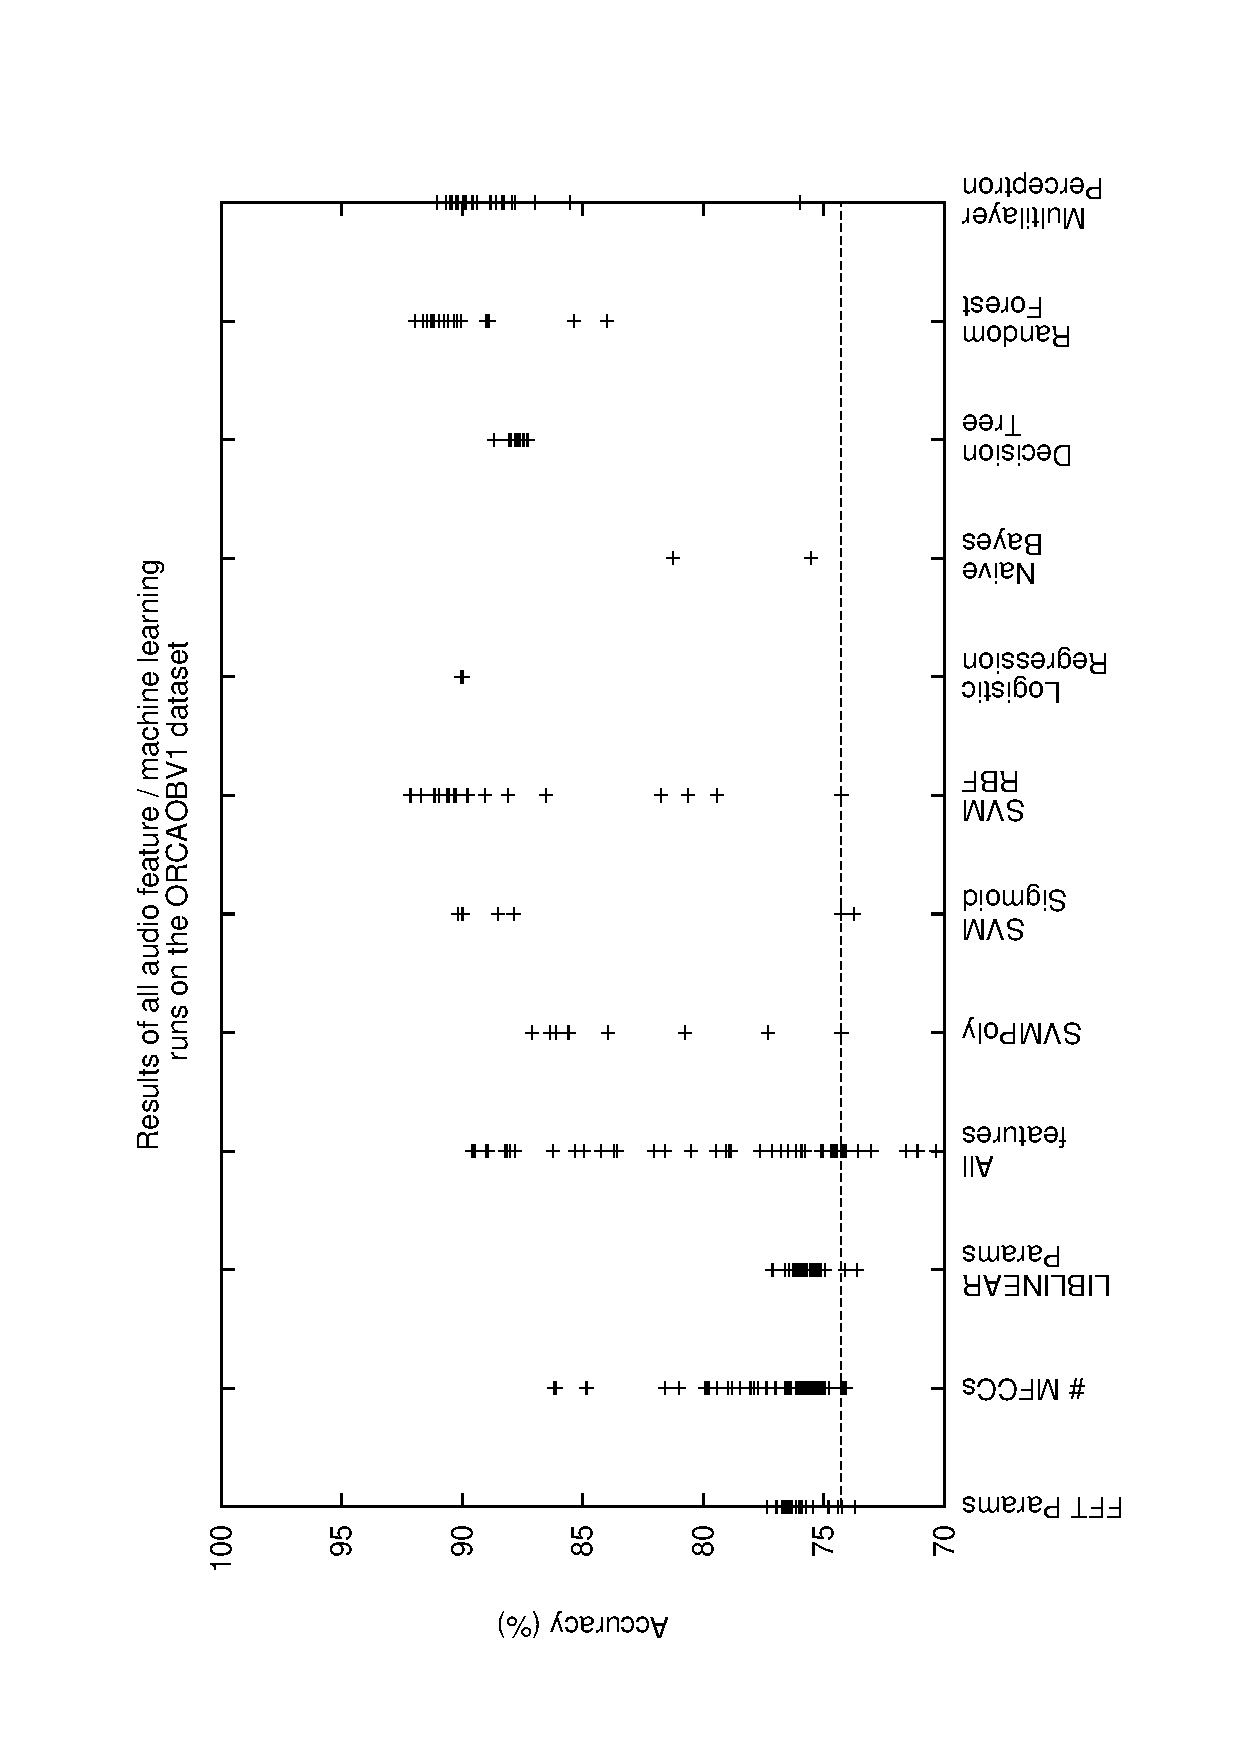
\includegraphics[width=\columnwidth]{figures/gnuplot-obv-all-data}
\caption{Shown are 831 data points from all the runs with different
  combinations of audio features and classifier and different
  parameter settings for each.}
\label{fig:gnuplot-obv-all-data}
\end{figure}

From these tables we can see that choosing an appropriate set of audio
feature extractors and machine learning algorithm can lead to good
classification performance.  When the various hyper-parameters of
these algorithms are optimized, even better performance can be
obtained.  When using only 13 MFCCs and an SVM with a linear kernel,
the maximum classification accuracy that was obtained was a poor
76.97\%, as can be seen in Table \ref{table:obv-fft}.  Increasing the
number of MFCC coefficients surprisingly greatly increased the
performance of the orca/background/voice classification task, and as
shown in Table \ref{table:obv-numMfccs} the highest classification
accuracy obtained was 86.17\%.  This is not usually a parameter that
needs to be adjusted when studying human speech or music, therefore this is a
surprising result.  As more features were added classification
performance increased in general.  This is a different result than was
obtained using a smaller dataset where the addition of Yin features
hurt performance \cite{ness2008chants}.  The maximum classification
accuracy was obtained using 70 MFCC coefficents and all possible audio
features.  For future work, it would be interesting to look at
including even more audio features, to see if the classification
accuracy continues to increase.

After finding the optimal audio features using an SVM with a linear
kernel, these features were used as input to a series of machine
learning classifiers.  The lowest performers were SVM with a
polynomial kernel (76.92\%), Naive Bayes (81.25\%).  The rest of the
learners performed well, with Decision Trees giving a maximum accuracy
of 88.67\%, Linear SVM of 89.53\%, Logistic Regression at 90.04\%, SVM
with a Sigmoid kernel of 90.18\%, Multilayer Perceptron at 91.04\%,
Random Forest with 91.97\%, and SVM with a Radial Basis Function
kernel at 92.12\%.  ALl the accuracy results in this chapter are
show in Figure \ref{fig:gnuplot-obv-all-data}.  In this figure, a
dashed line at 74.26\% represents the performance of the ZeroR
classifier.  From this graph we can see the SVM with an RBF kernel
performed the best, but that the Random Forest classifier was close
behind.  All the audio feature / classifier combinations showed
dramatic performance changes when parameters were changed, which
highlights the importance of doing parameter searches.

However, when doing actual classification experiments, it must be
decided if the rise in classification performance is offset by the
training and testing time.  For the LIBLINEAR classifier to obtain a
performance of 89.53\%, it took 18.3 minutes to train and predict the
ORCAOBV1 dataset.  For SVM with an RBF kernel it took 19.4 hours to do
the same thing, which means that it took almost a two-fold increase in
order of magnitude in time for a 2.59\% rise in performance.


\section{Scaling and Grid Computation}


The purpose of these experiments is to find the combination of audio
features and machine learning algorithm that gives the highest
performance for segmenting recordings into orca/background/voice, and
to then use this combination to predict classes for all recordings in
the Orchive.  In order to investigate the performance of the
classification of recordings into orca, background and voice, we
trained a SVM with a section of 30 and 240 seconds of hand trimmed
data.

These results were generated using the bextract/sfplugin combination
from \textit{Marsyas}, which are two different programs, the first of which
``bextract'' extracts audio features from a collection of audio files
and trains a machine learning classifier.  This trained classifier is
then used by the ``sfplugin'' program to extract audio features from
an audio source and to classify it.  The sfplugin program allows for
feature extraction and machine learning in a single executable, which
allows for a dramatic speedup because audio features do not need to be
written to disk and reread from disk.  In this hybrid program, audio
features train the machine learning system directly.

I first trained a model with bextract, and then used the sfplugin
program in \textit{Marsyas} to classify all the recordings in the Orchive on
the Hermes/Nestor cluster, part of the Westgrid computational
resource.  For this, I divided the data into sets of 1\%, 5\%, 10\%
and 100\% of the Orchive.  The timing results of these datasets run on
10 computers are shown in Table \ref{table:full-orchive-performance}.
From this, we can see that the classifier that had more data took
longer to classify, and that the speedup from taking samples of the
data was almost linear.


\begin{table}
\centering
\begin{tabular}{|c|c|c|} 
\hline
Training data & \% of Orchive & Run time \\
\hhline{|~|~|~|}
 (sec)        &               & (DD:HH:MM:SS) \\
\hhline{|=|=|=|}
30            &      1      &    00:00:05:18      	 \\
30            &      5      &    00:00:25:20         \\
30            &      10     &    00:00:50:58         \\
30            &      100    &    00:09:01:05         \\
\hline
240           &      1      &    00:06:16            \\
240           &      5      &    00:00:31:21         \\
240           &      10     &    00:04:47:12         \\
240           &      100    &    02:04:18:32         \\
\hline
\end{tabular}
\caption{Performance results of timing on subsets of the entire
  Orchive dataset using ten 2.66-GHz Intel Xeon x5650 cores.}
\label{table:full-orchive-performance}
\end{table}

%
% Downsampling
%
\section{Downsampling}

One way to reduce the total number of feature vectors, thereby
lowering feature size on disk and decreasing the training time and
testing time for machine learning classifiers is to downsample the
feature vectors at the time that features are calculated.  In this
case, downsampling is done by only outputting one feature vector each
$N$ times the feature is calculated.  In Table
\ref{table:obv-downsampling}, results are shown for using window sizes
from 512 to 4096 and downsampling rates from 1, where every feature
vector is output to 1000, where only every 1000th feature vector is
used.  What one would expect in this table is that a downsampling of 1
would give the highest accuracy, and greater amounts of downsampling
should either give the same accuracy until too few feature vectors are
used and performance would decrease.  In this table, the accuracy is
quite similar inside a single window size, for example, for the case
of a window size of 512, the difference in accuracies is 1.21\%.  This
tells us that in general, with the large amount of data that is in
this training set, any amount of downsampling will give approximately
the same results.  This could be used to great effectiveness when
expanding the set of the training data to a larger size than the
11,041 clips used in this section as is shown by the dramatic
reduction in training and test times that are seen in Table
\ref{table:obv-downsampling}.

\begin{table}
\begin{tabular}{|l|l|l|l|l|l|}
\hline
\multicolumn{3}{|c|}{FFT param} & \multicolumn{2}{c|}{Time (sec)} & Accuracy \\
\hhline{|-|-|-|-|-|~|}
ws & hp & downsampling & Train & Predict & \multicolumn{1}{c|}{(\%)} \\
\hhline{|=|=|=|=|=|=|}
512 & 256 & 1       &    31.27  &  2.06  &  75.90  \\
512 & 256 & 10      &     3.26  &  0.21  &  76.01  \\
512 & 256 & 100     &     0.31  &  0.03  &  75.82  \\
512 & 256 & 1000    &     0.07  &  0.02  &  75.00  \\
1024 & 512 & 1      &    17.80  &  1.05  &  75.76  \\
1024 & 512 & 10     &     1.64  &  0.12  &  75.76  \\
1024 & 512 & 100    &     0.15  &  0.02  &  76.52  \\
1024 & 512 & 1000   &     0.02  &  0.00  &  77.67  \\
\hline
2048 & 1024 & 1     &     8.60  &  0.52  &  75.92  \\
2048 & 1024 & 10    &     0.86  &  0.06  &  75.96  \\
2048 & 1024 & 100   &     0.08  &  0.01  &  74.90  \\
2048 & 1024 & 1000  &     0.01  &  0.00  &  73.08  \\
4096 & 2048 & 1     &     3.96  &  0.30  &  75.93  \\
4096 & 2048 & 10    &     0.36  &  0.04  &  75.89  \\
4096 & 2048 & 100   &     0.09  &  0.01  &  \textbf{76.54}  \\
4096 & 2048 & 1000  &     0.03  &  0.02  &  57.69  \\
\hline
\end{tabular}
\caption{Table showing the results of different amounts of
  downsampling on classification performance with the LIBLINEAR SVM
  using MFCC audio features.  Note that approximately 3x as
  much data points as this were calculated but were omitted due to
  space.  These omitted data points showed the same approximate
  performance as those shown here.}
\label{table:obv-downsampling}
\end{table}

For each of these machine learning methods, a confusion matrix was
obtained. This matrix shows the distribution of predictions and
mispredictions for each class. If the dataset had been perfectly
classified all the classifications would fall on the diagonal.  The
confusion matrix for one of the settings of the Random Forest is shown
in Table \ref{table:OBVConfusionMatrix}.  From this table, one can see
that in the majority of cases, the classifier predicted the label
correctly, but that in the case of background labels, there were a
large number of background labels that were predicted as orca calls at
a level of approximately 26\%.  The inverse of this, where orca calls
were misclassified as background was much lower, with a
misclassification rate of approximately 4\%.  For this task, the time
taken to build model was 1279 seconds and the time taken to test the
model on training data was 34 seconds on a 2.67-GHz Xeon x5550
processor.

\begin{table}
\begin{tabular}{|c|c|c|c|}
\hline
           & background & orca & voice \\
\hline
background & 79.4 &  20.5  &  0.1      \\
orca       & 3.7  &  96.1  &  0.1      \\
voice      & 1.0  &  13.3  &  85.7     \\
\hline
\end{tabular}
\caption{Confusion matrix for the Random Forest machine
  learning classifier.  The labels along the top represent the
  classifications by the machine learning classifier and those on the
  left side show the ground truth.  For a classifier that predicts
  each label perfectly, all the numbers would be on the diagonal. From
  this we can see that the majority of labels predicted classifier
  match the ground truth, but that the classifier mispredicts
  background labels as orca calls at a level of approximately 26\%.  }
\label{table:OBVConfusionMatrix}
\end{table}

However, in some cases, higher accuracies for larger downsampling
rates is seen.  Upon further investigation, this turned out to be due
to the fact that many clips were of short duration, with many being
approximately 0.2 seconds in length.  At this resolution, all of the
feature vectors for some of these short recordings were discarded, and
they did not become part of either the training or test set.  For this
reason, all subsequent tables do not use downsampling, and to
accommodate the long training and prediction times, a large cluster
was used, and each job was given the maximum allowable three-day run
time to complete.


\section{Call classification}

Once the large amount of data has been segmented into sections that
have been identified as orca calls, I am now interested in
classifying these call types based on the call catalog of Ford
\cite{ford1987catalogue}.  As an additional and related task, I am
also interested in classifying these call types based on the clan, pod,
subpod, matriline and individual that made the calls.  These are
overlapping tasks as some call types are only made by one pod, so
classifying some of them would automatically give the pod they came
from, like the N47 call.  Other call types are very distinct from pod to
pod, and can be handled as separate classification tasks, and others
are so similar, like N3, that it is difficult for an untrained person
to differentiate between call types made by different pods and would likely
be a difficult machine learning task.

I name the call catalog dataset used in this section ORCACALL1.  It
contains 2954 different clips containing orca calls as labelled by
people trained to do NRKW orca call classification.  The names,
numbers of instances in the ORCACALL1 dataset, and a few spectrograms
of representative exemplars are shown in Table
\ref{table:calls-table}.  It should be noted that the call types are
not present in equal abundance as a number of the call types are less
frequently vocalized by the orcas in the recordings that were
examined.  Some of the less frequently found call types are N08, N10,
N23 and N25.  Because of this inequal class distribution, a ZeroR
classifier would give a classification accuracy of 45\%; If the
classes had equal numbers of instances, the performance of the ZeroR
classifier would be 8.3\%.  For the work in this thesis, it was
determined that having a wider set of instances for training would be
preferable to the dramatic pruning that would have to occur if the
largest class (N04 : 1281 instances) would have to be pruned to the
size of the smallest (N08 : 22 instances).  Work is ongoing in the
creation of the ORCACALL2 dataset, which will have a wider set of call
types and more instances of all call types, with preference given to
less frequently produced call types.

The clips for this were obtained directly from the expert users, and
often contained small amounts of silence or boat noise before and
after the clip.  In addition, many of the clips contained very distant
orca calls, so distant that the calls were not clearly visible on the
spectrogram through the noise.  I concatentated all the clips
together, and generated a dataset where only the calls that were
visible in the spectrogram are represented, this gave a dataset of
1566 clips.  However, many of these clips were still quiet distant, so
I generated a second dataset of just the loud calls, which gave a
dataset of 658 calls.  These clips were run through the same
processing steps below as the untrimmed clips, and results are
presented alongside them.

\begin{table}
\begin{tabular}{|l|l|l|l|l|}
\hline
Call     &  \# Calls  & \# Trimmed & \# Trimmed         &  Representative  \\
type     &            & calls      & loud calls         &    spectrogram    \\
\hline
 N01     &  364       &  296  &   85                &   \includegraphics[height=1.5cm] {figures/catalog/A36-N01-062802-D004-12218.png} \\ \hline
 N02     &  123       &   95  &   53                &   \includegraphics[height=1.5cm] {figures/catalog/A36-N02-063002-D005-10750.png} \\ \hline
 N03     &  244       &  106  &   56                &   \includegraphics[height=1.5cm] {figures/catalog/A36-N03-071506-D017-10139.png} \\ \hline
 N04     &  1281      &  281  &   64                &   \includegraphics[height=1.5cm]  {figures/catalog/A36-N04-063002-D005-10843.png} \\ \hline
 N05     &  157       &  142  &   74                &   \includegraphics[height=1.5cm] {figures/catalog/A35-N05-070606-D011-04146.png} \\ \hline
\end{tabular}
\caption{Part 1 of table of call types in the ORCACALL1 dataset.  All call types were
  annotated by users trained in recognizing orca vocalizations.  Some
  call types, such as N04 are more frequently vocalized by orcas, and are
  present in higher abundance in this dataset.  Work is ongoing in
  creating the ORCACALL2 dataset, which will have a larger set of
  call types.}
\label{table:calls-table}
\end{table}

\begin{table}
\begin{tabular}{|l|l|l|l|l|}
\hline
Call     &  \# Calls  & \# Trimmed & \# Trimmed         &  Representative  \\
type     &            & calls      & loud calls         &  spectrogram    \\
\hline
 N07     &   108      &             91  &   59                    &  \includegraphics[height=1.5cm] {figures/catalog/A08-N07-071110-D013-01151.png} \\ \hline
 N08     &   22       &             10  &    5                    &  \includegraphics[height=1.5cm] {figures/catalog/A04-N08-071906-D020-13145.png} \\ \hline
 N09     &   413      &            328  &  129                    &  \includegraphics[height=1.5cm] {figures/catalog/A12-N09-070102-D005-14103.png} \\ \hline
 N10     &   39       &             26  &   19                    &  \includegraphics[height=1.5cm] {figures/catalog/A36-N10-063002-D005-10954.png} \\ \hline
 N23     &   30       &             18  &    9                    &  \includegraphics[height=1.5cm] {figures/catalog/I31-N23-070706-D011-10950.png} \\ \hline
 N25     &   27       &             12  &    6                    &  \includegraphics[height=1.5cm] {figures/catalog/I15-N25-081206-D044-02059.png} \\ \hline
 N47     &   177      &            161  &   99                    &  \includegraphics[height=1.5cm] {figures/catalog/A12-N47-080210-D056-15012.png} \\ \hline
\end{tabular}
\caption{Part 2 of table of call types in the ORCACALL1 dataset.}
\label{table:calls-table}
\end{table}

It should be noted though that there are other forms of information
that can be used by scientists in the future when using classifiers
from this work, the most important being direct visual observation
combined with the use of the photo identification catalog.  This could
be combined with acoustic arrays of hydrophones to localize individual
whales.

In this section, I will follow a similar strategy to that for the
classification task above and will discuss the similarities and
differences when classifying call types as opposed to simply classifying
audio into orca/background/voice as in the ORCAOBV1 dataset.  The
dataset with call types will be referred to as ORCACALL1 in the following
tables.

In order to classify the clips in the ORCACALL1 dataset, I use a
different experimental procedure to that used in the ORCAOBV1 results
presented in the previous section.  Each clip was considered to have
been presegmented by either the user or the machine learning system
and results on a per clip-level were generated.  These clip level
decisions were made using a voting metaphor, where each feature vector
in a clip was assigned a label by the classifier individually, and the
clip was labeled with the label that occurred the most often.

%
% FFT Parameters
%
\subsection{FFT Parameters}

Following a similar procedure to that carried out for ORCAOBV1
dataset, a parameter scan of different window sizes, hop sizes and
texture window sizes was performed, with results shown in Table
\ref{table:calls-fft}.  In this table, there is a larger variation in
accuracy than was seen in the case of the ORCAOBV1 dataset and the
highest accuracy that was obtained was 56\%, which was obtained with a
window size of 4096 and a memory size of 10 for the trimmed loud
clips.  However, the results for a window size of 2048 and a memory
size of 10 gave almost the same results of 55\% but with half as long
an integration time, thus allowing for shorter integration
times. Because of this, for subsequent tables, a window size of 2048,
hop size of 1024 and memory size of 10 was used to facilitate
comparison with the results for the ORCAOBV1 dataset.  It is
interesting to note that the trimmed clips did approximately as well
as the untrimmed clips, however the trimmed loud clips had higher
accuracy.  This can be explained by the fact that MFCC features are
cepstrums, which are spectrums of spectrums, and for clips with a
larger signal in them, the feature vectors obtained would be more
distinct from noise vectors for loud clips than for quiet clips.

\begin{table}
\begin{tabular}{|c|c|c|c|c|c|c|c|}
\hline
\multicolumn{3}{|c|}{FFT param} & \multicolumn{2}{c|}{Time (sec)} & \multicolumn{3}{c|}{\% Accuracy} \\
\hhline{|-|-|-|-|-|-|-|-|}
ws & hp & mem & Extract & Train & All & Trimmed & Trimmed Loud \\
\hhline{|=|=|=|=|=|=|=|=|}
512  & 256  & 1    &    141.79  &    87.32  &  47  & 39 & 48 \\
512  & 256  & 2    &    127.92  &   505.95  &  47  & 44 & 50 \\
512  & 256  & 5    &    153.62  &   314.00  &  48  & 46 & 50 \\
512  & 256  & 10   &    140.79  &   339.46  &  48  & 45 & 50 \\
512  & 256  & 20   &    118.44  &   368.40  &  49  & 48 & 50 \\
\hline
1024 & 512  & 1    &     90.56  &    30.82  &  44  & 39 & 44 \\
1024 & 512  & 2    &    117.79  &   177.41  &  48  & 44 & 47 \\
1024 & 512  & 5    &    108.07  &   178.74  &  48  & 45 & 52 \\
1024 & 512  & 10   &    102.28  &   137.23  &  50  & 48 & 53 \\
1024 & 512  & 20   &     92.13  &   151.60  &  51  & 49 & 55 \\
\hline
2048 & 1024 & 1    &     86.24  &    13.75  &  44  & 43 & 47 \\
2048 & 1024 & 2    &     83.15  &   118.59  &  49  & 48 & 47 \\
2048 & 1024 & 5    &     72.37  &    69.04  &  49  & 51 & 52 \\
2048 & 1024 & 10   &     85.48  &    62.31  &  52  & 48 & 55 \\
2048 & 1024 & 20   &     78.48  &    85.45  &  52  & 48 & 55 \\
\hline
4096 & 2048 & 1    &     76.07  &     5.34  &  46  & 46 & 47 \\
4096 & 2048 & 2    &     83.15  &    38.11  &  49  & 47 & 48 \\
4096 & 2048 & 5    &     72.37  &    30.38  &  51  & 50 & \textbf{56} \\
4096 & 2048 & 10   &     75.06  &    28.24  &  52  & 47 & 53\\
4096 & 2048 & 20   &     77.32  &    27.35  &  52  & 48 & 55 \\
\hline
\end{tabular}
\caption{Table of MFCC results with different window
  sizes using the LIBLINEAR classifier.  In this and subsequent
  tables, ``ws'' refers to the size of the FFT window in samples,
  ``hp'' refers the hop size between sequent FFT frames in samples,
  and ``mem'' refers to the size of the texture window in frames.
  Longer texture window sizes have been omitted as they showed
  anomalous behaviour due to the short size of the clips as compared
  to the long integration time.}
\label{table:calls-fft}
\end{table}

%
% Different numbers of MFCCs
%
\subsection{Number of MFCC coefficients}

As in the ORCAOBV1 dataset, a parameter scan of the number of MFCC
components was carried out, with results shown in Table
\ref{table:calls-numMfccs}.  The highest performance obtained was for
a window size of 4096 and 100 MFCCs with an accuracy of 58\%, with a
window size of 2048 and 100 MFCCs yielding an accuracy of 54\%.  These
results show a similar trend to the results obtained for ORCAOBV1 with
more MFCCs giving better results.  Using a window size of 4096 samples
with a hop size of 2048 samples at 44100 samples/sec gives an
integration time of 46.4 milliseconds, and 10 of these windows (given
a memory size of 10 frames) would result in a total time of 464
milliseconds or almost half a second.  Using a window size of 2048
would give a total time of half that or 232 milliseconds.  Like in
Table \ref{table:calls-fft} the performance of classifiers with loud
trimmed clips did significantly better than for untrimmed and the
whole set of trimmed clips.  This is likely due to the fact that for
clips with greater signal, MFCC features produce feature vectors that
are more distinct from clips with less signal, or clips of boat noise.

\begin{table}
%% \begin{tabular}{|l|l|l|l|l|l|}
%% \hline
%% \multicolumn{3}{|c}{FFT param} & \multicolumn{1}{|c|}{Time (sec)} & Accuracy \\
%% \hhline{|-|-|-|-|~|}
%% ws & hp & Num MFCCs & Train & \multicolumn{1}{c|}{(\%)} \\
%% \hhline{|=|=|=|=|=|}
\begin{tabular}{|c|c|c|c|c|c|c|c}
\hline
\multicolumn{3}{|c|}{FFT param} & \multicolumn{1}{c|}{Time (sec)} & \multicolumn{3}{c|}{\% Accuracy} \\
\hhline{|-|-|-|-|-|-|-|-|}
ws & hp & mem & Train & All & Trimmed & Trimmed Loud \\
\hhline{|=|=|=|=|=|=|=|=|}
512 & 256 & 1      &        30.86  &    43   &  21  &  21 \\
512 & 256 & 5      &       125.01  &    43   &  36  &  41 \\
512 & 256 & 10     &       217.63  &    48   &  46  &  50 \\
512 & 256 & 15     &       325.26  &    49   &  47  &  53 \\
512 & 256 & 25     &       675.81  &    51   &  54  &  58 \\
512 & 256 & 30     &      1059.44  &    51   &  53  &  59 \\
512 & 256 & 40     &      1153.37  &    51   &  54  &  61 \\
\hline
1024 & 512 & 1     &        15.20  &    43  &  21  &  21 \\
1024 & 512 & 5     &        50.34  &    43  &  36  &  41 \\
1024 & 512 & 10    &       122.80  &    49  &  46  &  50 \\
1024 & 512 & 15    &       155.82  &    50  &  49  &  55 \\
1024 & 512 & 25    &       336.11  &    52  &  55  &  56 \\
1024 & 512 & 50    &       836.08  &    53  &  58  &  58 \\
1024 & 512 & 70    &      1850.25  &    53  &  57  &  56 \\
1024 & 512 & 100   &      2667.66  &    53  &  60  &  62 \\
\hline
2048 & 1024 & 1    &         5.24  &    43 &  21  &  21 \\
2048 & 1024 & 5    &        22.52  &    44 &  35  &  38 \\
2048 & 1024 & 10   &        50.33  &    49 &  46  &  52 \\
2048 & 1024 & 15   &        75.94  &    51 &  51  &  56 \\
2048 & 1024 & 25   &       192.55  &    53 &  58  &  56 \\
2048 & 1024 & 50   &       524.04  &    54 &  60  &  62 \\
2048 & 1024 & 70   &       887.34  &    54 &  60  &  62 \\
2048 & 1024 & 100  &      1474.60  &    54 &  59  &  62 \\
\hline
4096 & 2048 & 1    &         2.51  &    43 &  20  &  21 \\
4096 & 2048 & 5    &         9.18  &    44 &  31  &  38 \\
4096 & 2048 & 10   &        21.19  &    50 &  41  &  50 \\
4096 & 2048 & 15   &        34.65  &    54 &  48  &  50 \\
4096 & 2048 & 25   &        78.55  &    57 &  57  &  56 \\
4096 & 2048 & 50   &       213.46  &    58 &  57  &  \textbf{67} \\
4096 & 2048 & 70   &       346.59  &    58 &  57  &  \textbf{67} \\
4096 & 2048 & 100  &       668.68  &    58 &  56  &  65 \\
\hline
\end{tabular}
\caption{Table of MFCC results with different numbers of MFCC
  coefficients using the LIBLINEAR classifier and the ORCACALL1 dataset}
\label{table:calls-numMfccs}
\end{table}

%
% LIBLINEAR parameters
%
\subsection{LIBLINEAR parameters}

A parameter sweep of using different solvers and values of C for
LIBLINEAR was then carried out, with results shown in Table
\ref{table:calls-liblinear}.  In this table, several experimental
conditions gave the same performance of 55\%.  However, unlike in the
ORCAOBV1 case, there was considerably more variation in performance
with this classifier.  In terms of speed, the L2-regularized L2-loss
support vector classification (primal) gave the fastest consistent
performance as can be seen in Figure
\ref{fig:gnuplot-calls-liblinear-time}.  What is interesting here is
that even though the different values of C do not cause big
differences in classification accuracy, depending on the solver, they
can a have dramatic impact on the time it takes to reach a solution.
For this dataset, it appears that the best solver with the most
consistent performance is the L2-regularized L2-loss support vector
classification (primal).  In these experiments, again the set of
trimmed loud clips performed better, which is expected for clips with
a greater signal in them with MFCC features.

\begin{figure}[t]
\centering
\includegraphics[width=\columnwidth]{figures/gnuplot-calls-liblinear-time}
\caption{The amount of time that different solvers took to train a SVM
  model in LIBLINEAR.}
\label{fig:gnuplot-calls-liblinear-time}
\end{figure}


\begin{table}
%% \begin{tabular}{|l|l|l|l|}
%% \hline
%% \multicolumn{2}{|c}{LIBLINEAR param} & \multicolumn{1}{|c|}{Time (sec)} &  Accuracy \\
%% \hhline{|-|-|-|~|}
%% Solver & C & Train & \multicolumn{1}{c|}{(\%)} \\
%% \hhline{|=|=|=|=|}
\begin{tabular}{|c|c|c|c|c|c|}
\hline
\multicolumn{2}{|c|}{LIBLINEAR param} & \multicolumn{1}{c|}{Time (sec)} & \multicolumn{3}{c|}{\% Accuracy} \\
\hhline{|-|-|-|-|-|-|}
Solver & C & Train & All & Trimmed & Trimmed Loud \\
\hhline{|=|=|=|=|=|=|}
1 & 0.001   &       3.71  &    51  &  43  &  50 \\
1 & 1.0     &      31.16  &    53  &  45  &  50 \\
1 & 100.0   &     405.72  &    43  &  42  &  33 \\
2 & 0.001   &       3.55  &    51  &  44  &  50 \\
2 & 1.0     &       3.73  &    53  &  45  &  50 \\
2 & 1000.0  &       3.78  &    53  &  45  &  50 \\
\hline
3 & 0.001   &       3.40  &    51  &  50  &  \textbf{55} \\
3 & 1.0     &      18.84  &    54  &  52  &  53 \\
3 & 1000.0  &     425.39  &    33  &  35  &  50 \\
4 & 0.001   &       2.28  &    49  &  47  &  \textbf{55} \\
4 & 1.0     &      32.90  &    52  &  49  &  \textbf{55} \\
4 & 1000.0  &    9557.33  &    46  &  48  &  \textbf{55} \\
\hline
5 & 0.001   &      15.43  &    47   &  43  &  53 \\
5 & 1.0     &      34.04  &    53   &  45  &  50 \\
5 & 1000.0  &      31.91  &    53   &  45  &  50 \\
6 & 0.001   &       5.52  &    43   &  39  &  41 \\
6 & 1.0     &      14.32  &    54   &  46  &  52 \\
6 & 1000.0  &      17.12  &    54   &  45  &  53 \\
7 & 0.001   &       5.20  &    45   &  41  &  41 \\
7 & 1.0     &      12.45  &    54   &  48  &  53 \\
7 & 1000.0  &     635.40  &    50   &  48  &  53 \\
\hline
\end{tabular}
\caption{A table showing the results with the ORCACALL1 dataset of
  doing a parameter search over a wide number of values of C and using
  the different solvers in the LIBLINEAR package.}
\label{table:calls-liblinear}
\end{table}

%
% MIR Features
%
\subsection{MIR Features}

In order to investigate the manner in which different audio features
affect classification performance, a series of experiments was carried
out in which different audio features and combinations of these audio
features was used, with a similar methodology to that used on the
ORCAOBV1 dataset.

%% In the first test, different window and hop sizes were used as input
%% to the MFCC algorithm, with a texture memory size set at 10.  These
%% results are shown in Table \ref{table:calls-different-mfcc}.  Unlike
%% in the ORCAOBV1 case, the best classification accuracy was obtained
%% for longer window sizes, with the best performance being at a window
%% size of 4096, which gave a classification accuracy of 53\%.

%% \begin{table}
%% %% \begin{tabular}{|l|l|l|l|l|}
%% %% \hline
%% %% \multicolumn{2}{|c|}{FFT param} & \multicolumn{2}{c|}{Time (sec)} & Accuracy \\
%% %% \hhline{|-|-|-|-|~|}
%% %% ws & hp & Extract & Train &  \multicolumn{1}{c|}{(\%)} \\
%% %% \hhline{|=|=|=|=|=|}
%% \begin{tabular}{|c|c|c|c|c|c|c|c|}
%% \hline
%% \multicolumn{3}{|c|}{FFT param} & \multicolumn{2}{c|}{Time (sec)} & \multicolumn{3}{c|}{\% Accuracy} \\
%% \hhline{|-|-|-|-|-|-|-|-|}
%% ws & hp &  Extract & Train & All & Trimmed & Trimmed Loud \\
%% \hhline{|=|=|=|=|=|=|=|=|}
%% 256 & 128 &    228.01  &   70.64  &    47  \\
%% 512 & 256 &    176.47  &   28.56  &    48  \\
%% 1024 & 512 &   131.70  &   15.56  &    49  \\
%% 2048 & 1024 &  102.47  &    7.60  &    51  \\
%% 4096 & 2048 &   98.47  &    3.62  &    53  \\
%% \hline
%% \end{tabular}
%% \caption{Table showing the classification accuracy and timing when
%%   using different FFT window sizes on MFCC features using a linear SVM
%%   kernel using the ORCACALL1 dataset.}
%% \label{table:calls-different-mfcc}
%% \end{table}

When the RMS feature alone was used, a dramatic drop in performance
was seen, with the accuracy in each window size being 43\% as is seen
in Table \ref{table:calls-different-rms}.  This is an expected
behaviour because with the ORCACALL1 database the loudness of
different call types is uncorrelated with the call type and is
dependent instead on the distance of the orca from the hydrophone.  It
is also interesting that for the trimmed calls and trimmed loud calls
that the accuracy was very low, this is likely because the untrimmed
clips were actually being classified due to the amount of noise in
them, not in their actual performance on classifying different calls.
It is very interesting that for RMS features, the trimmed and trimmed
loud clips performed much more poorly than the untrimmed calls.  This
is likely due to the classification algorithm actually classifying the
untrimmed clips based on the amount of noise in them, rather than on
the actual signal in them.  Given the nature of the RMS feature, that
it basically is a measure of the loudness of a clip, this is a likely
outcome, and shows us that on their own, RMS features are not a good
way to classify calls.

\begin{table}
%% \begin{tabular}{|l|l|l|l|l|}
%% \hline
%% \multicolumn{2}{|c|}{FFT param} & \multicolumn{2}{c|}{Time (sec)} & Accuracy \\
%% \hhline{|-|-|-|-|~|}
%% ws & hp & Extract & Train &  \multicolumn{1}{c|}{(\%)} \\
%% \hhline{|=|=|=|=|=|}
\begin{tabular}{|c|c|c|c|c|c|c|}
\hline
\multicolumn{2}{|c|}{FFT param} & \multicolumn{2}{c|}{Time (sec)} & \multicolumn{3}{c|}{\% Accuracy} \\
\hhline{|-|-|-|-|-|-|-|}
ws & hp & Extract & Train & All & Trimmed & Trimmed Loud \\
\hhline{|=|=|=|=|=|=|=|}
256 & 128        &   178.01  &    7.00  &    \textbf{43}  & 17 & 20 \\
512 & 256        &   135.04  &    3.41  &    \textbf{43}  & 23 & 20 \\
1024 & 512       &   100.13  &    1.66  &    \textbf{43}  & 22 & 20 \\
2048 & 1024      &    88.20  &    0.82  &    \textbf{43}  & 22 & 20  \\
4096 & 2048      &    86.54  &    0.33  &    \textbf{43}  & 22 & 20 \\
\hline
\end{tabular}
\caption{Table using audio from the ORCACALL1 dataset showing the
  effect of window size on classification performance with LIBLINEAR
  using the Root Mean Square (RMS) energy of a signal as a feature.}
\label{table:calls-different-rms}
\end{table}

Surprisingly, the use of statistical measures of the spectrum, as
shown in Table \ref{table:calls-different-spectral}, gave poor
classification accuracy, with a maximum classification accuracy of
43\%.  This is likely because the broad spectral characteristics of
these measures did not accurately capture important factors about the
differences between calls.  Another confounding factor is the
directionality of calls which means that the orientation of the
vocalizing orca to the receiving hydrophone is a confounding variable
here \cite{miller2002mixed}.  The results for trimmed and untrimmed
calls are also low, as was seen for RMS, which is likely because in
the case of untrimmed clips, the classifier was actually classifying
the clips by the spectral characteristics of the noise in the
untrimmed clips, and not classifying the actual calls.  Like in the
case of RMS features, the trimmed and untrimmed clips perform
significantly worse than untrimmed clips, but in this case instead of
the loudness of a clip, the classifier was likely taking advantage of
the spectral characteristics of noise in the untrimmed clips.

\begin{table}
%% \begin{tabular}{|l|l|l|l|l|l|}
%% \hline
%% \multicolumn{1}{|c|}{Feature} &\multicolumn{2}{c|}{FFT param} & \multicolumn{2}{c|}{Time (sec)} & Accuracy \\
%% \hhline{|~|-|-|-|-|~|}
%% Extractor & ws & hp & Extract & Train  &  \multicolumn{1}{c|}{(\%)} \\
%% \hhline{|=|=|=|=|=|=|}
\begin{tabular}{|c|c|c|c|c|c|c|c|}
\hline
\multicolumn{3}{|c|}{FFT param} & \multicolumn{2}{c|}{Time (sec)} & \multicolumn{3}{c|}{\% Accuracy} \\
\hhline{|-|-|-|-|-|-|-|-|}
ws & hp & mem & Extract & Train & All & Trimmed & Trimmed Loud \\
\hhline{|=|=|=|=|=|=|=|=|}
centroid & 256 & 128       &   215.26  &    6.99  &  \textbf{43}  & 26 & 20 \\
centroid & 512 & 256       &   144.23  &    3.10  &  \textbf{43}  & 26 & 20 \\
centroid & 1024 & 512      &   119.32  &    1.58  &  \textbf{43}  & 25 & 20 \\
centroid & 2048 & 1024     &   102.19  &    0.85  &  \textbf{43}  & 25 & 20 \\
centroid & 4096 & 2048     &    96.78  &    0.32  &  \textbf{43}  & 22 & 18 \\
\hline
flux & 256 & 128           &   218.31  &    7.43  &  \textbf{43}  & 21 & 20 \\
flux & 512 & 256           &   145.60  &    3.49  &  \textbf{43}  & 12 & 20 \\
flux & 1024 & 512          &   130.55  &    1.69  &  \textbf{43}  & 21 & 20 \\
flux & 2048 & 1024         &   107.72  &    0.91  &  \textbf{43}  & 21 & 20 \\
flux & 4096 & 2048         &    95.93  &    0.39  &  \textbf{43}  & 21 & 20 \\
\hline
rolloff & 256 & 128        &   205.94  &    6.08  &  \textbf{43}  & 31 & 17 \\
rolloff & 512 & 256        &   151.70  &    6.37  &  \textbf{43}  & 25 & 17 \\
rolloff & 1024 & 512       &   117.73  &    1.42  &  \textbf{43}  & 31 & 20 \\
rolloff & 2048 & 1024      &   109.10  &    0.71  &  \textbf{43}  & 31 & 20 \\
rolloff & 4096 & 2048      &    96.30  &    0.30  &  \textbf{43}  & 32 & 18 \\
\hline
kurtosis & 256 & 128       &   212.50  &    7.14  &  42           & 22 & 23 \\
kurtosis & 512 & 256       &   145.55  &    3.30  &  42           & 20 & 20 \\
kurtosis & 1024 & 512      &   123.56  &    1.91  &  \textbf{43}  & 22 & 23 \\
kurtosis & 2048 & 1024     &   108.91  &    0.74  &  42           & 23 & 21 \\
kurtosis & 4096 & 2048     &    95.63  &    0.39  &  42           & 23 & 21 \\
\hline
skewness & 256 & 128       &   232.54  &    7.31  &  \textbf{43}  & 23 & 20  \\
skewness & 512 & 256       &   179.31  &    3.51  &  \textbf{43}  & 25 & 23 \\
skewness & 1024 & 512      &   202.36  &    1.79  &  \textbf{43}  & 18 & 20 \\
skewness & 2048 & 1024     &   317.77  &    0.66  &  42           & 24 & 20 \\
skewness & 4096 & 2048     &   571.55  &    0.38  &  \textbf{43}  & 25 & 21 \\
\hline
\end{tabular}
\caption{Table showing the effect of using
  combinations of different statistical measures of the spectrum of a
  signal on classification performance with LIBLINEAR.}
\label{table:calls-different-spectral}
\end{table}

However, when using a combination of Chroma, SFM and SCF as shown in
Table \ref{table:calls-different-chroma}, a classification accuracy of
62\% was obtained, which was higher than using MFCCs alone, but unlike
the case for ORCAOBV1, this higher classification accuracy was not
universally seen, but was only observed in one experimental condition.
The highest classification accuracy obtained was for the trimmed clips
with chroma, SCF and SFM features.  This is unlike what was seen in
the previous two tables, and is likely due to the fact that a
combination of all these three features are actually classifying the
calls based on the content of the call, and not on the properties of
noise within the call.  This also means that these three features in
combination are likely good features to use for classifying calls.

\begin{table}
%% \begin{tabular}{|l|l|l|l|l|l|}
%% \hline
%% \multicolumn{1}{|c|}{Feature} &\multicolumn{2}{c|}{FFT param} & \multicolumn{2}{c|}{Time (sec)} & Accuracy \\
%% \hhline{|~|-|-|-|-|~|}
%% Extractor & ws & hp & Extract & Train & \multicolumn{1}{c|}{(\%)} \\
%% \hhline{|=|=|=|=|=|=|}
\begin{tabular}{|c|c|c|c|c|c|c|c|}
\hline
\multicolumn{3}{|c|}{FFT param} & \multicolumn{2}{c|}{Time (sec)} & \multicolumn{3}{c|}{\% Accuracy} \\
\hhline{|-|-|-|-|-|-|-|-|}
ws & hp & mem & Extract & Train & All & Trimmed & Trimmed Loud \\
\hhline{|=|=|=|=|=|=|=|=|}
chroma & 256 & 128    &   271.09  &   62.35  &  43  & 21 & 20 \\
chroma & 512 & 256    &   188.57  &   28.86  &  43  & 24 & 23 \\
chroma & 1024 & 512   &   134.10  &   14.60  &  43  & 20 & 24 \\
chroma & 2048 & 1024  &   107.68  &    7.53  &  43  & 25 & 27 \\
chroma & 4096 & 2048  &    89.70  &    4.42  &  43  & 27 & 30 \\
\hline
scf & 256 & 128       &   286.35  &  148.22  &  43  & 46 & 53 \\
scf & 512 & 256       &   192.18  &   70.59  &  43  & 36 & 48 \\
scf & 1024 & 512      &   131.62  &   35.30  &  43  & 46 & 47 \\
scf & 2048 & 1024     &   107.43  &   17.67  &  45  & 50 & 58 \\
scf & 4096 & 2048     &    99.94  &   11.43  &  51  & 55 & 47 \\
\hline
sfm & 256 & 128       &   311.21  &  167.47  &  43  & 35 & 48 \\
sfm & 512 & 256       &   203.01  &   71.52  &  43  & 42 & 48 \\
sfm & 1024 & 512      &   152.44  &   30.12  &  46  & 43 & 50 \\
sfm & 2048 & 1024     &   114.02  &   16.99  &  47  & 45 & 58 \\
sfm & 4096 & 2048     &   100.68  &    8.82  &  52  & 47 & 53 \\
\hline
all & 512 & 256       &   321.27  &  308.60  &  45  & 41 & 52 \\
all & 1024 & 512      &   218.39  &  163.69  &  48  & 45 & 53 \\
all & 2048 & 1024     &   147.61  &   74.98  &  53  & 52 & 59 \\
all & 4096 & 2048     &   124.08  &   39.91  &  59  & \textbf{62} & 52 \\
\hline
\end{tabular}
\caption{Table showing the classification performance
  of LIBLINEAR with different combinations of Chroma, Spectral Crest
  Factor (SCF) and Spectral Flatness Measure (SFM).}
\label{table:calls-different-chroma}
\end{table}

When using the YIN pitch determination algorithm, as is shown in Table
\ref{table:calls-different-yin} results were poor, with a maximum
accuracy of 43\%.  This is a surprising result, as one would hope that
the YIN algorithm would capture the pitch contour of the call and
would, therefore, lead to good classification.  Upon examination of
the data with the orchive v2.0 interface, the cause of this appeared
to be because the low signal/noise ratio (SNR) of the call preventing
the YIN algorithm from finding the correct pitch.  If better pitch
estimation could be carried out, the classification accuracy would
likely be higher when using this feature.  Again as in the case of RMS
and spectral features, the trimmed and trimmed loud calls perform
worse than the untrimmed calls, which likely means that the
classification algorithms were not classifying the clips in the
untrimmed case by the properties of their signal, but of the output of
the YIN algorithm on non orca call parts of the clips.

\begin{table}
%% \begin{tabular}{|l|l|l|l|}
%% \hline
%% \multicolumn{2}{|c|}{FFT param} & \multicolumn{1}{c|}{Time (sec)} & Accuracy \\
%% \hhline{|-|-|-|~|}
%% ws & hp & Train & \multicolumn{1}{c|}{(\%)} \\
%% \hhline{|=|=|=|=|}
\begin{tabular}{|c|c|c|c|c|c|}
\hline
\multicolumn{2}{|c|}{FFT param} & \multicolumn{1}{c|}{Time (sec)} & \multicolumn{3}{c|}{\% Accuracy} \\
\hhline{|-|-|-|-|-|-|}
ws & hp & Train & All & Trimmed & Trimmed Loud \\
\hhline{|=|=|=|=|=|=|}
256 & 128      &   181.64  &   \textbf{43} & 21 & 20 \\
512 & 256      &   166.88  &   \textbf{43} & 21 & 20 \\
1024 & 512     &   213.81  &   \textbf{43} & 21 & 20 \\
2048 & 1024    &   337.15  &   42          & 20 & 20 \\
4096 & 2048    &   560.11  &   \textbf{43} & 21 & 20 \\
\hline
\end{tabular}
\caption{Table showing the result of using the YIN pitch estimator as
  a feature for input to the LIBLINEAR SVM classifier with different
  window sizes and hop sizes.}
\label{table:calls-different-yin}
\end{table}

When all these audio features were combined, however, a large increase
in performance to a maximum of 71\% was achieved as can be seen in
Table \ref{table:calls-different-all}.  This value was seen in three
separate experimental conditions, and unlike in the case of ORCAOBV1
where chroma+SFM+SCF features alone gave approximately the same
classification accuracy as all features, in the ORCACALL1 dataset,
using all the features was considerably better than using just the
chroma+SFM+SCF features.  This is likely due to the increased
complexity of the classification task when doing call classification
and that the extra features captured different information about the
call.  In this set of experimental conditions, unlike the previous
ones, higher results were obtained with using the trimmed and trimmed
loud calls, which means that when using this larger set of features,
the classification is likely taking into account more of the actual
features of the calls, rather than on just classifying the calls based
on the spectral characteristics of the noise in the clips.

\begin{table}
%% \begin{tabular}{|l|l|l|l|l|}
%% \hline
%% \multicolumn{1}{|c|}{Feature} &\multicolumn{2}{c|}{FFT param} & \multicolumn{1}{c|}{Time (sec)} & Accuracy \\
%% \hhline{|~|-|-|-|~|}
%% Extractor & ws & hp & Train &  \multicolumn{1}{c|}{(\%)} \\
%% \hhline{|=|=|=|=|=|}
\begin{tabular}{|c|c|c|c|c|c|c|}
\hline
\multicolumn{3}{|c|}{FFT param} & \multicolumn{1}{c|}{Time (sec)} & \multicolumn{3}{c|}{\% Accuracy} \\
\hhline{|-|-|-|-|-|-|-|}
ws & hp & mem & Train & All & Trimmed & Trimmed Loud \\
\hhline{|=|=|=|=|=|=|=|}
spectral sfm scf & 512 & 256         &   399.36  &    54 & 54 & 62 \\
spectral sfm scf & 1024 & 512        &   346.72  &    54 & 58 & 61 \\
spectral sfm scf & 2048 & 1024       &   422.53  &    56 & 58 & 70 \\
spectral sfm scf & 4096 & 2048       &   632.05  &    62 & 63 & 67 \\
\hline
spectral css & 512 & 256             &   420.97  &    54 & 52 & 62 \\
spectral css & 1024 & 512   		 &   356.51  &    55 & 57 & 62 \\
spectral css & 2048 & 1024           &   432.85  &    56 & 60 & \textbf{71} \\
spectral css & 4096 & 2048           &   648.42  &    62 & 64 & 64 \\
\hline
spectral css yin & 512 & 256         &   519.07  &    54 & 54 & 62 \\
spectral css yin & 1024 & 512        &   495.21  &    55 & 57 & 59 \\
spectral css yin & 2048 & 1024       &   663.14  &    57 & 58 & 70 \\
spectral css yin & 4096 & 2048       &  1105.28  &    61 & 65 & 68 \\
\hline
spectral css yin rms & 512 & 256     &   534.51  &    54 & 54 & 62 \\
spectral css yin rms & 1024 & 512    &   489.94  &    55 & 56 & 59 \\
spectral css yin rms & 2048 & 1024   &   665.80  &    57 & 58 & \textbf{71} \\
spectral css yin rms & 4096 & 2048   &  1134.22  &    62 & 64 & 67\\
\hline
\end{tabular}
\caption{Table showing the use of all audio features
  described above as input to the LIBLINEAR package.  In this table
  ``css'' refers to the combination of Chroma, SCF and SFM features.}
\label{table:calls-different-all}
\end{table}

%
% libsvm sigmoid kernel
%
\subsection{SVM}

Experiments using LibSVM using the sigmoid kernel showed a decrease in
classification performance over using a linear kernel, with a maximum
classification accuracy of 62\% in one experimental condition as is
shown in Table \ref{table:calls-libsvm-sigmoid}.  This is surprising
because of the more complex form of the sigmoid kernel as compared to
the linear kernel and might be due to the fact that the features used
could not be well modeled by a sigmoid kernel.  On the other hand,
when using the RBF kernel, excellent classification results were
obtained, as is shown in Table \ref{table:calls-libsvm-rbf}, with a
maximum classification accuracy of 76\%.  This is an expected result
and is seen in many cases when using the RBF kernel on complex
datasets in which feature vectors are not easily linearly separable.
The increase in performance of 11\% over a linear kernel was
considerably higher than the ORCAOBV1 case where the increase in
classification accuracy was only 2.58\%.  This is a dramatic result
and shows the importance of using more complex kernels such as RBF on
more complex datasets with feature vectors that are not linearly
separable.  This table shows the extreme sensitivity of the sigmoid
and RBF kernels to their hyperparameters, and shows that it is very
important to do a complete search over the parameter space of the
hyperparameters for these kernel when using SVMs.

\begin{table}
%% \begin{tabular}{|l|l|l|l|}
%% \hline
%% \multicolumn{2}{|c|}{SVM param} & \multicolumn{1}{c|}{Time (sec)} & Accuracy \\
%% \hhline{|-|-|-|~|}
%% c & g & Train & \multicolumn{1}{c|}{(\%)} \\
%% \hhline{|=|=|=|=|}
\begin{tabular}{|c|c|c|c|c|c|}
\hline
\multicolumn{2}{|c|}{SVM param} & \multicolumn{1}{c|}{Time (sec)} & \multicolumn{3}{c|}{\% Accuracy} \\
\hhline{|-|-|-|-|-|-|}
c & g  & Train & All & Trimmed & Trimmed Loud \\
\hhline{|=|=|=|=|=|=|}
0.001  & 0.001   &  55574.30  &    45 & 50 & 39 \\
0.01   & 0.01    &  22359.40  &    44 & \textbf{62} & \textbf{62} \\
1.0    & 1000.0  &  16522.39  &    43 & 21 & 20 \\
10.0   & 0.001   &  21918.30  &    43 & 21 & 20 \\
10.0   & 1000.0  &  18169.31  &    43 & 21 & 20 \\
100.0  & 0.001   &  18785.54  &    43 & 21 & 20 \\
100.0  & 1000.0  &  16686.64  &    43 & 21 & 20 \\
1000.0 & 0.001   &  20761.40  &    43 & 21 & 20 \\
1000.0 & 1000.0  &  20675.97  &    43 & 21 & 20 \\
\hline
\end{tabular}
\caption{Results showing the effect of changing the
  values of coef0 and gamma with LibSVM when using a sigmoid kernel on
  the ORCACALL1 dataset.}
\label{table:calls-libsvm-sigmoid}
\end{table}

%
% libsvm RBF  kernel
%
\begin{table}
%% \begin{tabular}{|l|l|l|l|}
%% \hline
%% \multicolumn{2}{|c|}{SVM param} & \multicolumn{1}{c|}{Time (sec)} & Accuracy \\
%% \hhline{|-|-|-|~|}
%% c & g & Train & \multicolumn{1}{c|}{(\%)} \\
%% \hhline{|=|=|=|=|}
\begin{tabular}{|c|c|c|c|c|c|}
\hline
\multicolumn{2}{|c|}{SVM param} & \multicolumn{1}{c|}{Time (sec)} & \multicolumn{3}{c|}{\% Accuracy} \\
\hhline{|-|-|-|-|-|-|}
c & g & Train & All & Trimmed & Trimmed Loud \\
\hhline{|=|=|=|=|=|=|}
0.001  & 0.001   &    43584.46   &  43  & 21 & 20 \\
0.01   & 1.0     &    68410.96   &  43  & 21 & 20 \\
1.0    & 0.01    &    25538.28   &  57  & 63 & 67 \\
1.0    & 0.1     &    22124.17   &  69  & \textbf{76} & \textbf{76} \\
10.0   & 0.01    &    25344.99   &  65  & 70 & 70 \\
100.0  & 0.001   &    28406.91   &  59  & 68 & 73 \\
100.0  & 0.01    &    57523.64   &  69  & 73 & 73 \\
1000.0 & 0.001   &    67110.49   &  65  & 68 & 71 \\
1000.0 & 1.0     &   163658.65   &  60  & 56 & 27 \\
\hline
\end{tabular}
\caption{Table showing the results of using the Radial Basis Function
  kernel under LibSVM using different values of the Cost and Gamma
  parameters.}
\label{table:calls-libsvm-rbf}
\end{table}

%
% Logistic regression
%
\subsection{Weka}

The Logistic Regression classifier on the ORCACALL1 dataset gave good
performance, with a maximum classification accuracy of 73\% as seen in
Table \ref{table:calls-weka-logistic} This is dissimilar to the
performance of the Logistic Regression algorithm in the ORCAOBV1
dataset where good classification accuracy was obtained and is likely
due to the more complex distribution of feature vectors in this
dataset.  However, this performance was much better than the Naive
Bayes algorithm, as seen in Table \ref{table:calls-weka-naiveBayes},
which gave a maximum classification accuracy of only 50\% which is
much lower than its performance on the ORCAOBV1 dataset.  For both of
these algorithms, the highest performing result was for trimmed loud
clips, which can be explained by the fact that this subset of clips
had the largest signal in them, which gave them the largest
differences in feature vectors which were exploited by these two
machine learning algorithms.

\begin{table}
%% \begin{tabular}{|l|l|l|}
%% \hline
%% \multicolumn{1}{|c|}{Weka param} & \multicolumn{1}{c|}{Time (sec)} & Accuracy \\
%% \hhline{|-|-|~|}
%% R & Train & \multicolumn{1}{c|}{(\%)} \\
%% \hhline{|=|=|=|}
\begin{tabular}{|c|c|c|c|c|}
\hline
\multicolumn{1}{|c|}{Weka param} & \multicolumn{1}{c|}{Time (sec)} & \multicolumn{3}{c|}{\% Accuracy} \\
\hhline{|-|-|-|-|-|}
R & Train & All & Trimmed & Trimmed Loud \\
\hhline{|=|=|=|=|=|}
1.0      &    102558.01  &    63 & 63 & \textbf{73} \\
100.0    &     37770.69  &    61 & 62 & 65 \\
1000.0   &     25822.61  &    57 & 56 & 56 \\
\hline
\end{tabular}
\caption{Table showing results of Logistic
  Regression classifier in the Weka software package with different
  values of the ridge parameters for the ridge in the log-likelihood
  function.}
\label{table:calls-weka-logistic}
\end{table}


\begin{table}
%% \begin{tabular}{|l|l|l|}
%% \hline
%% \multicolumn{1}{|c|}{Weka} & \multicolumn{1}{c|}{Time (sec)} & Accuracy \\
%% \hhline{|~|-|~|}
%% \multicolumn{1}{|c|}{param} & Train & \multicolumn{1}{c|}{(\%)} \\
%% \hhline{|=|=|=|}
\begin{tabular}{|c|c|c|c|c|}
\hline
\multicolumn{1}{|c|}{Weka} & \multicolumn{1}{c|}{Time (sec)} & \multicolumn{3}{c|}{\% Accuracy} \\
\hhline{|-|-|-|-|-|}
param & Train & All & Trimmed & Trimmed Loud \\
\hhline{|=|=|=|=|=|}
     &    308.50  &  09 & 28 & 35 \\
 -D  &   1430.86  &  31 & 37 & \textbf{50} \\
 -K  &    292.00  &  14 & 34 & 42 \\
\hline
\end{tabular}
\caption{Table showing results of Naive Bayes
  classifier in the Weka package with the -D parameter which
  corresponds to the use of supervised discretization to process
  numeric attribute.}
\label{table:calls-weka-naiveBayes}
\end{table}

The J48 classifier gave good classification accuracy results, with a
maximum accuracy of 74\%, the highest seen in this experiment, as
shown in Table \ref{table:calls-weka-j48}.  Furthermore, several other
experimental conditions gave a 71\% classification accuracy.  This is
surprising given the straightforward nature of the J48 algorithm and
would be an interesting area for future research.  Of note is that the
Random Forest algorithm only gave a 1\% improvement to this result as
is shown in Table \ref{table:calls-weka-randomForest}.  This seems to
be related to the fact that many different experimental conditions of
the J48 algorithm gave similar performance and seems to indicate that
the C4.5 algorithm is capable of easily finding structure in the
feature vectors for this dataset.  It is also very interesting that
lower classification accuracy was obtained for trimmed and trimmed
loud clips.  This is likely because in the case of untrimmed clips,
the classifier was classifying clips based on the spectral properties
of the noise of the clips, rather than of the information contained in
the call.

\begin{table}
%% \begin{tabular}{|l|l|l|}
%% \hline
%% \multicolumn{1}{|c|}{Weka} & \multicolumn{1}{c|}{Time (sec)} & Accuracy \\
%% \hhline{|~|-|~|}
%% \multicolumn{1}{|c|}{param} & Train & \multicolumn{1}{c|}{(\%)} \\
%% \hhline{|=|=|=|}
\begin{tabular}{|c|c|c|c|c|}
\hline
\multicolumn{1}{|c|}{Weka param} & \multicolumn{1}{c|}{Time (sec)} & \multicolumn{3}{c|}{\% Accuracy} \\
\hhline{|-|-|-|-|-|}
  & Train & All & Trimmed & Trimmed Loud \\
\hhline{|=|=|=|=|=|}
           &    11197.11  &    71  & 59 & 65 \\
 -C 0.01   &    10877.68  &    72  & 59 & 64 \\
 -C 0.1    &     9768.69  &    71  & 59 & 65 \\
 -C 0.3    &    10193.41  &    71  & 59 & 65 \\
 -C 0.5    &     9939.26  &    71  & 59 & 65 \\
 -C 0.9    &     9766.73  &    71  & 59 & 65 \\
\hline
 -L        &    10674.71  &    71  & 59 & 65 \\
 -M 3      &    10705.30  &    69  & 57 & 62 \\
 -M 5      &     9916.05  &    71  & 60 & 64 \\
 -M 10     &     9667.26  &    \textbf{74}  & 59 & 70 \\
 -N 3 -R   &     6466.16  &    68  & 68 & 64 \\
 -N 5 -R   &     8816.36  &    71  & 62 & 65 \\
 -N 10 -R  &     9389.09  &    71  & 64 & 62 \\
\hline
 -R        &     6956.54  &    68  & 68 & 64 \\
 -S        &    11454.72  &    71  & 60 & 65 \\
 -U        &     9951.19  &    71  & 60 & 65\\
\hline
\end{tabular}
\caption{Table showing results of J48 decision
  tree classifier with different values of all adjustable parameters
  and a combination of all audio features.  In this table, the
  parameter ``-A'' enables Laplace smoothing for predicted
  probabilities, ``-C'' sets the confidence threshold for pruning,
  ``-L'' turns on functionality to not clean up after the tree has
  been built, ``-M'' sets the minimum number of instances per node,
  ``-N'' specifies the number of folds for reduced error pruning,
  ``-R'' turns on reduced error pruning, ``-S'' disables subtree
  raising, and ``-U'' uses an unpruned tree.}
\label{table:calls-weka-j48}
\end{table}

\begin{table}
%% \begin{tabular}{|l|l|l|}
%% \hline
%% \multicolumn{1}{|c|}{Weka} & \multicolumn{1}{c|}{Time (sec)} & Accuracy \\
%% \hhline{|~|-|~|}
%% \multicolumn{1}{|c|}{param} & Train & \multicolumn{1}{c|}{(\%)} \\
%% \hhline{|=|=|=|}
\begin{tabular}{|c|c|c|c|c|}
\hline
\multicolumn{1}{|c|}{Weka param} & \multicolumn{1}{c|}{Time (sec)} & \multicolumn{3}{c|}{\% Accuracy} \\
\hhline{|-|-|-|-|-|}
param & Train & All & Trimmed & Trimmed Loud \\
\hhline{|=|=|=|=|=|}
        &   1628.82  &   70 & 71 & 65 \\
 -I 5   &    796.59  &   70 & 68 & 67 \\
 -K 1   &    320.77  &   58 & 56 & 56 \\
 -K 2   &    522.78  &   64 & 65 & 65 \\
 -K 3   &    671.68  &   68 & 68 & 65 \\
 -K 7   &   1374.28  &   70 & 68 & 74 \\
 -K 10  &   1925.79  &   71 & \textbf{75} & 67 \\
\hline
\end{tabular}
\caption{Table showing results of random forest
  classifier with different values of the number of trees to build
  (-I) and the number of features to consider (-K).  Like in previous
  tables, all the audio features described in this chapter were used
  as input to the random forest classifier.}
\label{table:calls-weka-randomForest}
\end{table}

The Multilayer Perceptron gave good performance, with a maximum
classification accuracy of 73\% as is shown in Table
\ref{table:calls-weka-multilayerPerceptron}.  However, this is likely
due to the fact that many of the experimental conditions that were
tried were unable to be run in less than 3 days, which is the maximum
wall clock time available on the Hermes/Westgrid cluster.  This is due
to the inefficient way that the backpropogation algorithm is
implemented in Java on the CPU and not on the more computationally
appropriate GPU a factor that is specifically addressed by Deep Belief
Networks.  A GPU can give a speedup between 10x to 100x over a CPU,
and are ideally suited to the linear algebra problems that are
required to implement a Reverse Boltzmann Machine
\cite{hinton1986learning}.

\begin{table}
%% \begin{tabular}{|l|l|l|}
%% \hline
%% \multicolumn{1}{|c|}{Weka} & \multicolumn{1}{c|}{Time (sec)} & Accuracy \\
%% \hhline{|~|-|~|}
%% \multicolumn{1}{|c|}{param} & Train & \multicolumn{1}{c|}{(\%)} \\
%% \hhline{|=|=|=|}
\begin{tabular}{|c|c|c|c|c|}
\hline
\multicolumn{1}{|c|}{Weka param} & \multicolumn{1}{c|}{Time (sec)} & \multicolumn{3}{c|}{\% Accuracy} \\
\hhline{|-|-|-|-|-|}
 & Train & All & Trimmed & Trimmed Loud \\
\hhline{|=|=|=|=|=|}
 -H 0 -N 5      &   768.62  &    58  & 55  & 64  \\
 -H 1 -N 5      &   353.24  &    43  & 31  & 29  \\
 -H 2 -N 5      &   366.75  &    46  & 34  & 38  \\
 -H 10 -N 5     &   695.42  &    54  & 51  & 55  \\
 -H 20 -N 5     &  1008.34  &    58  & 61  & 58  \\
 -H 50 -N 5     &  2261.97  &    44  & 65  & 65  \\
 -N 1           &  1004.90  &    56  & 53  & 58  \\
 -N 5           &  3807.54  &    20  & 55  & DNC \\
 -N 10          &  7360.12  &    31  & 33  & DNC \\
 -M 0.01        &  42022.14 &    DNC & DNC & 70  \\
 -M 0.1         &  41955.44 &    DNC & DNC & \textbf{73}  \\
 -M 0.2         &  42578.62 &    DNC & DNC & 67  \\
\hline
\end{tabular}
\caption{Table showing results of multilayer perceptron classifier
  with different values of a variety of parameters, including the
  number of hidden layers and parameters for the backpropogation
  algorithm.  In this table DNC refers to results that did not
  complete in the maximum 72 hour time allowed by Westgrid.}
\label{table:calls-weka-multilayerPerceptron}
\end{table}

A confusion matrix for one of these experiments using a Random Forest
classifier is shown in Table \ref{table:CallConfusionMatrix}.  For
this classifier, it took 1032.35 second to build the model and 9.79
and seconds to test the model.  From this confusion matrix we can see
that the largest numbers are found on the diagonal, which indicates
the majority of classifications were correct.  We can also see that
some of the classification tasks were easier than others, with N03
being mostly classified as N03. In contrast N09 was misclassified as a
number of different calls.  This can be explained by the fact that the
N09 call starts with a low frequency component, and ends with a high
frequency component, and that these two components are found in many
other calls.  This confusion is also probably influenced by the fact
that there are more N09 (and N04) calls in this dataset than other
calls.

\begin{table*}
\small
\begin{tabular}{|l|r|r|r|r|r|r|r|r|r|r|r|r|r|}
\hline
      &    N01  &   N02  &    N03  &    N04  &   N05  &   N07  &  N08  &    N09  &   N10  &   N23  &   N25  &   N47  & Total instances\\
\hline
 N01  &  78.8   &   0.9   &   1.1  &  11.4   &  1.8   &   0.6  &   0.1  &  3.7   &   0.3  &  0.1   &   0.1  &  1.2   & 27909  \\
 N02  &   4.7   &  71.7   &   1.6  &  12.4   &  2.1   &   0.9  &   0.1 &   4.3   &   0.2  &  0.2   &   0.1  &  1.3   & 6753   \\
 N03  &   2.3   &   0.6   &  82.9  &   7.3   &  0.5   &   0.9  &   0.2 &   3.3   &   0.2  &  0.1   &   0.1  &  1.2   & 13619  \\
 N04  &   3.1   &   0.8   &   0.9  &  88.2   &  1.4   &   0.5  &   0.1 &   3.3   &   0.1  &  0.1   &   0.1  &  0.9   & 98069  \\
 N05  &   4.4   &   1.1   &   0.8  &  11.7   & 76.8   &   0.4  &   0.1 &   3.2   &   0.1  &  0.1   &   0.1  &  0.8   & 12625  \\
 N07  &   2.9   &   1.3   &   2.8  &   9.8   &  1.0   &  69.8  &   0.5 &   8.9   &   0.7  &  0.1   &   0.1  &  1.6   & 6643   \\
 N08  &   3.2   &   2.0   &   3.7  &   9.0   &  1.3   &   4.3  &  66.6 &   5.2   &   0.1  &  0.2   &   0.3  &  3.4   & 1079   \\
 N09  &   3.5   &   1.0   &   1.6  &  11.4   &  1.5   &   2.0  &   0.2 &  76.5   &   0.3  &  0.1   &   0.1  &  1.4   & 30155  \\
 N10  &   6.3   &   1.6   &   3.0  &  13.2   &  1.1   &   2.6  &   0.5 &   7.7   &  60.1  &  0.1   &   0.1  &  3.3   & 1786   \\
 N23  &   1.2   &   0.5   &   0.8  &   4.9   &  0.5   &   0.3  &   0.1 &   1.5   &   0.2  & 84.7   &   4.4  &  0.3   & 2799   \\
 N25  &   0.5   &   0.3   &   0.2  &   2.3   &  0.2   &   0.1  &   0.1 &   0.8   &   0.1  &  3.1   &  91.7  &  0.1   & 3566   \\
 N47  &   3.6   &   0.8   &   1.7  &   9.3   &  0.9   &   1.3  &   0.2 &   4.3   &   0.5  &  0.1   &   0.1  & 76.6   & 12131  \\
\hline
\end{tabular}
\caption{The confusion matrix for the Random Forest classifier.
  From this one can see that the calls are predicted accurately most
  of the time for all calls, but that more calls are misclassified as
  N04 and N09 due to the higher numbers of these calls in this
  dataset. }
\label{table:CallConfusionMatrix}
\normalsize
\end{table*}

\subsection{Deep Belief Networks}

Work was undertaken to run these results using Theano
\cite{bergstra2010theano} Deep Belief Network package, which allows
the use of a Graphics Processing Unit to speed calculations up by a
factor of 10x to 100x as compared to using a CPU alone.  A run of
Theano on a subset of the data used in the ORCAOBV1 dataset, with
50000 training instances (audio feature vectors), 10000 validation
instances and 10000 testing instances was conducted.  A Deep Belief
Network trained with 100 pretraining epochs and 1000 training epochs
with a pre-tuning learning rate of 0.01 gave a classification accuracy
of 71.65\% while a linear SVM gave an accuracy of 71.35\%.  Work is
ongoing to validate and extend these results.


\subsection{Summary}

Although one might think that the performance of audio feature
extractors and machine learning systems would be similar on the
ORCAOBV1 and ORCACALL1 datasets, in many cases the results were quite
different.  This is probably primarily due to the more difficult
pattern recognition task of call type classification over
orca/background/voice detection.  Another confounding factor is the
size of the ORCACALL1 dataset, which has only \totalClipsInORCACALL
instances.  In the future it would be important to test these
hypotheses with more data.

The highest classification accuracy for the ORCACALL1 dataset was SVM
with a RBF classifier, which gave a classification accuracy of 76\%.
Random Forest had a classification accuracy of 73\%, followed by SVM
with an RBF kernel with 69\% and Logistic Regression with 63\%.  The
Multilayer Perceptron surprisingly only gave a maximum performance of
58\%, however, many experimental conditions did not finish due to the
imposition of a three day maximum wall clock time on the cluster runs.

It is definitely expected that non-linear SVM kernels perform better
than linear kernels, and the difference between them on the two
different tasks is particularly striking.  On the ORCAOBV1 task, the
best classification accuracy from a linear SVM was 89.57\% and the
best non-linear was an RBF kernel with a performance of 92.12\%.  For
the ORCACALL dataset the difference is much larger, with the linear
SVM giving a performance of 62\% and the RBF kernel giving 69\%, and
the highest overall (SVM RBF) giving an accuracy of 76\%.

These results show that it is possible to label call types automatically
with a 76\% probability when evaluated with the ORCACALL1 dataset.
This is a good result, but it would be good to refine it with the use
of the human perceptual system.  In the next section, I discuss a
citizen science based system to allow researchers to do this.

%%%%%%%%%%%%%%%%%%%%%%%%%%%%%%%%%%%%%%%%%%%%%%%%%%%%%%%%%%%%%%%%%%%%%%%%%%%%%%%%
%%%%%%%%%%%%%%%%%%%%%%%%%%%%%%%%%%%%%%%%%%%%%%%%%%%%%%%%%%%%%%%%%%%%%%%%%%%%%%%%
%% Chapter - Citizen Science Evaluation
%%%%%%%%%%%%%%%%%%%%%%%%%%%%%%%%%%%%%%%%%%%%%%%%%%%%%%%%%%%%%%%%%%%%%%%%%%%%%%%%
%%%%%%%%%%%%%%%%%%%%%%%%%%%%%%%%%%%%%%%%%%%%%%%%%%%%%%%%%%%%%%%%%%%%%%%%%%%%%%%%

\startchapter{Citizen Science Evaluation}
\label{chap:citizenscienceevaluation}

In order to collect data from participants, I designed a
Javascript-based game that used a simple matching paradigm. In this
matching game, the participant was presented with the instructions
that are shown in Figure \ref{fig:OrcaGameInstructions} where the
participant is shown a query clip at the top of the screen, and was
then asked to pick which of a series of four clips was most similar to
this clip.  Each clip was shown as a spectrographic representation of
the sound, and when the participant clicked on the clip, the
corresponding sound was played.  When the participant was satisfied
with their guess, they were asked to click on the ``Select'' button
and were notified if their guess was ``correct'' or not.  After 5
rounds, the user was shown a screen that said ``congratulations'' and
was presented with an option to complete a short online user survey.
In either case if the survey was completed or not, the user was asked
if they wanted to play more rounds of the game.  The full game
interface is shown in Figure \ref{fig:OrcaGame}.

\begin{figure}[h]
\centering
\includegraphics[width=\columnwidth]{figures/orcagameInstructions}
\caption{A screenshot of the instructions from the OrcaGame.  The
  original form of instructions had three separate screens, and this
  new screen was created from suggestions from members of the pilot
  study. }
\label{fig:OrcaGameInstructions}
\end{figure}

For this study, I chose the clips used in the game by hand in order
to evaluate the performance of participants on different types of data
and with different difficulty levels and were able to manually set
what a ``correct'' guess was.  This allowed us to measure the
performance of users on ground truth data.  However, in our production
system, the ``correctness'' of a guess would be determined by a
machine learning system, perhaps combined with previous responses of
other participants.

\section{Pilot study}

I recruited participants through a series of different online
methods.  The first method was to recruit users through a mailing list
for graduate students and teachers of the Computer Science Department
at the University of Victoria.  I recruited 9 participants in this
manner and gave them a short introduction to the Orchive project and
to the game interface.  I then sat with them for three levels of the
game, where a level corresponds to a single user classification event.
I then asked them to play for as long as they wanted and measured
the length of time they played for.

From this table, we can see that there was considerable variation in
the length of time that different users played the game, from a low of
about 11 minutes to a maximum of about 47 minutes, and with a large
standard deviation of about 11 minutes.  The amount of classifications
that they made also varied considerably, and was somewhat, but not
strongly, correlated with the amount of time they played the game.  This
was because some of the users listened to the sounds multiple times
before making a selection, whereas others quickly went through the levels.

The percent of correct classifications also varied considerably
between users, with an average of about 77\%, with a low of 60.71\%
and a high of 82.5\%.  This can be seen in Table
\ref{table:pilotStudy}.  Some levels were designed to be considerably
more difficult than others, and in a number of cases, respondents were
asked to differentiate between the same call type but produced by
different matrilines, a task that even expert listeners can find
challenging.  From this initial pilot study, several minor interface
flaws were identified and were fixed, including reducing the number of
instruction screens describing how to use the game from four to one.

\begin{table}
\begin{tabular}{|c|c|c|c|}
\hline
Participant ID & \# classifications & \% correct & length of time (h:m:s) \\
\hline
1              &    28      &       60.71   &       0:24:11 \\                 
2              &    33      &       81.82   &       0:15:53 \\
3              &    45      &       75.56   &       0:11:24 \\
4              &    \textbf{88}      &       68.18   &       0:29:35 \\
5              &    40      &       80.00   &       0:12:19 \\
6              &    40      &       82.50   &       0:28:42 \\
7              &    71      &       78.87   &       \textbf{0:47:18} \\
8              &    50      &       78.00   &       0:28:47 \\
9              &    43      &       \textbf{86.05}   &       0:16:31 \\
\hline
Mean	       &    48.67	&       76.85	&       0:23:51 \\
Median	       &    43.00	&       78.87	&       0:24:11 \\
Std. Dev.	   &    19.09	&       7.86	&       0:11:23 \\
\hline
\end{tabular}
\caption{A table showing data from the 9 participants in the pilot
  study, showing the number of classifications they did, the percent
  correct answers they got and the amount of time they played for.
  One can see a large variation in the amount of turns they played,
  from a low of 28 to a high of 88.}
\label{table:pilotStudy}
\end{table}

\section{Main study}

After this initial pilot study was completed, a series of
announcements about the game were made on different online forums.
The first was the same computer science mailing list for graduate
students and teachers, but instead of asking for live volunteers,
asking for people to follow a link and try the game.  Similar
announcements were posted to the authors Facebook feed, Google+
timeline and Twitter feed.  In addition, invitations were sent out to
a number of expert orca researchers that had participated in making
annotations on the Orchive website.  Another group of participants
were recruited from the Orca-Live
website \footnote{\url{http://orca-live.net}}, a website from OrcaLab
that has a live audio stream of the audio from OrcaLab, and visited
frequently by people with extensive experience of listening to orca
vocalizations.  The final group of participants were recruited using
Google Adwords, in which a small ad budget of \$40 was spent over the
course of 5 days.

The emails to the experts were sent on May 6th, and the posts to the
social networks were done twice, on May 9th and on May 12th.  From
these efforts, I attracted a total of 633 unique visitors over the
course of one month.  The number of participants peaked strongly on
the days the posts were made, which can be seen in Figure
\ref{fig:OrcaGameGA}.  Most people made only one visit to the site,
but 177 people made two or more visits to the site, a histogram of the
frequency of user visits can be seen in Figure
\ref{fig:OrcaGameGoogleAnalyticsFrequency} and
\ref{fig:OrcaGameGoogleAnalyticsEngagement}.  The average time that
was spent on the site was 2 minutes 55 seconds, but some users spent
considerably more time on the site, with a second peak in the
engagement histogram at 3-10 minutes with 72 users in this histogram
bin, shown in Figure \ref{fig:OrcaGameGoogleAnalyticsEngagement}.  Of
the 633 people who visited the front page of the site, 340 played at
least one level of the game, which is a fairly high engagement ratio
for an online game.

These results show that even this very simple game was quite engaging
for certain participants with few actual game elements in the game.
It would be of interest to look at these results when more game-like
elements were added to the game, especially for users who were not
previously interested in orca vocalizations.  The long tail behaviour
\cite{heidorn2008shedding} in that a few people played the game a lot,
shows that this game was very engaging for a small subset of users,
and even 5 months after the study, annotations are still being made
each week by volunteers.


\begin{figure}[h]
\centering
\includegraphics[width=\columnwidth]{figures/orcagameGA}
\caption{A figure showing the number of visitors per day to the
  OrcaGame website.  Four distinct peaks can be seen in this
  data, which correspond to the four different campaigns undertaken to
recruit visitors.  What is noticeable in this graph is that there was
a long lasting tail of engagement of the game long after the initial
recruitment pushes were done.  }
\label{fig:OrcaGameGA}
\end{figure}

\begin{figure}[h]
\centering
\includegraphics[width=\columnwidth]{figures/orcagameGoogleAnalyticsFrequency}
\caption{A histogram showing the frequency of repeat visitors to the
  OrcaGame website.  This histogram shows that the majority of
  visitors only came to the site once, but that a substantial number
  of visitors (17) came back to the size between 15 and 25 times,
  which shows that for a certain subset of the population studied,
  this simple game was very engaging.}
\label{fig:OrcaGameGoogleAnalyticsFrequency}
\end{figure}


\begin{figure}[h]
\centering
\includegraphics[width=\columnwidth]{figures/orcagameGoogleAnalyticsEngagement}
\caption{A histogram showing the length of time that visitors spent on
  the site.  This shows that a large number of users (588) only
  briefly visited the site, but a substantial number (22) visited the
  site for longer than 30 minutes.  This shows that certain
  participants found even this very simple version of game quite
  engaging. }
\label{fig:OrcaGameGoogleAnalyticsEngagement}
\end{figure}

There were a total of 122 levels created for the game using a custom
Javascript interface, shown in Figure \ref{fig:orchiveV2gameBuilder},
which had functionality to allow the game designer to search for clips
by call type, call matriline and recording.  This interface was
designed to allow researchers to create their own game levels for the
purpose of training participants.  The earlier static game interface
that was originally built required a programmer to create levels using
JSON, and from interactions with the researchers at OrcaLab, it was
clear that an important feature would be to allow the researchers to
create their own levels.  This interface can also be used with clips
automatically generated by a machine learning classifier to allow
machine generated clips to be annotated by human experts.

\section{Results}

The 122 levels in the game were designed to have a wide range of
difficulty.  Some of the levels asked participants to distinguish
between orcas and other marine mammals such as California Sea Lions
\textit{Zalophus californianus}, Pacific Whitesided Dolphins
\textit{Lagenorhynchus obliquidens} and Humpback Whales
\textit{Megaptera novaeangliae}.  These types of levels were
classified with very high accuracy, with the vast majority being
classified at 100\% accuracy.

Others asked the users to distinguish between different call types,
for example level 1, which asked the user to distinguish between N01
and N03, N02 and N11, which gave a total classification accuracy
across all users of 88\%, but which the expert users classified with
100\% accuracy.

The most difficult levels asked participants to classify the same call
vocalized by different matrilines.  An example of this was a level
that asked the participants to distinguish the N04 call of the A11
matriline from the N04 call of the A12 and A34 matrilines.  This was a
task on which the experts correctly identified 100\% of the time but
which all users classified correctly 72\% of the time.

Surprisingly, one of the most difficult levels asked participants to
classify orcas based on their pod, a task that experts typically found
easy but that untrained listeners found very difficult.  One of these
such levels asked participants to classify call types from the
Southern Resident J pod against call types from the G pods and H pods
, a task on which experts got 100\% of the responses correct while
untrained listeners got only 29\% of the responses correct.

The percent of correct responses broken down by data source is shown
in Table \ref{table:percentCorrect}.  From this, I can see that
predictably, expert users were able to classify orca call types with the
highest accuracy, with a combined average of 86.4\% classified
correctly.  Participants recruited from Facebook had the second
highest accuracy with 77.3\%.  Surprisingly, participants recruited
from the OrcaLive website had a lower average accuracy than those
recruited from Facebook, with an average classification accuracy of
76.3\%.  These participants typically have great experience listening
to orcas, and it would be expected that this familiarity with orca
vocalizations would have given them a considerable advantage in
classifying orca call types.  One possible factor could be that
participants coming from Facebook were also familiar with orca
vocalizations, and that the process of recruitment on Facebook
selected these people with higher probability than people not familiar
with orca vocalizations.  This could be due to the fact that the
author had a large number of Facebook friends that were involved in
the orca community.  One interesting fact is that over time, fewer
people started responding to requests to play the game, there were a
total of three different pushes, and each one garnered less
participants than the last.

The next highest average came from students recruited from the
Computer Science, with an average accuracy of 60.8\%.  Users from
Google+ had only a 25.8\% accuracy, and those recruited from Google
Ads and Twitter only had a 5\% and 3\% accuracy.  These results are
surprising and could be due to issues with the instructions as it was
noted that several of the Google Ads users came from countries where
English was not the native language, including China, Pakistan and
Egypt.  Clearly work on making the application internationalized is
important when targeting these groups of participants.  However, it is
more likely that these poor results are from bot-nets based in these
countries that click on Google Ads for various nefarious purposes.

\begin{table}
\begin{tabular}{|c|c|c|}
\hline
User group & Percent Correct       & \# People \\
\hline
Expert           &	\textbf{86.45} & 18        \\
Students         &	60.75          & 41        \\
Facebook         &	77.29          & 80        \\
Twitter          &	3.07           & 4         \\
Google+          &	25.84          & 15        \\
OrcaLive         &	76.25          & 41        \\
Google Adwords   &	5.45           & 62        \\
\hline
All              &	79.25          & 261       \\
\hline
\end{tabular}
\caption{A table showing the average number of correct annotations
  assigned by different populations of users.}
\label{table:percentCorrect}
\end{table}

Of the total of 3868 classifications of orca vocalizations, different
amounts were classified by different groups of users.  These results
are shown in Table \ref{table:OrcaGameTotalNum} and graphically in
Figure \ref{fig:OrcaGameTotalNum}.  The largest number of
classifications came from participants recruited from Facebook, with
855 classifications and the second most came from the OrcaLive
website, with 809 participants.  These numbers were not surprising as
these two groups of participants contained people that were already
interested in orca vocalizations.  One surprising finding was that
although only 9 experts were contacted, they contributed 678
classifications to the database.  There were 337 classifications from
students and professors from the computer science mailing list, 190
from Google Ad words, 134 from Google+, and 10 from Twitter.

\begin{table}
\begin{tabular}{|c|c|c|}
\hline
User Group      &   \# Classifications & \# People \\
\hline                                             
Expert          &   678                & 18        \\
Students        &   337                & 41        \\
Facebook        &   \textbf{855}       & 80        \\
Twitter         &   10                 & 4         \\
Google+         &   134                & 15        \\
OrcaLive        &   809                & 41        \\
Google Adwords  &   190                & 62        \\
\hline                                 &           \\
Total             &	3013               & 261       \\
\hline
\end{tabular}
\caption{A table showing the total number of classifications that came
  from each of 8 different communities.  One can see that the most
  classifications came from Facebook and ``Other'' traffic sources,
  which include the in person pilot study.}
\label{table:OrcaGameTotalNum}
\end{table}

One of the most striking graphs is the number of classifications per
user. This is shown in Figure
\ref{fig:OrcaGameClassificationsPerUser} and shows a sorted histogram
of the number of classifications on the vertical axis and the
participant ID on the horizontal axis.  This graph can be interpreted
as that there are a few users who are highly engaged with the website
and provide most of the classifications, and that most users only
provide a small number of classifications.  This behaviour has been
seen in other crowdsourcing efforts and highlights the importance of
building interfaces that are tailored to these types of participants.
	
\begin{figure}[h]
\centering
\includegraphics[width=\columnwidth]{figures/orcagamePercentCorrect}
\caption{A histogram showing the average percent correct for the
  different communities of users recruited to play the OrcaGame.  In
  this histogram, the label ``ex'' refers to experts in orca
  vocalizations, ``st'' refers to students, ``fb'' to facebook, ``tw''
to twitter, ``go'' for Google+, ``ol'' to people recruited on the
OrcaLive website and ``ga'' for users recruited from Google Ads.}
\label{fig:OrcaGamePercentCorrect}
\end{figure}

\begin{figure}[h]
\centering
\includegraphics[width=\columnwidth]{figures/orcagameTotalNum}
\caption{A histogram showing the total number of annotations provided
  by different populations of users recruited to play the OrcaGame.   In
  this histogram, the label ``ex'' refers to experts in orca
  vocalizations, ``st'' refers to students, ``fb'' to facebook, ``tw''
to twitter, ``go'' for Google+, ``ol'' to people recruited on the
OrcaLive website and ``ga'' for users recruited from Google Ads.}
\label{fig:OrcaGameTotalNum}
\end{figure}

\begin{figure}[h]
\centering
\includegraphics[width=\columnwidth]{figures/orcagameClassificationsPerUser}
\caption{A graph showing the total number of annotations per user,
  sorted by the amount of annotations per user.  What one can see is
  a typical long-tail type graph, where a few users contribute many
  annotations, and most users provide only a few annotations.}
\label{fig:OrcaGameClassificationsPerUser}
\end{figure}

%%%%%%%%%%%%%%%%%%%%%%%%%%%%%%%%%%%%%%%%%%%%%%%%%%%%%%%%%%%%%%%%%%%%%%%%%%%%%%%%
%%%%%%%%%%%%%%%%%%%%%%%%%%%%%%%%%%%%%%%%%%%%%%%%%%%%%%%%%%%%%%%%%%%%%%%%%%%%%%%%
%% Chapter - Expert Interface Evaluation
%%%%%%%%%%%%%%%%%%%%%%%%%%%%%%%%%%%%%%%%%%%%%%%%%%%%%%%%%%%%%%%%%%%%%%%%%%%%%%%%
%%%%%%%%%%%%%%%%%%%%%%%%%%%%%%%%%%%%%%%%%%%%%%%%%%%%%%%%%%%%%%%%%%%%%%%%%%%%%%%%

\startchapter{Expert Interface Evaluation}
\label{chap:expertinterfaceevaluation}

In order to measure the effectiveness of the part of the Orchive that
was designed for experts in orca vocalizations, there are several
relevant methods that could be used.

The first is to use quantitative methods and to look at the total
number of annotations that were made, and the behaviour of the user
making the annotations.  After 5 years of the site having run, I have
collected 17,000 annotations.  These annotations were created by 12
users, these experts were recruited primarily from researchers
involved with OrcaLab who had extensive experience in listening to the
vocalizations of orcas.  The total number of annotations per user can
be seen in Table \ref{table:expert-annotations} and were collected
over a period of 5 years.  From this table we can see that 3 users are
mostly responsible for annotating the Orchive.  Six are at a level of
between 500-1500 annotations, and four of them have only a few
annotations.  Clearly, from the high use rates from these three users
shows that with persistence the interface can be engaging.  However,
the low annotation rates for most of the users shows that improvements
can be made in making the interface more engaging.

It is of interest that the annotators with the most annotations were
developers of bioacoustic algorithms.  The one with the third most
annotations, and one other researcher with 1223 annotations, were
doing active research on orca vocalizations.  The rest were doing it
purely as a volunteer activity and often put considerable time into
the activity.

\begin{table}
\begin{tabular}{|c|c|}
\hline
User ID & Number Annotations \\
\hline
12  & \textbf{7864} \\
11  & 10 \\
10  & 476 \\
9  &  616 \\
8  &  4272 \\
7  &  72 \\
6  &  51 \\
5  &  929 \\
4  &  5048 \\
3  &  1 \\
2  &  1223 \\
1  &  1552 \\
\hline
\end{tabular}
\caption{A table showing the total number of annotations that each of
  the 12 users on the Orchive V1.0 site created.  Note the wide
  variation between the user with the most annotations (7864) and the
  lowest (1).}
\label{table:expert-annotations}
\end{table}

Another approach that was taken to study the expert interface was to
email the annotators and ask them what they thought of the Orchive
interface.  The results from this field study were very interesting
and encouraging.  One of the respondents said:

\begin{quote}
`` I wish I had this when I was doing my Ph.D.  It would have made my
  research much easier.''
\end{quote}

another said:

\begin{quote}
`` This makes it possible to finally access all this data easily.''
\end{quote}

When shown the predictions from machine learning, one of the
researchers became quite excited and said:

\begin{quote}
`` Wow!  It can tell the difference between the different calls!''
\end{quote}

One respondent had concerns that she would not know if the people who
were making the annotations would really know what they were doing.
This same sentiment was shared by most of the other respondents.
Another discussion ensued about inter-observer reliability, the
quality of annotations, and knowledge about who had made which
annotation, this highlighted the importance for reputation management
systems to be implemented in this application.

Another topic that the subjects talked about was the importance for
being able to temporarily hide data that would be used in an upcoming
paper, so that other researchers would not be able to scoop them in
the race to publication in scholarly journals.  They said that:

\begin{quote}
`` I want to share data with people in my lab, but not with people in
  other labs, at least until I publish.''
\end{quote}

Another comment that was made was:

\begin{quote}
`` I want to be able to write my field notes and have them attached to
  a recording, but also be able to see all of them at once.''
\end{quote}


One researcher who has deep knowledge of the NRKW community said:

\begin{quote}
`` The Orchive is a fantastic way for researchers, such as myself, to
  easily access such a unique long term database of orca vocals. The
  uses are unlimited. The 'tour' section with the YouTube videos are
  especailly helpful and I found doing the annotations was very easy
  to do. The only thing that would make it better is if there was a
  way to search the labbook notes.''
\end{quote}

Another researcher who was able to use the site for her own research
said:

\begin{quote}
`` The Orchive is a great tool for whale researchers to utilize and
  increase information about the marine environment.  Analysis of
  killer whale vocalizations was conducted about two thirds of the
  time through the Orchive some calls were further investigated using
  other acoustic software. The acoustic call catalogue was very
  helpful in the identification of call types.  In progress changes to
  the Orchive web site did move some initial call annotations from
  their original positions.``
\end{quote}

Our collaborator from the Alberta Biodiversity Monitoring Institute
(ABMI), who has an M.Sc. in hummingbird sounds, said:

\begin{quote}
`` The two features that immediately caught my attention with Orchive
  were the ability to annotate on the sonogram and the linking of the
  sound player to digitized copies of field log notebooks.  In
  conjunction with the on-screen call libraries, this combination
  package immediately sparked my interest in having this program be
  further developed for use in the bird taxonomic work I perform as
  part of a province wide biodiversity monitoring program in
  Alberta.''
\end{quote}

Another researcher who has just joined the Orchive and is working with
it for her Ph.D. said:

\begin{quote}
	``To me what makes orchive special is that it offers hands-on
  experience for the interested parties and gives access to such an
  extensive digital archive, which is not only exciting but also
  extremely useful since it stimulates collaboration between research
  groups. ``
\end{quote}		

A researcher very experienced in NRKW vocalizations said:

\begin{quote}
``After some initial technical issues like sounds not playing or
taking long to load, the Orchive web interface worked beautifully. The
call matching game is a great idea for getting the public involved and
offers levels requiring different skills, so that it is fun to play
for beginners and experienced users alike.''
\end{quote}

A university student who also volunteered at OrcaLab, and provided
many of the annotations to the Orchive said:

\begin{quote}
`` I found the Orchive web interface to be intuitively laid out and
  easily understood. I felt that the ability to zoom in on
  spectrograms and easily scroll through large amounts of acoustic
  data without losing detail from compression in time was a great
  success, and something I wish to see implemented in other websites
  presenting spectrographic and acoustic data.  The option to have the
  spectrogram follow the audio or to pause the spectrogram while the
  audio continues (and be able to jump forward on the spectrogram to
  the time the audio has reached at the click of a button) was very
  useful during annotation sessions. Being able to create annotations
  while the audio continued became very useful when I gained
  proficiency with call identification since I could then annotate
  calls in real time while the audio track continued to play without
  having to stop and start the track. Having examples of each call
  listed under the spectrogram of the audio file I was working on,
  with the ability to click to enlarge the spectrogram and listen to
  the call, was invaluable to the process of learning the calls and
  annotating calls that I wasn't immediately familiar with or could
  not recall the alphanumeric name of.  Being able to refine my search
  in the call catalog by pod was also very helpful. Improvements to
  the interface could include the ability to search for recordings by
  annotation (e.g. to be able to look for recordings of specific
  pods), and digitized versions of the notebook pages that can be
  searched for information such as pods present, call types noted, or
  changes to hydrophone settings so that those who are learning the
  pods and call types can compare their guesses to notations made by
  the expert researchers at orcalab.''
\end{quote}

\section{Discussion}

However, as relative to the total amount of audio in the Orchive, the
amount that has been annotated is very small, about 0.1\% combined
with the fact that the project failed to attract and engage more
experts in orca vocalizations meant that orchive v1.0 was in many ways
unsuccessful.  One major challenge in this project was that in large
part it was very difficult to engage expert biologists in using this
interface.  Considerable work went into attracting more biologists,
and almost 50 scientists did sign up to use the Orchive, but very few
contributed annotations.  Upon further reflection, this was clearly
explained by Grudin \cite{grudin1988cscw} where he asks researchers to
ask themselves the question of who does the work and who gets the
benefits.  In this case, the person doing the work was the experts in
NRKW vocalizations, and the people who got
the benefit was the bioacoustic algorithms community, along with the
machine learning and Data Mining communities, and potentially other
future unknown researchers in orca communications.

This was a completely different state of affairs to what the author
had thought at the start of this project where it was thought that
biologists were of desperate need of this data.  In reality,
biologists almost always collect their own data, and often go to
considerable personal effort and risk to collect this data.  The audio
that they record is collected in a highly targeted fashion and in
almost all cases, they have a surplus of data.  The data from fixed
hydrophone arrays is often of lower quality than their targeted field
recordings, and often does not contain extensive metadata like they
would collect out in the field.  In addition, these biologists have
their own research ongoing which only coincidentally overlaps with
research into questions involving large bioacoustic archives.

However, these factors are precisely what attract developers of
bioacoustic algorithms, large amounts of noisy data that requires
advanced machine learning techniques to process.  Because of this, for
the orchive v2.0 interface, it was built with the main user being a
developer of bioacoustic algorithms using audio feature extraction and
supervised machine learning to classify large bioacoustic archives.
It assumes that the user of the system has good knowledge of computer
networking and web software, and that they are able to use simple
distributed filesystems, for example Dropbox and NFS.  This system has
been designed to be lighter weight and more flexible than Orchive
Version 1.0, at the expense of requiring more knowledge of computers.
However, developers of bioacoustic algorithms usually have these
skills almost by definition, as in order to develop and run these
algorithms, they can read audio files, calculate their features and
save them to a shared disk folder, which is all that is required to
interact with the more advanced parts of the Orchive website. 

With such a user, the orchive v2.0 system will be fully functional.
However, it has been designed more in mind for a bioacoustic
researcher who is also a developer of web based tools for large
bioacoustic or other audio archive.  Because of the diversity of
bioacoustic archives available, the size of this community of
developers might not be exceedingly small.  While the Django server
works well when used in the Orchive, many other sites do not run
Django.  For that reason, all the important functionality for each of
the tools, such as the Recording Viewer, the Data Viewer and the Game
Builder, is in the Javascript code, which can communicate with a wide
variety of servers, and uses a very simple, straightforward and well
documented REST API.  I have had interactions with the well known
xeno-canto \footnote{\url{http://www.xeno-canto.org/}} site who
expressed interest in standalone Javascript components for listening
to bird songs and interacting with spectrograms of them.

However, from purely personal experience, the author found that there
were no other tools that could enable him to work with the data in the
Orchive and do the experiments that were needed.  The tools that
worked well on small datasets had issues when working with larger
datasets.  The time to simply load a spectrogram in many of these
programs was prohibitive, and keeping track of hundreds of clips and
dozens of recordings made progress difficult.

In the system that has been constructed, new interfaces are relatively
simple to implement, and a custom interface to allow for the trimming
of the raw orchive v1.0 clips was built in a short amount of time.
This interface also allowed for the easy creation of training datasets
that were exported in the \textit{Marsyas} collection file format.  These
datasets could then be turned into crossvalidation folds using custom
Python scripts.  In the old system, all work was done using the web
interface, in order to make it approachable by biologists.  In the new
system, the assumption that the user is experienced in using computers
allows them to use their own tools on these datasets.  The orchive v2.0
then allows the researcher to view the output of their audio feature
extraction tools alongside the raw audio data in the web interface.
When these audio features have been optimized, the user can then run
machine learning algorithms on this data in order to generate
classifications.

This orchive v2.0 interface was used extensively in the creation of
datasets used in this chapter.  It was also used to view and select
appropriate parameters for the audio feature extraction algorithms,
and was then used to view the results of the machine learning
classification jobs on the recordings.  The full OBV segmentation job
described above was run on a large cluster and the results were then
able to be viewed by this web interface.

While it is difficult to evaluate the two versions of the Orchive
website, some general conclusions can be reached.  The first was that
orchive v1.0 was in some ways successful, in that it enabled the
collection of \totalAnnotations annotations by experts in orca
vocalizations.  In other ways it was unsuccessful in that it failed to
draw a large population of users and/or developers.


\section{Summary}
\label{sec:evaluation:summary}

In this chapter, I have evaluated the performance of the Orchive
system to annotate and classify a large bioacoustic archive.  There
are many parts to this system, and each one of them must function if
the entire system is to function.

The first function that the system must have is that is must allow
expert users to annotate calls in recordings.  It was shown that
version 1.0 of the Orchive accomplished this by obtaining
\totalAnnotations from \totalExperts over the course of 5 years.  With
this many high quality annotations, machine learning efforts can
proceed, which speaks to the success of this part of the system.

What is very encouraging is that the rate of participation has
recently increased, and hopefully by tailoring the development of the
new site to these new users, and to really listen to their concerns,
will help draw a larger community of experts to Orchive Version 2.0.

I also showed that after I have these annotations, I can use them
in an audio feature extraction and machine learning system to first
segment all the audio in the Orchive with the fairly high accuracy of
\classificationAccuracyOBV, and then to classify it with an accuracy
of \classificationAccuracyCALLS.  This is fairly high accuracy
already, and might be acceptable given certain scientific questions.
This means that this part of the system has been successful in meeting
the goals set out at the beginning of this thesis.

However, to get even higher accuracy, these segmented and classified
clips can be given as input to the citizen science part of the system,
and multiple users can guess on what they think the identity of the
call is.  Depending on the user, these classifications could be of
very high quality, for example if the user was an expert in orca
bioacoustics, I could place high faith in the game answers.  This
extra information could be used in the assignment of certainty to
classifications for different call types.  This citizen science part of the
system would help to increase the accuracy of the identification of
the call types in the Orchive.  This is the final part of the system, and
is also successful in that users were able to get very high accuracy
for certain classification tasks, and with training would become even
better at this task.


%%%%%%%%%%%%%%%%%%%%%%%%%%%%%%%%%%%%%%%%%%%%%%%%%%%%%%%%%%%%%%%%%%%%%%%%%%%%%%%%
%%%%%%%%%%%%%%%%%%%%%%%%%%%%%%%%%%%%%%%%%%%%%%%%%%%%%%%%%%%%%%%%%%%%%%%%%%%%%%%%
%% Chapter - Conclusions
%%%%%%%%%%%%%%%%%%%%%%%%%%%%%%%%%%%%%%%%%%%%%%%%%%%%%%%%%%%%%%%%%%%%%%%%%%%%%%%%
%%%%%%%%%%%%%%%%%%%%%%%%%%%%%%%%%%%%%%%%%%%%%%%%%%%%%%%%%%%%%%%%%%%%%%%%%%%%%%%%


\startchapter{Conclusions}
\label{chap:conclusions}

The goal of this thesis was to produce a system that could allow
researchers to annotate and classify all of the audio in a large
bioacoustic collection.

In terms of making a system that allows researchers to listen to, view
and annotate a large collection of audio, two systems were built in
this thesis.  The first was orchive v1.0, and using this system, a
group of \totalExperts experts in orca vocalizations were able to
create over \totalAnnotations high quality annotations using this
system, which is a proof of the ability of this system to enable
scientists to use the system for annotations.  This website has been
accessed by over 3,900 people from 89 countries from around the world
and in the last month saw 43 unique visitors.  It is under active use
by a number of orca researchers and in the last year has seen a
dramatic increase in the number of people annotating recordings.  A
version of this system was used by a member of the research staff of
the VENUS program and allowed him to find the first examples of marine
mammal vocalizations in the audio data from the VENUS project.  These
results provide a demonstration of the success of this part of the
system.

When building this system, several issues in terms of architecture,
platform and user interface were identified and were addressed in the
creation of orchive v2.0, a completely rewritten framework that
contains several thousand lines of code that has been made available
as open source code on the Github
website \footnote{\url{http://github.com/openmir}}.  This code
consists of a central Python or Node.js core that builds webpages with
embedded Javascript apps and plugins which can be used separately from
the main Orchive website.  The new web interface allows for the easy
creation of annotations, the building of training and testing
datasets, viewing of audio features, training of machine learning
classifiers and viewing the results of these classification results.
These new features also allow for the easy deployment of the Orchive
website on new datasets, and indeed, the new Orchive interface
includes data from bird song recordings and partially annotated chant
traditions.  This new system was used to take the untrimmed
annotations from experts in orca vocalizations and to create a set of
trimmed annotations that were used in this thesis as the ORCAOBV1
dataset.  The ability of the system to support activities such as this
trimming, to see the results of classification experiments and to view
audio features is a demonstration of the success of this new system.

In this thesis, a set of experiments using different sets of audio
features and machine learning systems were conducted on a large set of
training data, containing over 6000 seconds of audio in 11,041 clips
containing the three labels orca/background/voice.  The purpose of
these experiments was to see if high classification accuracy could be
obtained and if a trained classifier could be used to find all the
orca vocalizations in the Orchive.  The highest classification
performance achieved was 92\%, which is quite high, especially with
the low Signal to Noise Ratio (SNR) in many of these clips.  This high
classification accuracy shows the success of this set of experiments.

Using a smaller subset of the data, a hybrid audio feature extraction
and machine learning system that can run on a large cluster was
developed.  This system was used to segment all the audio in the
Orchive and took a total of approximately 2 days on 10 computers.
This shows the success of the system in the task of classifying all
the audio in the Orchive, which was a primary goal of this thesis.

In addition, experiments were undertaken to classify a set of 2985
orca vocalizations annotated into 12 call classes by a set of experts
in orca vocalizations.  A variety of combinations of audio features
and machine learning algorithms were used to classify this audio and a
maximum classification accuracy of \classificationAccuracyOBV was
obtained.  This is considerably higher than the 8\% classification
accuracy that would be attained if performance was random.  The high
classification accuracy in this task shows the success of this part of
the thesis and could be used in a system classify the entire set of
clips from the segmented audio obtained by the hybrid
bextract/sfplugin system.  It was interesting to note that the best
results obtained were from the trimmed loud dataset, which is
understandable because these clips were selected to have a large
amount of orca call signal in them.  This large amount of signal was
then picked up by the audio feature extraction algorithms, which
resulted in feature vectors that were different enough from the signal
vectors of noise to allow the machine learning algorithms to correctly
classify them at a higher accuracy than for untrimmed and the full set
of trimmed clips.  In addition, it was very interesting to note that
for some audio features, such as RMS, the performance of the trimmed
and trimmed loud datasets were considerably lower than for untrimmed
clips, and is likely due to the fact that in these cases, the machine
learning algorithms were actually learning more of the characteristics
of noise rather than of signal.  This shows the importance of the
careful collection of datasets to have high quality information in
them that can be exploited by a combination of appropriate audio
feature extraction and machine learning algorithms.

With a call classification accuracy of around 76\%, about 24\% of the
call types classified by the systems described above would be incorrectly
labelled.  To help correctly classify these call types, a system was
developed to allow citizen scientists to help label the call types in the
Orchive.  This system has been integrated tightly into the Orchive
Version 2.0 code and allows researchers to have these citizen
scientists help to correctly annotate these call types.  The system that
was developed took the form of a simple casual game using the common
matching metaphor.  An experiment was carried out to test this system,
and over the course of 5 months, over 750 members of the public used
this system and contributed 4899 annotations.  4203 of these
annotations were done in a one month study period.  This can be
compared to the 5 years it took 10 experts to create 17,000
annotations, and shows the potential of large numbers of members of
the public to quickly annotate large numbers of clips.  Different
populations of recruits had different classification accuracies, and
for a set of student volunteers with no training in orca call
recognition, a classification accuracy of 60.8\%; people recruited
from Facebook had an average classification accuracy of 77.3\%; and
experts in orca calls had a classification of 86.4\%.  Given the
difficult nature of the classification tasks in this hand-constructed
dataset, where participants were sometimes asked to classify call types
based on matrilines, these results show the ability of the human
perceptual system and of this citizen science interface to generate
high-quality call annotations.  This result shows the success of this
part of the system.

One conclusion that was reached in the development of the Orchive was
a clarification of the population who would receive the benefits from
the Orchive and who would do the work.  At the start of the project,
it was assumed that the population who would do the work and would
receive the benefits would be the biologists who were experts in orca
vocalizations.  However, by the end of the project, it was found that
the main population to gain rewards from this system would be
researchers in bioacoustic algorithms.  It is hoped that in time, with
improvements to the interface and with more data, that the community
of biologists with expertise in orca vocalizations will be able to use
this system and derive benefits from it.

Certainly, a considerable amount of software development work was done
to create the Orchive; however, a considerable amount of work was done
to label and annotate the recordings and \totalExperts different
volunteers spent many hundreds of hours and created a total of
\totalAnnotations annotations.  Collaborations with other research
groups in the field of bioacoustics have shown that there is interest
in a fully annotated version of the Orchive, and that any annotated
data is useful.

These results show that the objectives that were set out for this
thesis have been achieved.

%%%%%%%%%%%%%%%%%%%%%%%%%%%%%%%%%%%%%%%%%%%%%%%%%%%%%%%%%%%%%%%%%%%%%%%%%%%%%%%%
%%%%%%%%%%%%%%%%%%%%%%%%%%%%%%%%%%%%%%%%%%%%%%%%%%%%%%%%%%%%%%%%%%%%%%%%%%%%%%%%
%% Chapter - Future Work
%%%%%%%%%%%%%%%%%%%%%%%%%%%%%%%%%%%%%%%%%%%%%%%%%%%%%%%%%%%%%%%%%%%%%%%%%%%%%%%%
%%%%%%%%%%%%%%%%%%%%%%%%%%%%%%%%%%%%%%%%%%%%%%%%%%%%%%%%%%%%%%%%%%%%%%%%%%%%%%%%


\startchapter{Future Work}
\label{chap:future}

There remains considerable work to be done in regards to the Orchive
as a whole.  The first is to find more examples of clear, nearby,
isolated orca vocalizations and background noise.  There are
\totalAnnotations annotations, about half of which are orca
vocalizations.  A rough estimate would be that about 1 in 20 of these
would be a loud, isolated vocalization, so one task I am working on
is developing tools to quickly let us go through the existing
annotations and to make training sets for machine learning algorithms.
In combination with this is the task to better trim the ends of orca
calls to eliminate the silences that confound our machine learning
algorithms.  I am developing HTML5 based tools to help us to
manually do this and are also refining existing and developing new
algorithms to automatically do this.

The most exciting directly applicable future work to the current work
involves doing large scale clustering and vector quantization (VQ) on
the loud, isolated, orca vocalizations found in this study.  The VQ
algorithm will give us as output an alphabet with an arbitrary sized
dictionary of atoms.  With this one dimensional quantized and
clustered representation of the audio, I plan to use tools and
techniques from Bioinformatics \cite{sarkar2002discovering} and
Symbolic Aggregate Approximation \cite{lin07sax} to extract
information from this archive at a large scale.  Although this project
concentrated on classification, it is the clustering capabilities of
Mahout that would be useful for this task and would be even more
appropriate for doing large scale clustering than for doing
classification.

Investigate social behaviour in communities of whales
\cite{weiss2007intra} with a larger dataset that has been previously
used \cite{janik2000social} but with the same population of NRKW.
This would depend on having accurately labeled clips, probably down to
at least the matriline if not individual level, and while challenging,
might be very worthwhile.

I have done extensive experiments with Dynamic Time Warping for
classifying audio of partially annotated chants \cite{ness2008chants}
but have not yet applied it to orca calls.  Brown
\cite{brown2006classifying} presents an interesting approach to using
DTW to classify the vocalizations of orcas and in future work I would
like to add DTW to the Orchive interface, and have started work down
this path.

The Hilbert-Huang Transform \cite{adam2006hilbert} is an interesting
different transform from the Fourier Transform and I would like to
investigate it more thoroughly with the Orchive dataset.

If there was time and money, a detailed ethnographic study of
different communities involved in the Orchive and OrcaLab would be
fascinating and would provide insights into a wide variety of
communities, from scientists to political activists and the Department
of Fisheries and Oceans.  It is a complex area to investigate and
would require significant resources but might be fruitful.

In order to expedite the collection of trimmed clips from the raw
clips from Orchive V1.0, a decision was made to write the server side
in Django, as the author already had experience with this framework.
However, as time goes on and more of the code is written in Javascript
and is on the client side, it would be advantageous to use Javascript
on both the server and client.  Considerable effort went into
developing a Node.js version of the server component, and several
functions had to be backported from Node.js to Python.  While too raw
for getting production data for this thesis, I feel that it would be
optimal to eventually move all Django functionality to Node.js and
write all the code in Javascript and C++.

Once the vocalizations have all been labeled, there are a multitude of
different tasks that they can be used for.  The different levels of
labeling would determine the scientific question that could be asked,
but in general, one could use data mining techniques to look at the
patterns of vocalizations and pull out interesting associations.

In the near term I will be releasing new versions of the two datasets
used in this thesis, they will be called ORCAOBV2 and ORCACALL2.  The
goal is to expand datasets so they have approximately equal numbers of
each class.  However, some classes are inherently less common, and
this should not stop one from collecting as many high quality calls as
possible.  The goal is to have a regular half year release cycle where
all the new annotations are gone through and added to a dataset.
These datasets should be in multiple formats, they should be the most
common formats in machine learning and audio feature extraction
community.  For example, they will be delivered in MNIST format, both
in the original format, and a Python .pkl package ready to be used in
Theano.  In addition, small code samples should accompany these
datasets with data in a standard format (.csv if possible) and the
code samples should use something like mlpy to run machine learning
algorithms on the data.

Another important thing to try would be to add more MIR audio features
to see if they help.  \textit{Marsyas} has many different audio features, and
although I have used about half the ones that seemed relevant, more
should be used.  In addition, other audio frameworks like Aubio, AIMC,
Tarsos and jMIR, should be integrated into the Orchive system.

Machine Hearing is a field related to MIR that makes models of the
human peripheral auditory system, including the cochlea and neuronal
clusters close to the ear.  There are many different models of the
cochlea, and they are improving quickly over time.  These models of
the cochlea can be fed into an algorithm that mimics neurons in the
peripheral auditory complex that take strobe points of sound and make
images of the sound called Stabilized Auditory Images.  Several
experiments have shown the utility of these audio features, especially
as a complement to MFCC and spectral-based features.  Work was carried
out to include results from these models, however, the implementation
of Stabilized Auditory Images currently in \textit{Marsyas} is not optimized
and feature extraction runs were taking excessive amounts of time.
Work should be undertaken to optimize this code in \textit{Marsyas}.

The Orchive V2.0 website is a work in progress and currently does not
include several features from Orchive V1.0, including the multiple
forms of observation like photos, videos, maps, incidence reports and
lab books.  These should all be included in the new version, and
should be significantly enhanced.

iPad and iPhone, along with Android versions of many of the
applications in this thesis should be made.  PhoneGap will be
instrumental in allowing this code to be ported.  Care should be taken
when writing the app to think of the situation where the client does
not have internet access as a given.

Another long term goal would be to recruit a population of the
developers of bioacoustic algorithms for an ethnographic study or
perhaps a laboratory study to measure how the code in the Orchive
system helps them to build their own large bioacoustic archive.  In
this ethnographic study, one would sit with the researchers and
observe them as they worked.  This type of study can help to show what
are the work-flow practices of the users and how they use the software
tools to accomplish their goals.  The results of this study could then
be used to improve the Orchive software system.

The observation that the Orchive was being built for developers of
bioacoustics algorithms has been a very recent finding, the original
hypothesis was that the primary user of this site would be biologists,
which turned out to not be the case.  Because of this, a user study of
this new population of users has not yet been undertaken.  In future
work it would be interesting to recruit and study a population of the
developers of bioacoustic algorithms in their use of the Orchive.

An important area of future research would be to extend the work done
with audio feature extraction in this thesis and to use models of the
peripheral auditory system as was done for sound effects and music in
a recent book chapter \cite{ness2010sparse}.  These algorithms hold
great promise in delivering higher classification accuracy for sounds
produced in a pulse resonant manner, which is an accurate model of how
orcas produce pulsed calls.  Work done in this area for sound ranking
\cite{rehn2009sparse} and for the separation of sounds
\cite{duda1990correlograms} has shown great promise.

Another area that would be important for future work is to fully
integrate large scale computational resources into the Orchive
framework.  For this thesis, some work has been done in this area, and
a series of scripts that allow researchers to run large numbers of
jobs by hand has been developed, and the current system allows for the
viewing of these results directly in the web interface.  However, the
ability to run and monitor these jobs from within the web interface
would be very useful.  

Another interesting area of research would be to bring the tools
developed in this thesis back into the area of Music Information
Retrieval.  Many of the algorithms in this thesis were orginally used
in MIR, but the current web interface has been developed to work with
bioacoustic recordings.  However, much of the current functionality
already in the system could be useful to researchers in MIR, and more
functionality could be developed to support this goal.  There is
considerable work in MIR in developing tools for human computer
interaction with machine learning systems in a semi-supervised machine
learning system.  

In addition, the tools developed in this thesis for creating training
and testing sets of data could be useful to researchers in MIR, and
could allow them to more easily create robust sets of training and
testing data on which to test audio feature extraction and machine
learning algorithms.

This system could also be used by researchers in MIR to study songs
from different traditions, such as the Gyil tradition, and this
interface could allow researchers to view not just the spectrograms,
but the musical notation of the performance, the video of a master
musician performing, and sensor data, such as from a capacitive
sensing system such as the radiodrum and kinect data.

The system described in this thesis could also be useful to
researchers developing multi-modal interfaces.  This system could form
the core part of the user interaction system, and could recieve input
from a variety of different kinds of sensors, and could produce output
not only on a computer screen, but also through auditory and
kinesthetic displays.

Another area of future research would be to extend this thesis to the
study of different kinds of non-acoustic data, such as the seismometer
and pressure sensor data from the VENUS and NEPTUNE projects.  The
current system allows for the display of many kinds of data, and this
data would just have to be stored on a filesystem in a simple text
format and could be navigated with the advanced javascript dataviewers
described in this thesis.  The merging of different kinds of sensor
data is also interesting for the study of marine mammals, as it has
been found that the low frequency calls of blue whales can be detected
on seismographs.  With the system described in this thesis, many kinds
of data could be invesigated at the same time by diverse communities
of researchers.

Another interesting area of research would be to fully integrate the
systems I have previously developed to study partially annotated
chants into the Orchive interface.  These systems often separate
sounds into separate clips, for example in investigations of Torah
tropes, these clips would correspond to different cantillation marks.
The current system was designed to handle these kind of clips, and
early work to develop interfaces for this type of research have worked
well.  Future work to fully translate the Flash interfaces for
cantillation work to Javascript would be very useful and hopefully
would be fairly straightforward given the modular design of the
current system.

The display of the results of crossvalidation in Weka is currently
done by hand in the current system, and it would be very useful to
have the output classification results directly inside the web
interface.  Currently the system is built to support people well
versed in machine learning, and to make it more accessible to
researchers in other fields, it would be very useful to have these
results presented in a more interactive system.


	\appendix

%%%%%%%%%%%%%%%%%%%%%%%%%%%%%%%%%%%%%%%%%%%%%%%%%%%%%%%%%%%%%%%%%%%%%%%%%%%%%%%%
%%%%%%%%%%%%%%%%%%%%%%%%%%%%%%%%%%%%%%%%%%%%%%%%%%%%%%%%%%%%%%%%%%%%%%%%%%%%%%%%
%% Chapter - Web Links
%%%%%%%%%%%%%%%%%%%%%%%%%%%%%%%%%%%%%%%%%%%%%%%%%%%%%%%%%%%%%%%%%%%%%%%%%%%%%%%%
%%%%%%%%%%%%%%%%%%%%%%%%%%%%%%%%%%%%%%%%%%%%%%%%%%%%%%%%%%%%%%%%%%%%%%%%%%%%%%%%

\startchapter{Web Links}
\label{chap:weblinks}

The following are web links to the various web-based tools developed
in the course of this research:\\

orchive v1.0: \url{http://orchive.cs.uvic.ca}\\

orchive v2.0: \url{http://orchive.net}\\


%%%%%%%%%%%%%%%%%%%%%%%%%%%%%%%%%%%%%%%%%%%%%%%%%%%%%%%%%%%%%%%%%%%%%%%%%%%%%%%%
%%%%%%%%%%%%%%%%%%%%%%%%%%%%%%%%%%%%%%%%%%%%%%%%%%%%%%%%%%%%%%%%%%%%%%%%%%%%%%%%
%% Chapter - Publications
%%%%%%%%%%%%%%%%%%%%%%%%%%%%%%%%%%%%%%%%%%%%%%%%%%%%%%%%%%%%%%%%%%%%%%%%%%%%%%%%
%%%%%%%%%%%%%%%%%%%%%%%%%%%%%%%%%%%%%%%%%%%%%%%%%%%%%%%%%%%%%%%%%%%%%%%%%%%%%%%%

\startchapter{Publications}
\label{chap:publications}

\section{Publications from this Research}

Presented here is a list of all the publications that come from the
research presented in this thesis:
\\

\cite{ness2013orchive}
The Orchive : Data mining a massive bioacoustic archive, Steven Ness,
Helena Symonds, Paul Spong, George Tzanetakis. ICML 2013 Workshop on
Machine Learning for Bioacoustics
\\

\cite{ness2011strategies}
Ness, Steven R., Alex Lerch, and George Tzanetakis. Strategies for
orca call retrieval to support collaborative annotation of a large
archive. Multimedia Signal Processing (MMSP), 2011 IEEE 13th
International Workshop on. IEEE, 2011.  
\\

\cite{sattar2011automatic}
Sattar, F., Driessen, P. F., Tzanetakis, G., Ness, S. R., and Page,
W. H. (2011, August). Automatic event detection for long-term
monitoring of hydrophone data. In Communications, Computers and Signal
Processing (PacRim), 2011 IEEE Pacific Rim Conference on
(pp. 668-674). IEEE.
\\

\cite{ness2008chants}
Steven R. Ness, Matthew Wright, Luis Gustavo Martins, George
Tzanetakis: Chants and Orcas: semi-automatic tools for audio
annotation and analysis in niche domains. ACM Multimedia 2008: 9-16
\\


\section{Publications not from this Research}


The following publications were done at the same time as the work on
the Orchive, but are not directly related to it.  However, the work in
the papers involving new musical interfaces and musical robotics
informed the work by exposing the author to new techniques in MIR that
have been incorporated into the Orchive.  The papers on partially
annotated chants helped us build new interfaces for investigating
these vocal traditions.
\\

\cite{zhuang2014wild}
Yanyan Zhuang, Chris Matthews, Stephen Tredger, Steven Ness, Jesse
Short-Gershman, Li Ji, Niko Rebenich, Andrew French, Josh Erickson,
Kyliah Clarkson, Yvonne Coady and Rick McGeer, ``Taking a Walk on the
Wild Side: Teaching Cloud Computing on Distributed Research
Testbeds'', to appear in Proc. 45th ACM Technical Symposium on
Computer Science Education (SIGCSE14), Atlanta, GA, USA, March, 2014.
\\

\cite{ness2012sonophenology}
Ness, Steven, Paul Reimer, Justin Love, W. Andrew Schloss, and George
Tzanetakis. ``Sonophenology.'' Journal on Multimodal User Interfaces
5, no. 3-4 (2012): 123-129.
\\

\cite{biro2012computational}
Biro, Daniel Peter, P. Kranenburg, S. R. Ness, George Tzanetakis, and
Anja Volk. ``On Computational Transcription and Analysis of Oral and
Semi-Oral Chant Traditions.'' In Proceedings of the Analytical
Approaches to World Music Conference, AAWM 2012. 2012.
\\

\cite{biro2012stability}
Biro, D. P., P. Kranenburg, S. R. Ness, G. Tzanetakis, and
A. Volk. ``Stability and Variation in Cadence Formulas in Oral and
Semi-Oral Chant Traditions Computational Approach.'' In Proceedings of
the 12th International Conference on Music Perception and Cognition
and the 8th Triennial Conference of the European Society for the
Cognitive Sciences of Music. 2012.
\\

\cite{ness2010sparse}
Ness, Steven R., Thomas Walters, and Richard F. Lyon. ``Auditory
Sparse Coding.'' Music data mining 21 (2012): 77.
\\

\cite{van2011computational}
van Kranenburg, P., Biro, D. P., Ness, S. R., and Tzanetakis,
G. (2011). A Computational Investigation of Melodic Contour Stability
in Jewish Torah Trope Performance Traditions. In ISMIR (pp. 163-168).
\\

\cite{ness2011gesture}
Ness, Steven R., Sonmaz Zehtabi, George Tzanetakis, and Andrew
W. Schloss. ``Gesture Analysis of Radiodrum Data.'' International
Computer Music Conference 2011.
\\

\cite{ness2011music} Ness, Steven R., Shawn Trail, Peter F. Driessen,
W. Andrew Schloss, and George Tzanetakis. ``Music Information
Robotics: Coping Strategies for Musically Challenged Robots.'' In
Proceedings of the International Conference on Music Information
Retrieval(ISMIR), pp. 567-572. 2011.  
\\

\cite{ness2010computer}
Ness, Steven R., Daniel Peter Biro, and George
Tzanetakis. ``Computer-assisted cantillation and chant research using
content-aware web visualization tools.'' Multimedia Tools and
Applications 48, no. 1 (2010): 207-224.
\\

\cite{ness2010sonophenology}
Ness, Steven R., Paul Reimer, Norman Krell, Gabrielle Odowichuck,
W. Andrew Schloss, and George Tzanetakis. ``Sonophenology: a tangible
interface for sonification of geo-spatial phenological data at
multiple time-scales.'' In International Conference on Auditory
Display, pp. 55-62. 2010.
\\

\cite{miller2010geoshuffle}
Miller, Scott, Paul Reimer, Steven R. Ness, and George
Tzanetakis. ``Geoshuffle: Location-Aware, Content-based Music Browsing
Using Self-organizing Tag Clouds.'' In Proceedings of the
International Conference on Music Information Retrieval(ISMIR)
pp. 237-242. 2010.  
\\

\cite{ness2009improving}
Ness, Steven R., Anthony Theocharis, George Tzanetakis, and Luis
Gustavo Martins. ``Improving automatic music tag annotation using
stacked generalization of probabilistic svm outputs.'' In Proceedings
of the 17th ACM international conference on Multimedia,
pp. 705-708. ACM, 2009.
\\

\cite{tzanetakis2009assistive}
Tzanetakis, George, Manjinder Singh Benning, Steven R. Ness, Darren
Minifie, and Nigel Livingston. ``Assistive music browsing using
self-organizing maps.'' In Proceedings of the 2nd International
Conference on PErvasive Technologies Related to Assistive
Environments, p. 3. ACM, 2009.
\\

\cite{ness2009content}
Steven R. Ness, Daniel Peter Biro, George Tzanetakis ``Content-aware
web browsing and visualization tools for cantillation and chant
research'', 7th International Workshop on Content-Based Multimedia
Indexing
\\

\cite{ness2009somba}
Ness, Steven R., and George Tzanetakis. SOMba: Multiuser music
creation using Self-Organizing Maps and Motion Tracking. International
Computer Music Conference 2009.
\\

\cite{ness2009audioscapes}
Ness, Steven R., and George Tzanetakis. Audioscapes: exploring surface
interfaces for music exploration. International Computer Music Conference 2009.
\\

\cite{ness2008decoding}
Daniel Peter Biro, Steven Ness, Matthew Wright, W. Andrew Schloss and
George Tzanetakis Decoding the Song: Histogram-Based Paradigmatic and
Syntagmatic Analysis of Melodic Formulae in Hungarian Laments, Jewish
Torah Trope, Tenth Century Plainchant and Koran Recitation EMUS
Expressivity in MUsic and Speech : IRCAM - Institut de Recherche et de
Coordination Acoustique/Musique - Paris, France 2008
\\



%%%%%%%%%%%%%%%%%%%%%%%%%%%%%%%%%%%%%%%%%%%%%%%%%%%%%%%%%%%%%%%%%%%%%%%%%%%%%%%%
%%%%%%%%%%%%%%%%%%%%%%%%%%%%%%%%%%%%%%%%%%%%%%%%%%%%%%%%%%%%%%%%%%%%%%%%%%%%%%%%
%% Chapter - Glossary
%%%%%%%%%%%%%%%%%%%%%%%%%%%%%%%%%%%%%%%%%%%%%%%%%%%%%%%%%%%%%%%%%%%%%%%%%%%%%%%%
%%%%%%%%%%%%%%%%%%%%%%%%%%%%%%%%%%%%%%%%%%%%%%%%%%%%%%%%%%%%%%%%%%%%%%%%%%%%%%%%

\startchapter{Glossary}
\label{chap:glossary}

The following is a list of specialized words used in this thesis:
\\

AJAX - Asynchronous Javascript and XML - A technique and set of
technology used in building Javascript based web interfaces in which
XML (or other data) is transferred from a server to a client.  It
allows the client to only update small sections of a web page and not
have to refresh the entire page as is common in traditional web
interfaces. \\

API - Application Programming Interface.  A set of interfaces which
programs use to communicate with each other. \\

Backbone - A Javascript framework for the development of
Model/View/Controller apps on the client.  It enables the development
of large and feature rich client side applications, and was used as
the primary Javascript framework in this thesis for developing the
orchive v2.0 interface.\\

Bootstrap - A HTML5/CSS framework developed by Twitter that allows for
easy development of attractive web interfaces using a grid layout
metaphor.  Used as the primary layout tool in the orchive v2.0
interface for layout.\\

Celery - Distributed task system used to run jobs in an asynchronous
manner using worker nodes.  Used in this thesis to allow audio feature
extraction and machine learning jobs to run in asynchronously on a
single machine or on a cluster of machines.\\

Cross-validation (Computer Science) - A method used to test the
accuracy of machine learning classifiers by separating a dataset into
examples used to train the classifier and examples used to test the
classifier.\\

DSP - Digital Signal Processing.  Digital techniques which can be used
to process audio.  \\

Flux (MIR) - In this work, is the norm of the difference vector
between two successive magnitude/power spectra.  \\

iOS - A mobile operating system developed by Apple to run on the iPod,
iPhone and iPad families.  iOS is one of the possible targets of the
PhoneGap platform.  In this thesis, the primary mobile platform used
by the citizen science games was iOS.

JSON - Javascript Object Notation.  A modern data-exchange format,
used extensively as a way for servers to send data to web-based
clients.\\

MVC - Model/View/Controller.  A design pattern for building systems
that interact with users and store data in a database. \\

Memcached - A memory based key-value store.  Memcached is used in the
system described by this thesis to cache images of spectrograms in
order to enhance the speed of the web interface.\\

MFCC coefficients (MIR) - A way to transform a standard spectrum into
one that more closely approximates how the human ear perceives sound.\\ 

Music Information Retrieval (Computer Science) - also known by the
acronym MIR, a new field of study where one applies tools from areas
such as Digital Signal Processing, audio feature extraction and
machine learning to help people understand and retrieve information
from music or audio.  \\

OrcaLab - A land-based research station founded by Dr. Paul Spong in
1970 to study orca vocalizations and behaviour.  It is run by Dr. Paul
Spong and Helena Symonds with assistance from volunteers.  All the
data in the Orchive was recorded by the OrcaLab team.\\

Phonic Lips - Also known as ``museau de singe'' or ``monkey lips'' -
The mechanism by which odontocetes produce sound. \\

PhoneGap - A software package that allows the deployment of
HTML5/Javascript based interfaces on tablets and smartphones such as
the iPad and iPhone.  PhoneGap was used in this thesis to deploy the
citizen science based casual game to mobile devices. \\

Redis - A fast, memory based key-value store often that is often used
as a cache to store previously calculated results.   It is also used to
as a central repository to store the results of calculations performed
by the celery distributed task system.\\

REST - Representational State Transfer.  A method in which a server
and a client can communicate over HTTP to transmit state between the
two of them. \\

Rolloff (MIR) - A measure of the steepness of falloff in an audio
spectrum \\

Self-Organizing Map (Computer Science) - A technique that maps a high
dimensional feature space to a lower space.  It is a similar technique
to artificial neural networks.\\

Spectral Centroid (MIR) - A measure of the ``center of mass'' of a
spectrum.  \\

XML (Computer Science) - eXtensible Markup Language - A popular
tree-tree based format for encoding data\\


%% DOM - Document Object Mode

%% Javascript

%% HTML5 

%% Python

%% C++

%% Ruby 

%% Ruby on Rails

%% HaXe

%% Flash

%%%%%%%%%%%%%%%%%%%%%%%%%%%%%%%%%%%%%%%%%%%%%%%%%%%%%%%%%%%%%%%%%%%%%%%%%%%%%%%%
%%%%%%%%%%%%%%%%%%%%%%%%%%%%%%%%%%%%%%%%%%%%%%%%%%%%%%%%%%%%%%%%%%%%%%%%%%%%%%%%
%% Chapter - ABMI
%%%%%%%%%%%%%%%%%%%%%%%%%%%%%%%%%%%%%%%%%%%%%%%%%%%%%%%%%%%%%%%%%%%%%%%%%%%%%%%%
%%%%%%%%%%%%%%%%%%%%%%%%%%%%%%%%%%%%%%%%%%%%%%%%%%%%%%%%%%%%%%%%%%%%%%%%%%%%%%%%

\chapter{Alberta Biodiversity Monitoring Institute}
\label{chap:ABMI}

Related to the software I developed for the Orchive, I have
established a collaboration with another project that collects large
amounts of recordings of animals is the Alberta Biodiversity
Monitoring project (ABMI), a project setup by the Alberta Government
to monitor the biodiversity of ecosystems across the province.

Every summer, researchers are sent to a grid of over 1700 sites across
the province, where they visually make note of plant and animal
species they encounter.  At the same time, they set up a stereo
microphone and record 30 minutes of audio from the site.  During the
following fall and winter, a set of researchers are employed to listen
to these recordings and annotate individual birds in the recording.
These annotations are then used to determine the changes in
biodiversity in the environment.  This process of annotating birds is
done using a simple audio visualization tool (typically Audacity
\cite{li2006auacity}), along with a combination of Excel spreadsheets,
websites that contain exemplars of birdsong of different species, and
other web based and electronic resources.

A collaboration with the ABMI has been established, in which the
system developed in this thesis is being used to annotate the
recordings for the ABMI.  Considerable work has already been done to
modify the interface to better suit the needs of the ABMI project, and
work on this project is ongoing.  It has been encouraging to note that
the work done already on the web interface for the Orchive has been
directly useful to this project, and that the changes to the interface
have been easy to implement in the framework of orchive v2.0.

In this appendix, I will then provide a brief introduction to the
analysis of vocalizations of the taxonomic class Aves, also known as
birds.  The sounds produced by birds are extremely diverse and there
is an extremely large literature devoted to the study of the
vocalizations of birds, so in this work I will only attempt to provide
a general overview of the literature in this field.  One of the
primary motivations in studying large bioacoustic databases is for the
monitoring of the biodiversity of ecosystems, and I will provide a
detailed overview of the work done in the use of bioacoustics to study
changes in biodiversity.

I will also provide a brief introduction to the field of Acoustic
Ecology, and will show how the research into this field has informed
this work and how it relates to studies of biodiversity.

\section{Birds and Biodiversity}

In the natural habitat, the sounds of animals can be used to determine
how many animals are in a location and what species these animals are
and can help scientists measure the biodiversity of a location and how
this biodiversity changes over time.  There is recent interest in this
field of study \cite{wimmer2010scaling} as a method for determining
the biodiversity changes in regions over time.  An automated system
for detecting insects would also be useful from a commercial point of
view.

In laboratory settings, it would also be advantageous to have an
automated system that could segment and classify recordings.
Currently, this task often requires researchers to annotate hundreds
of recordings by hand, which is a very time intensive task.  As a
scientist who has done many hours of hand annotating of large sound
archives, I can attest to the difficulty and time-consuming nature of
this task.

There are many problems with current methods of detecting, segmenting
and classifying the sounds and vocalizations of animals.  Current
methods require researchers to manually annotate recordings and to
generate a large corpus of data to be used by classification
algorithms.  These algorithms often have a large number of tunable
parameters, some of which can be automatically determined from the
large amount of training data, and some which have to be manually
explored by the researchers.  In addition, many of these algorithms
are computationally expensive and cannot be deployed in the field.  I
have found these facts to be true in my own research, and I appreciate
the fact that the authors spend time discussing the problems faced by
researchers studying bioacoustics.

The use of bioacoustics for the study of species in the Amazon is
presented in \cite{riede1993monitoring}, in which a system for doing
rapid surveys of species in forested areas are presented.  Challenges
of doing surveys of species via visual surveys include the complexity
of tree architecture, the inaccessibility of species, rarity,
excellent camouflage, and cryptic and nocturnal lifestyles.  In
addition, the visual identification of species is labour intensive,
costly and is in increasingly short supply.  Many of these species can
be heard but cannot be seen, and this paper presents the challenges
and advantages of using sound to identify these species.  The
challenges include the lack of resources of audio recording exemplars
of these species, however, mentions that there are many new projects
devoted to the collection of sound samples from species.  The
advantages include the fact that many of these species have evolved so
that their sounds are distinct from each other, and are thus amenable
to study from acoustical fingerprinting.  This paper is of relevance to
the current work as it shows that the use of bioacoustics for
monitoring diversity of species can be a useful approach.

An approach for doing a rapid survey of biodiversity is presented in
\cite{sueur2008rapid}.  In this work, the bioacoustic signatures of
individual species are not identified, but rather an approximation of
the biodiversity of a region is calculated using an acoustic entropy
index, in which the temporal entropy of a Hilbert-Huang transform of
the sound is used to estimate the number of species in a region.  From
actual recordings from Borneo, they find that the acoustic entropy has
a logarithmic relationship to the number of species in a region.  In
addition, they find that in regions where environmental impacts have
occurred, that spectral profiles show a higher dispersion of peaks of
amplitude along the frequency axis.  This paper is of some relevance
to our work.  However, in this thesis I am primarily interested in
the actual identification of individuals and species from the sounds
they make.

An excellent review of the field of using automated sound recording
and analyses for doing surveys of birds was done by Brandes in 2008
\cite{brandes2008automated}.  In this paper, two broad categories of
automation are examined, the first being the automated recording of
bird sounds, and the second being the automated analysis of these
sounds.  Different types of hardware recording devices are discussed
as well as different types of microphones suitable for this task.  Of
more direct relevance to this thesis is the section which discusses
the automated analysis of bird songs, and divides bird vocalizations
into 5 distinct categories, which are constant frequency, frequency
modulated whistles, broadband pulses, broadband pluses with varying
frequency components and segments with strong harmonics.  They make
note that different audio feature extraction and machine learning
algorithm pairs are necessary for obtaining features from these
different kinds of vocalizations, for example, for pulse to pulse
duration features are useful and neural networks have been shown to be
useful and for sounds with frequency modulated whistles or segments
with strong harmonics, cepstral coefficients combined with dynamic
time warping and hidden Markov models have shown their effectiveness.
This paper relates to this thesis in that I have developed a system
to allow for the many hours of recordings captured by recording
devices to be viewed and allows for a variety of audio feature
extraction and machine learning algorithms to be applied to audio.

Three traditional methods of measuring bird biodiversity are stop
counts, in which an observer travels a specific distance and stops to
record all instances of birds, point counts,
\cite{bardeli2010detecting} and mapping of breeding territories.  A
recent paper \cite{frommolt2008biodiversity} describes how the use of
bioacoustic approaches have assisted these traditional methods.
Important ways that automated recordings can help is that the
recording can be done in the absence of an observer, which can be of
benefit in ecologically sensitive areas.  In addition, nocturnal and
low vocal activity can be studied with the use of long duration
recordings.  This paper describes several actual bioacoustic recording
studies and talks about the advantages of this method.  This paper is
of direct relevance to the current work in that it shows how
bioacoustic recordings can directly benefit studies in biodiversity.

In this same conference, a paper by Bardeli et. al
\cite{bardeli2008bird} describes the use of automated algorithms to
detect bird songs in the results described above.  In it, the song of
the caffinch is detected using a three step procedure, in which first
all end segments of a song are detected, then element repetition
frequencies in a given time window before the song end are estimated,
and finally each combination of end sequence with repeated segments
that are in a range consistent with caffinch sounds are reported.
Dynamic time warping is used to detect the end segments, and an
autocorrelation based method is used for the estimation of repeat
frequencies.  In the system built for this thesis, I allow for both
the use of Dynamic Time Warping and Autocorrelation based methods and
would support the studies carried out in this paper.

In \cite{bardeli2010detecting}, the authors describe a system for
performing censuses of bird populations using automated methods.
Their method uses DSP based techniques that take advantage of both
frequency content and temporal characteristics of bird songs and
describe filter chains that were optimized to detect two bird species,
the eastern bittern \textit{Ixobrychus exilis} and Savi's warbler
\textit{Locustella luscinioides}.  Both of these methods are finely
tuned to the individual characteristics of these two songs, for
example, the song of the eastern bittern has a dominant frequency of
150Hz, which is repeated in a specific temporal pattern.  They perform
frequency analysis of the audio and use a peak picking algorithm at
150Hz to detect candidate events, and then use an autocorrelation
based method to lower the number of false positives.  Although they
show good results for these two species in isolation, they admit that
scaling this method up to cases with multiple bird species would be
difficult and that the presence of noise in recordings is also a
challenging for their method and could introduce false positives.

The field of Acoustic Ecology studies how living beings and the
environment interact through sound \cite{wrightson2000introduction}.
It was founded in the 1960's by Barry Truax \cite{truax2001handbook}
and primarily involves the recording of soundscapes of environments
sometimes combined with the creation of artistic pieces
\cite{westerkamp2002linking} that include these soundscapes.  These
environments often include the sounds of animals and are often
recorded in natural environments from wildernesses
\cite{smith2004listening} around the world
\cite{feld1994ethnomusicology}.  In the literature, there is often an
overlap of the term acoustic ecology when talking about animals
\cite{nowacek2005acoustic} \cite{kroodsma1996ecology}, and although
this is a distinct field from the acoustic ecology of Truax, there is
considerable overlap in the methodology and the practice of deep
listening of these two fields \cite{redstrom1998acoustic}.

\section{ABMI}

The ABMI is a non-profit organization that collects, analyzes and
reports on the status of biodiversity in the province of Alberta.  It
is one of the largest and most systematic such biodiversity projects
in the world, and is widely regarded as a leader in biodiversity
monitoring.  It has the goal of refining, analyzing, and synthesizing
raw data make it more meaningful for politicians, policy makers and
managers to use.

The ABMI surveys 1656 evenly spaced monitoring sites across Alberta,
and visits 330 sites each year, and surveys the entire province every
5 years.  There are 80,000 species of wildlife in Alberta. About 2000
(< 2\%) of these species are vertebrates and vascular and
non-vascular plants, and it is these 2000 species that are monitored
by the ABMI.  During these surveys, a team of two researchers make
detailed observations of the site, collect samples for later
identification, and of most relevance to this project, make high
quality audio recordings of the site, which are later analyzed by
highly trained researchers in bird identification.

\begin{figure}[h]
\centering
\includegraphics[width=90mm]{figures/abmiInfoPyramid.jpg}
\caption{A diagram showing the progression of data from the level
  where it is collected at the bottom up through derived knowledge and
finally leading to public policy at the top.  This diagram is
reproduced from the public ABMI Annual Report from 2012.}
\label{fig:abmiInfoPyramid}
\end{figure}

It is important to measure biodiversity because in order for policy
makers to make informed decisions when it comes to areas of
sustainable resource management, it is necessary to first measure and
quantify the current state of biodiversity and to measure the changes
in biodiversity that happen during projects.  In order to do this,
there is a need for a solid evaluation method for biodiversity that is
objective and rigorous to evaluate changes in biodiversity. The ABMI
monitors changes in highly relevant species and uses a pyramid
framework for aggregating data as is show in in Figure
\ref{fig:abmiInfoPyramid}.  This pyramid has at its base the primary
data, this is synthesized in progressively higher levels of abstraction
to the state of individual species, specific guild-level indices,
general guild-level indices, to taxonomic indices and finally to a
single index.  Every year, this single index is further summarized
into an annual report that describes broad changes in biodiversity in
the province of Alberta.  The communication of results is of primary
importance in this project, and all results are freely available to
all interested parties.

The ABMI was designed to increase efficiency by using a cost-shared
operational model, which reduces duplication of effort and it benefits
many sectors of the economy including forest sector, energy sector,
agricultural sector, the public, the government and the scientific
community

Biological diversity (biodiversity) can be defined as the variability
among living organisms from all sources including terrestrial and
aquatic ecosystems.  At a broader level, this includes the the
ecological complexes of which they are part and the diversity within
species, between species, and of entire ecosystems.  Biodiversity is a
shared responsibility of at least 17 different agencies in Alberta,
and the ABMI functions as a central repository of data on biodiversity

Cumulative-effects monitoring approach that is targeted at detecting
the ecological effects of a diverse set of environmental stresses on
broad suites of indicators
\cite{manley2004evaluation}. Cumulative-effects monitoring exposes
correlative relationships between stressors in a system and the many
indicators that are monitored \cite{thornton1994environmental}

The ABMI assesses the performance toward management objectives such as
``regional sustainability'' or ``ecological integrity''
\cite{mulder1999strategy}. This monitoring approach remains relevant
over long timeframes as new human activities and environmental
stresses are introduced to landscapes \cite{watson2004biodiversity}.

The province of Alberta is 661,000 km2 and makes up 6.6\% of
Canada. Alberta has 6 major Natural Regions (Natural Regions Committee
2006). The Rocky Mountain Natural Region makes up 7\% of Alberta and
is dominated by rock, icefields, and coniferous forest. The Foothills
Natural Region makes up 10\% of Alberta and is dominated by rolling
topography with deciduous, mixedwood, and coniferous forests. The
Grassland Natural Region makes up 15\% of Alberta and is dominated by
grasses and shrublands. The Parkland Natural Region makes up 9\% of
Alberta and is dominated by deciduous forests and willow
shrublands. The Boreal Forest Natural Region makes up 58\% of Alberta
and is dominated by deciduous, mixedwood, and coniferous
forests. Finally, the Canadian Shield Natural Region makes up 1\% of
Alberta and is dominated by exposed bedrock, and open deciduous and
coniferous forests.

The ABMI does a systematic and unbiased sampling scheme to survey
biota and habitats.  In addition, for a given sampling effort,
creating a series of panels and surveying one panel each year,
achieves higher statistical power than having fewer locations and
surveying all locations each year \cite{urquhart1998monitoring}
\cite{urquhart1999designs}.

The ABMI uses many raw data sources for its reports, including field
notes of physical site characteristics, tree cores, plant samples and
photographs, but the data source of interest in this thesis are the
audio recordings of birds at each site.

\begin{figure}[h]
\centering
\includegraphics[width=90mm]{figures/abmiGrid.jpg}
\caption{A diagram showing the proscribed manner at which the 9
  different data points are recorded for each site in the ABMI data
  collection protocol.}
\label{fig:abmiGrid}
\end{figure}

These bird recordings follow a detailed protocol which each team is
trained to follow.  For each site, there are 9 different recordings
that are taken.  These recordings are done in a grid pattern, starting
at the site location, with each subsequent recording done 300 meters
from the last, in a proscribed fashion as shown in Figure
\ref{fig:abmiGrid}.  The bird recordings are begun approximately 30
minutes before sunrise, and during the recording, the person doing the
recording is instructed to listen on headphones during the entire
recording to ensure it is recorded.  The second member of the team is
instructed to remain silent during the recording to not disturb the
birds and to avoid noise that could be heard on the recording.  The
recordings are done with an advanced omnidirectional microphone well
suited to recording birds, and will be described in detail below.  The
recording levels are standardized so recordings are comparable and to
avoid potential for poor recordings, the recording level is set based
on the value for the particular model of microphone being used, this
setting is used consistently among sites regardless of wind or
environmental conditions.

All recordings are made at 320 kbps or greater sampling rate, which
means that the maximum frequency that can be recorded is 160kHz, which
captures most of the main frequencies and harmonics of birds.

At the beginning of each recording the person doing the recording is
asked to state their name, crew number, date, site number, point count
station number and the start time, this is followed by a standard tone
that is at least 5 seconds in duration, which is used to standardize
recording intensity.  During the 10 minutes in which the recording is
being made, the recordist scans the surrounding area using binoculars,
and for all birds observed they state the species identity, number of
individuals, and distance they are from the microphone so that this
information is also recorded.

To ensure data is not lost, the 9 bird recording files are digitally
copied to a laptop computer or portable hard drive at the end of each
day, and all recordings are saved on the recorder as well as on the
laptop for backup in the field.  At the end of each field shift, bird
recordings are transferred to the lab.  To maximize detections of
birds surveyed are conducted between May 25 and June 22.  

\begin{figure}[h]
\centering
\includegraphics[width=90mm]{figures/czm1.jpg}
\caption{An image of the CZM microphone, used to efficiently collect a
stereophonic field of sound but with the ability to amplify distant sounds.}
\label{fig:czm1}
\end{figure}

The omnidirectional microphone that is used in these recordings is an
advanced CZM microphone, which can be seen in Figure \ref{fig:czm1}.
This microphone has a 360 degree radial pattern and provides a forward
sound pressure gain comparable to a 24-inch parabolic microphone.  The
CZM microphone is a radially directional acoustical microphone which
is designed to simultaneously receive both direct and reflected sound
waves at its boundary.  These sound waves are then compressed as they
move through the flat plane of the microphone enclosure toward the
microphone diaphragm.  It increases the signal-to-noise ratio by 14
db, by using a wave guide design.  This wave guide design is shown in
Figures \ref{fig:czm2} \ref{fig:czm3}.

These recordings are then analyzed by a highly trained team of experts
in bioacoustics and bird identification.  The tools that are used by
these experts are standard programs which include Audacity
\cite{mazzoni2002audacity} for listening to and viewing the sound, Microsoft
Excel for entering data, and a variety of web browser windows that
have example clips of bird vocalizations, common birds in the study
area, and other types of information about these birds.  The process
for listening to and identifying bird vocalizations using these tools
is cumbersome, and recently I was contacted by the head of this team
to help design custom software to help with this process.  We
subsequently obtained funding from the ABMI to develop a tool to help
with this process.

In this thesis, I describe a software system that I designed in
collaboration with this expert to help him and his team perform the
task of identifying bird species in these recordings.  This tool
incorporates a considerable amount of the code and tools designed for
the Orchive interface, and the additions made this tool in the course
of the ABMI project has made it more flexible and capable of dealing
with different forms of audio data.  I present results from a
iterative development process in which I co-created a tool with the
experts from the ABMI that allowed them to listen to, view and
annotate this large bioacoustic archive in a collaborative manner.  In
addition, preliminary results of automated identification of birds
from these recordings is presented.

This development process highlights the importance of developing
highly interactive tools that empower experts using technology
designed with their workflow and needs in mind.  While it is possible
to use standard tools to do this, the use of customized tools can
greatly speed up the process of species identification. 

In the case of the ABMI, these are the calls and songs of the birds
that could be extant in Alberta in the period of the study session.
For the calls of different species, the short time of each call, and
the similarity between calls of different species makes this a
challenging classification task.  The songs of birds have more
variation and are of longer duration, and are easier to classify.
Birds that are taxonimally related to each other make similar sounds,
for example the Swainsons thrush \textit{Catharus ustulatus} and the
Hermit thrush \textit{Catharus guttatus} have very similar songs, but
differ in the raspiness of the first note of their song, which could
be an identifying feature for machine learning systems to identify.


\section{Bird song identification}

The data analysis protocol for the ABMI data is considerably different
from that used to classify vocalizations for the Orchive.  At each of
the 1656 sample sites, a series of 9 different recordings in a grid
with 300 meters between each point are collected.  At each of these
points, a duration of 10 minutes of audio are collected.  After the
field season, these recordings are analyzed by an expert in bird song
according to a specific protocol.  First, the recording is split into
sections of three minutes each, and for the first of these, the first
singing instance of an individual bird is noted, with a time
resolution of 10 seconds.  The presence or absence of the same
individual is marked the second and third recordings, and if new
individuals are present, the first singing times of these individuals
are also recorded.  It should be noted that these birds sing multiple
times in each recording, but only the first instance of singing is
recorded.

In order to test the effectiveness of audio feature extraction and
machine learning on this dataset, a small dataset consisting of 67
clips with a total length of 86 seconds from a series of 5 recordings
was obtained.  These clips were from a total of 9 different species.

I then extracted audio features from these sections of audio using
the \textit{Marsyas} \cite{tzanetakis2008marsyas} audio feature extraction framework.
\textit{Marsyas} has a wide variety of audio features that it can calculate,
including MFCCs, number of zero crossings per window and various high
level descriptions of the spectrum including the centroid (center of
mass of the spectrum), rolloff (the frequency for which the sum of
magnitudes of its lower frequencies are equal to percentage of the sum
of magnitudes of its higher frequencies) and the flux (the norm of the
difference vector between two successive magnitude/power spectra).

I then used these audio features as input to a number of common
machine learning algorithms in the Weka \cite{witten2005weka} machine
learning package.  The first of these was the C4.5 decision tree
algorithm, and at each step creates a new branching point based on the
highest gain in information entropy that can be chosen at that point.
The second was the Naive Bayes classifier which uses Bayes theorem,
but considers each feature to be independent from each other feature.
The Random Forest algorithm uses decision trees like the C4.5
algorithm, but instead constructs a large number of decision trees and
chooses the classification that has the highest number of decision
trees that have chosen that classification.  The Multilayer Perceptron
is a variant of an Artificial Neural Network, and contains a number of
hidden layers, each of which is trained using backpropogation.
Finally, I also tried a Support Vector Machine (SVM) algorithm, which
finds a hyperplane that best separates the high dimension input
feature vectors.  In Weka, the SVM is optimized using the Sequential
Minimal Optimization technique, which separates the SVM problem into a
series of sub-problems that are then solved using analytical methods.


\begin{table*}
\begin{tabular}{|c|c|c|c|c|c|c|c|c|c|c|c|c|c|c|}
\hline
& ALFL & CHSP & HETH & OCWA & PAWA & SWTH & TEWA & WTSP & YBFL \\ 
\hline
ALFL & 8 & 0 & 0 & 0 & 0 & 0 & 0 & 0 & 0 \\
CHSP & 0 & 8 & 0 & 0 & 0 & 0 & 0 & 1 & 0 \\
HETH & 0 & 2 & 7 & 0 & 0 & 1 & 0 & 0 & 0 \\
OCWA & 0 & 2 & 0 & 2 & 2 & 0 & 0 & 1 & 0 \\
PAWA & 0 & 1 & 1 & 0 & 7 & 0 & 0 & 0 & 1 \\
SWTH & 0 & 0 & 1 & 0 & 1 & 3 & 0 & 0 & 0 \\
TEWA & 0 & 0 & 0 & 0 & 2 & 0 & 4 & 0 & 0 \\
WTSP & 0 & 1 & 1 & 1 & 1 & 0 & 0 & 4 & 0 \\
YBFL & 0 & 0 & 0 & 0 & 1 & 0 & 0 & 0 & 3 \\

\hline
\end{tabular}
\caption{A confusion matrix for classifing bird song using a Support
  Vector Machine classifier.  The vertical axis describes the ground
  truth label for each species, and the horizontal axis describes what
  label each clip was classified as.}
\label{table:birdSongConfusion}
\end{table*}



\begin{table}
\begin{tabular}{|c|c|}
\hline
Classifier     & Accuracy (\% Correct)    \\
\hline
C4.5 Tree             & 43.2              \\
Naive Bayes           & 49.3              \\
Random Forest         & 52.2              \\
Multilayer Perceptron & 61.2              \\
SVM SMO               & 68.7              \\
\hline
\end{tabular}
\caption{Results from using different machine learning classifier
  algorithms on the problem of bird song classification.  The accuracy
  of each classifier in percent correct classification is shown.}
\label{table:birdSongClassification}
\end{table}

The results of these machine learning problems on this small dataset
are shown in Table \ref{table:birdSongClassification}, and from these
results, it can be seen that SVM produced the best results.  In
addition, a confusion matrix for the SVM classifier is shown in Table
\ref{table:birdSongConfusion}.  From this table, one can see that
species that have songs that sound similar are misclassified, for
example, the Tennesse Warbler is classified correctly 4 times, and is
misclassified as a Palm Warbler 2 times.

One of the reasons of low accuracy of these classifiers is that these
recordings do not consist of isolated vocalizations, and that birds
frequently vocalize at the same time.  Although the accuracy of these
classifiers are low, because each bird vocalizes many times throughout
the recording, even if a single vocalization is misclassified, it is
possible that subsequent vocalizations will not contain
cross-contamination from other species, and could be correctly
classified.  In order to improve these results, I am actively at
work on extending our framework to handle Multiple Label machine
learning classifiers which can handle multiple species vocalizing at
the same time.




\begin{figure}[h]
\centering
\includegraphics[width=90mm]{figures/czm2.png}
\caption{A schematic view of the CZM microphone, used by the ABMI to
  efficiently capture the sounds of birds in field recordings.}
\label{fig:czm2}
\end{figure}

\begin{figure}[h]
\centering
\includegraphics[width=90mm]{figures/czm3.png}
\caption{A top down view of the CZM microphone, showing the way that
  sound is amplified simply with the physical design of the microphone.}
\label{fig:czm3}
\end{figure}


% The style of bibliography exemplified here is the "plain",
% normally used in science theses. This is shown
% by the entry {plain} below. Substitute the
% appropriate bibliography style. See also the
% PDF file "InformationOnBibliographyStyles" in this
% directory for more choices.

% The Bibliography file is a BibTex file named
% UVicThesis.bib and called below

	\TOCadd{Bibliography}
	\bibliographystyle{plain}
	\bibliography{thesis}

\end{document}
